\chapter{Results and discussion}
\label{chapter_results}

The time has come to present the final results of this thesis. As there are quite a few exciting measurements to be presented, the structure of this chapter is as follows. In the first section, a brief reminder of the motivation and methodology for this analysis are given to help with the digestion of these  results. The next section presents the final results as they are, with lengthy discussions about the trends for each observable. The final section will compare these results to previous measurements and theoretical models, and will discuss the implications of these measurements on the current understanding of strangeness production in heavy-ion collisions.


\section{Quick recap: motivation and methodology}

This section serves as a \textit{brief} recap of the ``how'' and ``why'' for this thesis. For more details, please refer to Chapter~\ref{ch:analysis_mnm}.

The goal of this thesis is to measure the production of strangeness (\lmb baryons) both in and out-of jets in \pPb collisions. By separating the production of $\Lambda$s in these regions, the underlying processes responsible for strangeness enhancement may be brought to light.

To perform this separation, \textbf{two-particle h-\lmb angular correlations} are used. Using these correlations with a high momentum trigger, the production of $\Lambda$s can be separated into three regions: the near-side region (corresponding to unmodified jet-like production), the away-side region (corresponding to jet-like production with medium modification), and the underlying event or UE (associated with soft production in the QGP medium). A diagram highlighting these regions can be seen in Figure~\ref{fig:dphi_cartoon_ref}.

\begin{figure}[h]
\centering
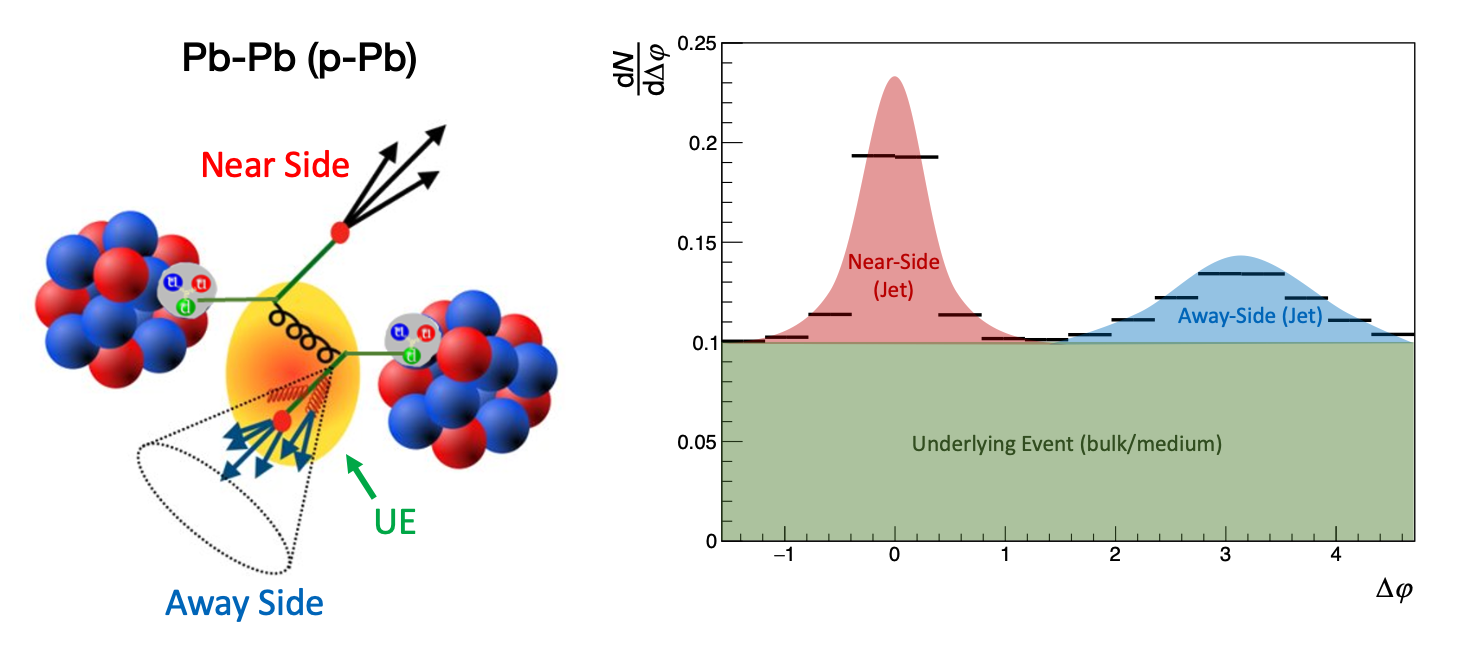
\includegraphics[width=\textwidth]{figures/mnm/dphi_cartoon.png}
\caption{A cartoon of a Pb--Pb (p--Pb) collision that produces particles in the near- and away-side jets, along with the UE. The the corresponding regions in the $\Delta\varphi$ distribution are highlighted on the right.}
\label{fig:dphi_cartoon_ref}
\end{figure}

The yields and widths presented in this section are extracted from these correlation distributions, and studied as a function of multiplicity and \lmb momentum. The same procedure is performed for charged hadrons (h-h), and the results are compared.

\section{Per-trigger $\Delta\varphi$ distributions}

The per-trigger h-h and h-\lmb $\Delta\varphi$ distributions for all multiplicity and associated \pt bins can be seen in Figure~\ref{fig:h_lambda_1d_final} (h-\lmb) and Figure~\ref{fig:h_h_1d_final} (h-h). Summarizing plots that contain both the h-\lmb and h-h distributions together for each multiplicity class for the lower ($1.5 <$ \pt $< 2.5$ \GeVc) and higher ($2.5 < $ \pt $< 4.0$ \GeVc) associated \pt bins can be seen in Figures \ref{fig:dphi_final_lowpt} and \ref{fig:dphi_final_highpt}, respectively. In the summarizing plots, the entire range along the y-axis is shown to emphasize the relative contribution to each distribution from the UE. 

In the lower associated momentum range, the UE baseline for both the h-\lmb and h-h distributions is found to increase by around a factor of three from the lowest to highest multiplicity class (0.05 to 0.17 in the h-\lmb case, 0.35 to 1 in the dihadron case). The higher associated momentum range exhibits a similar increase in the UE baseline with increasing multiplicity, but the h-\lmb baseline increases by a factor of four instead of three. The UE baseline is also found to be higher in the lower associated \pt range than in the higher range by around a factor of three in the h-\lmb case and four in the h-h case for each multiplicity class. These observations suggest that associated production in the UE region truly is ``softer'' than production in the near- and away-side regions, supporting the idea that the production in the UE is heavily linked to the QGP.

\begin{figure}[ht]
	\centering
	\begin{minipage}{0.48\textwidth}
		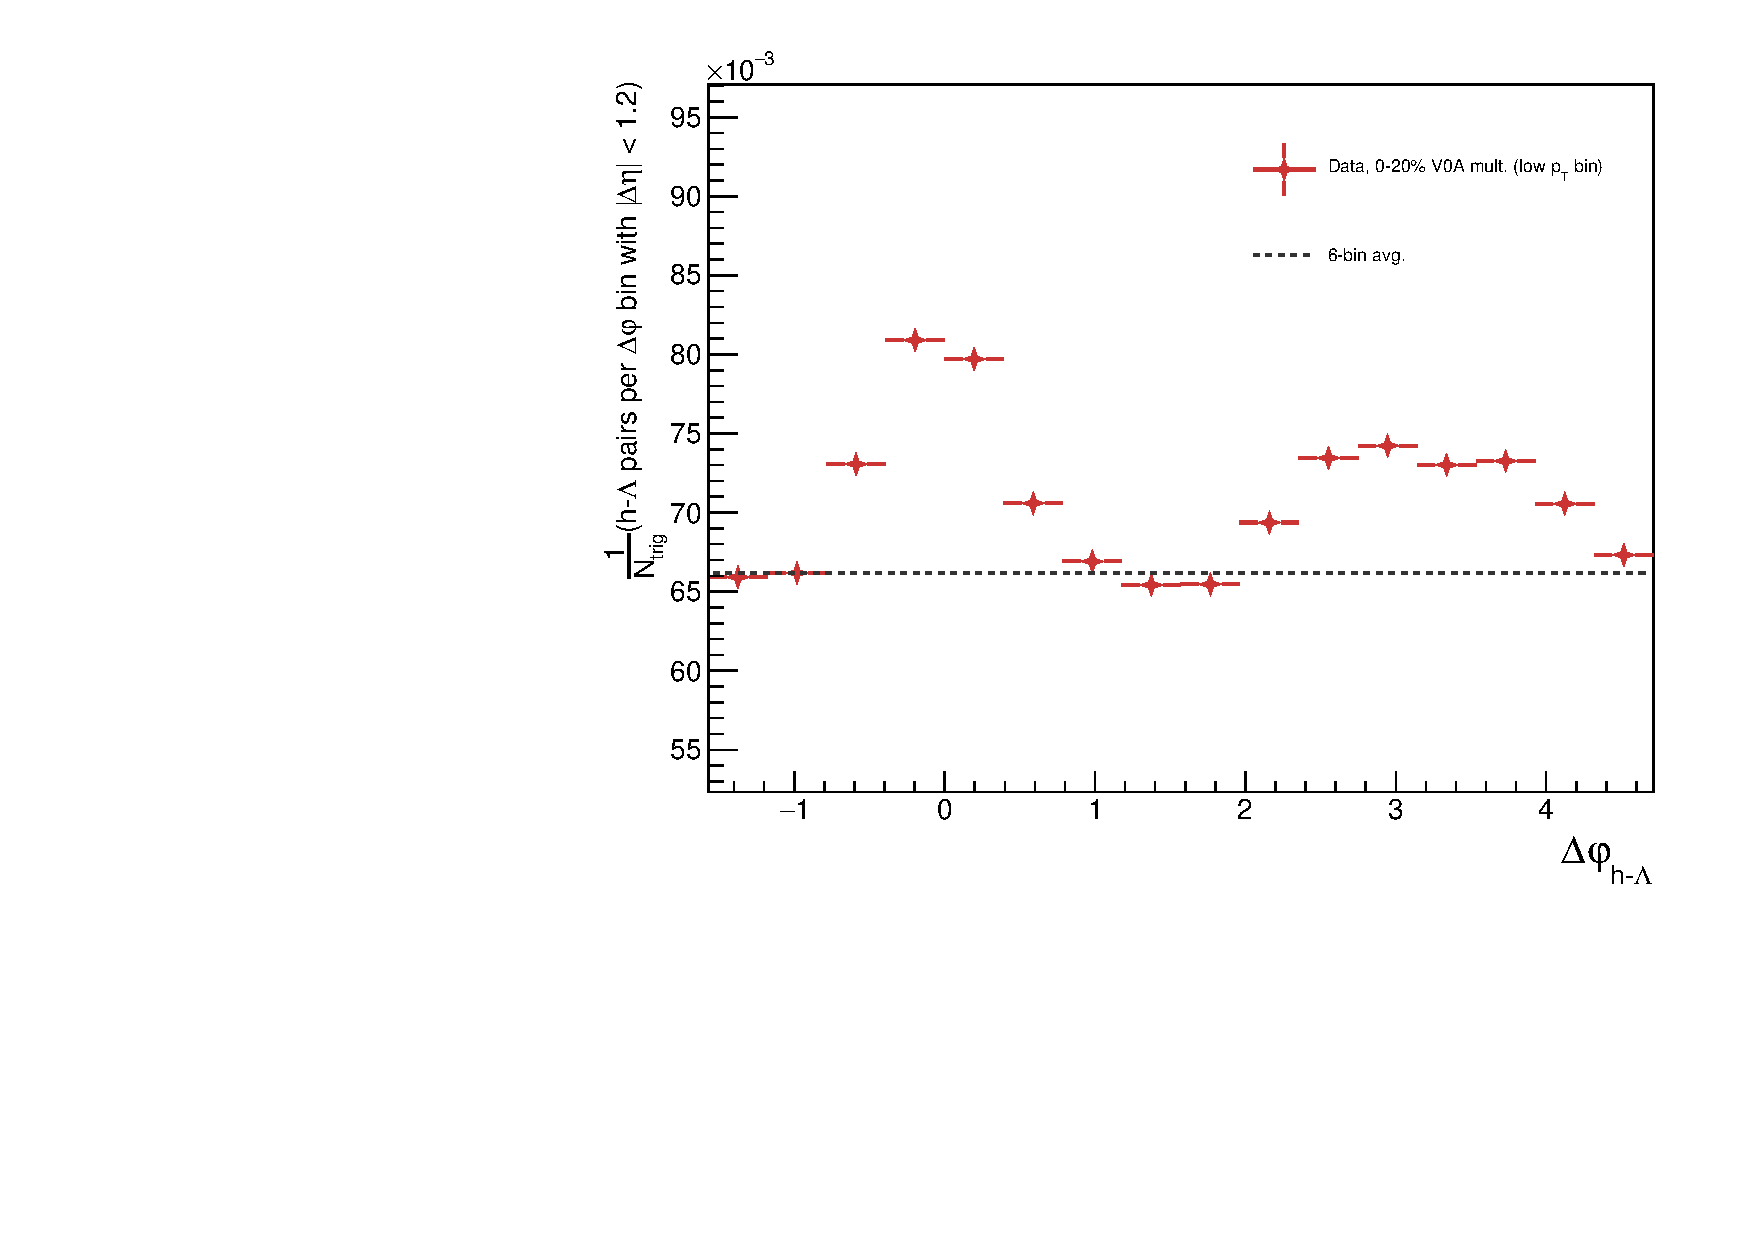
\includegraphics[width=\textwidth]{figures/analysis/h_lambda_dphi_avg6_0_20_lowpt.pdf}
	\end{minipage}
	\begin{minipage}{0.48\textwidth}
		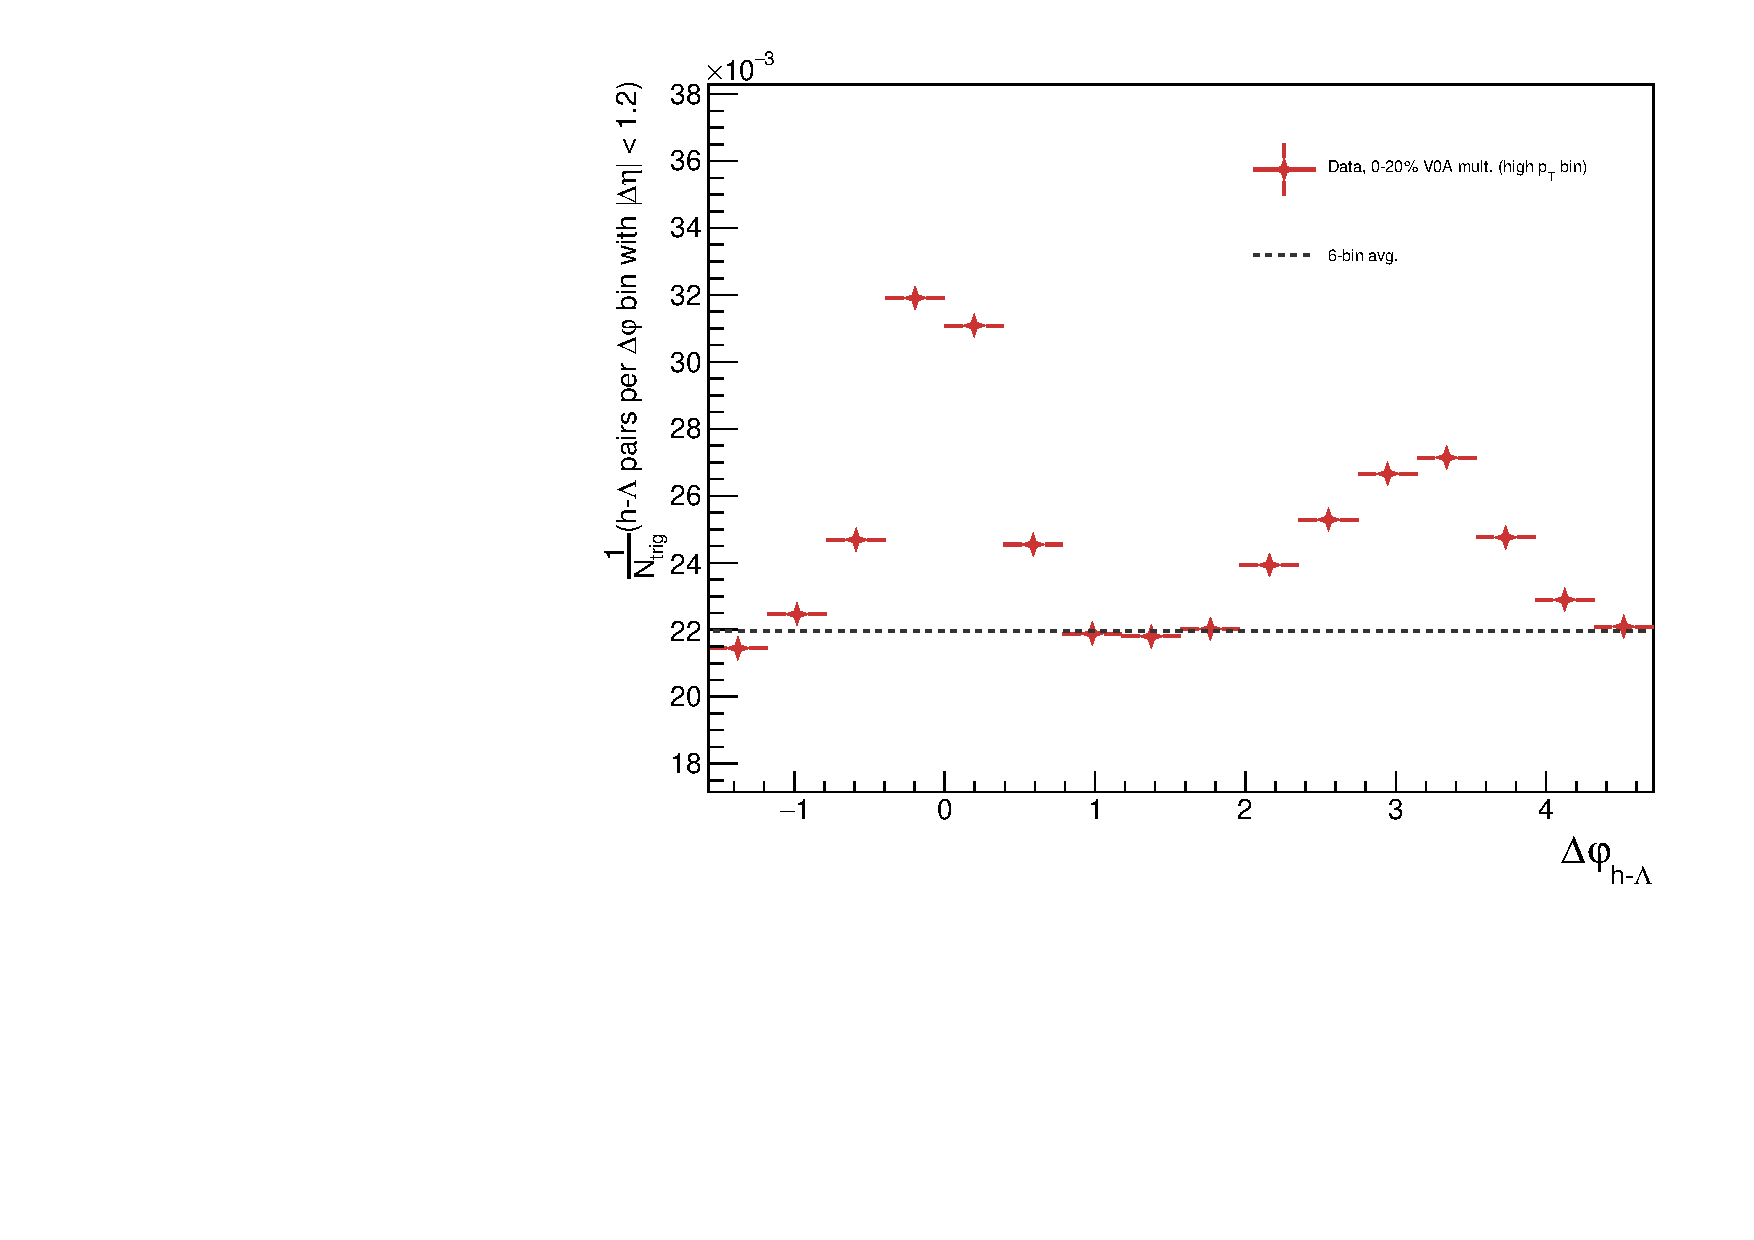
\includegraphics[width=\textwidth]{figures/analysis/h_lambda_dphi_avg6_0_20_highpt.pdf}
	\end{minipage}
	\begin{minipage}{0.48\textwidth}
		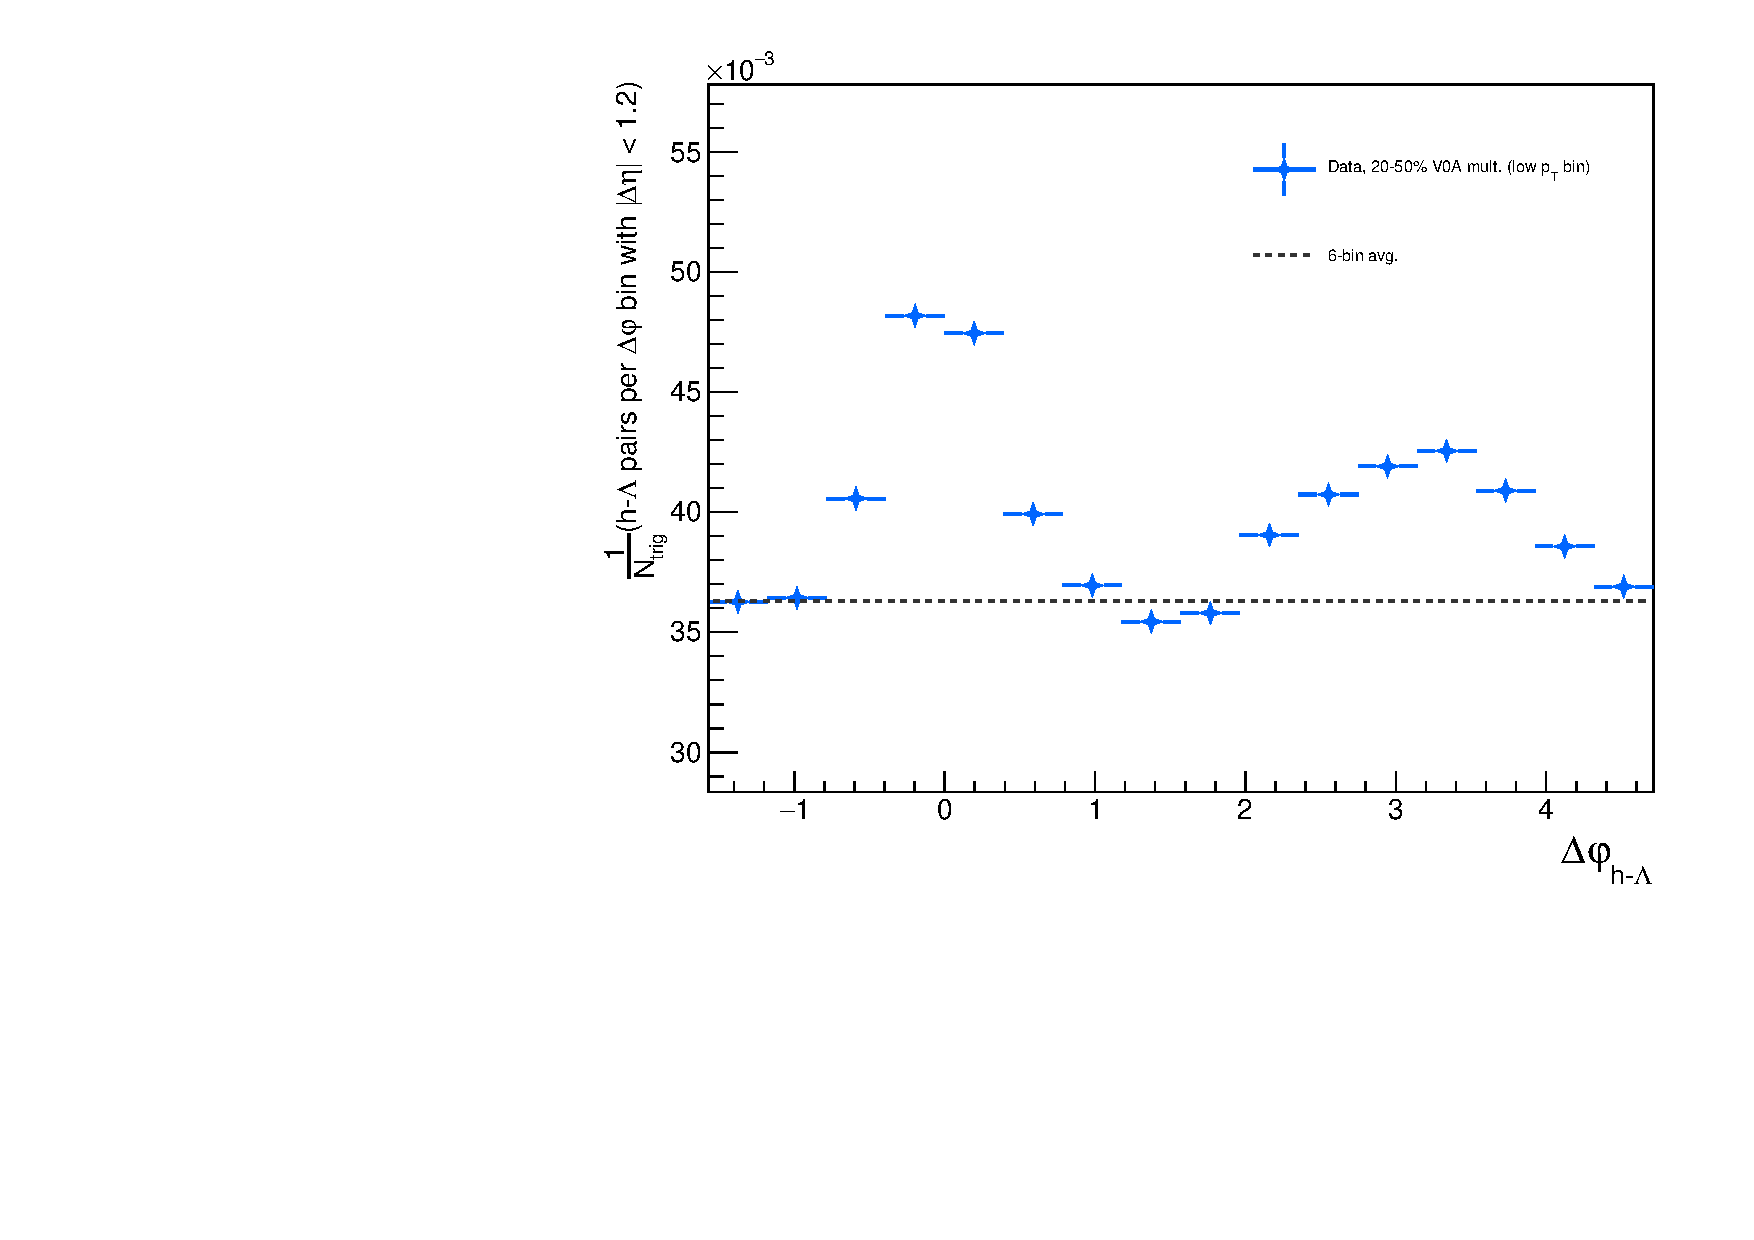
\includegraphics[width=\textwidth]{figures/analysis/h_lambda_dphi_avg6_20_50_lowpt.pdf}
	\end{minipage}
	\begin{minipage}{0.48\textwidth}
		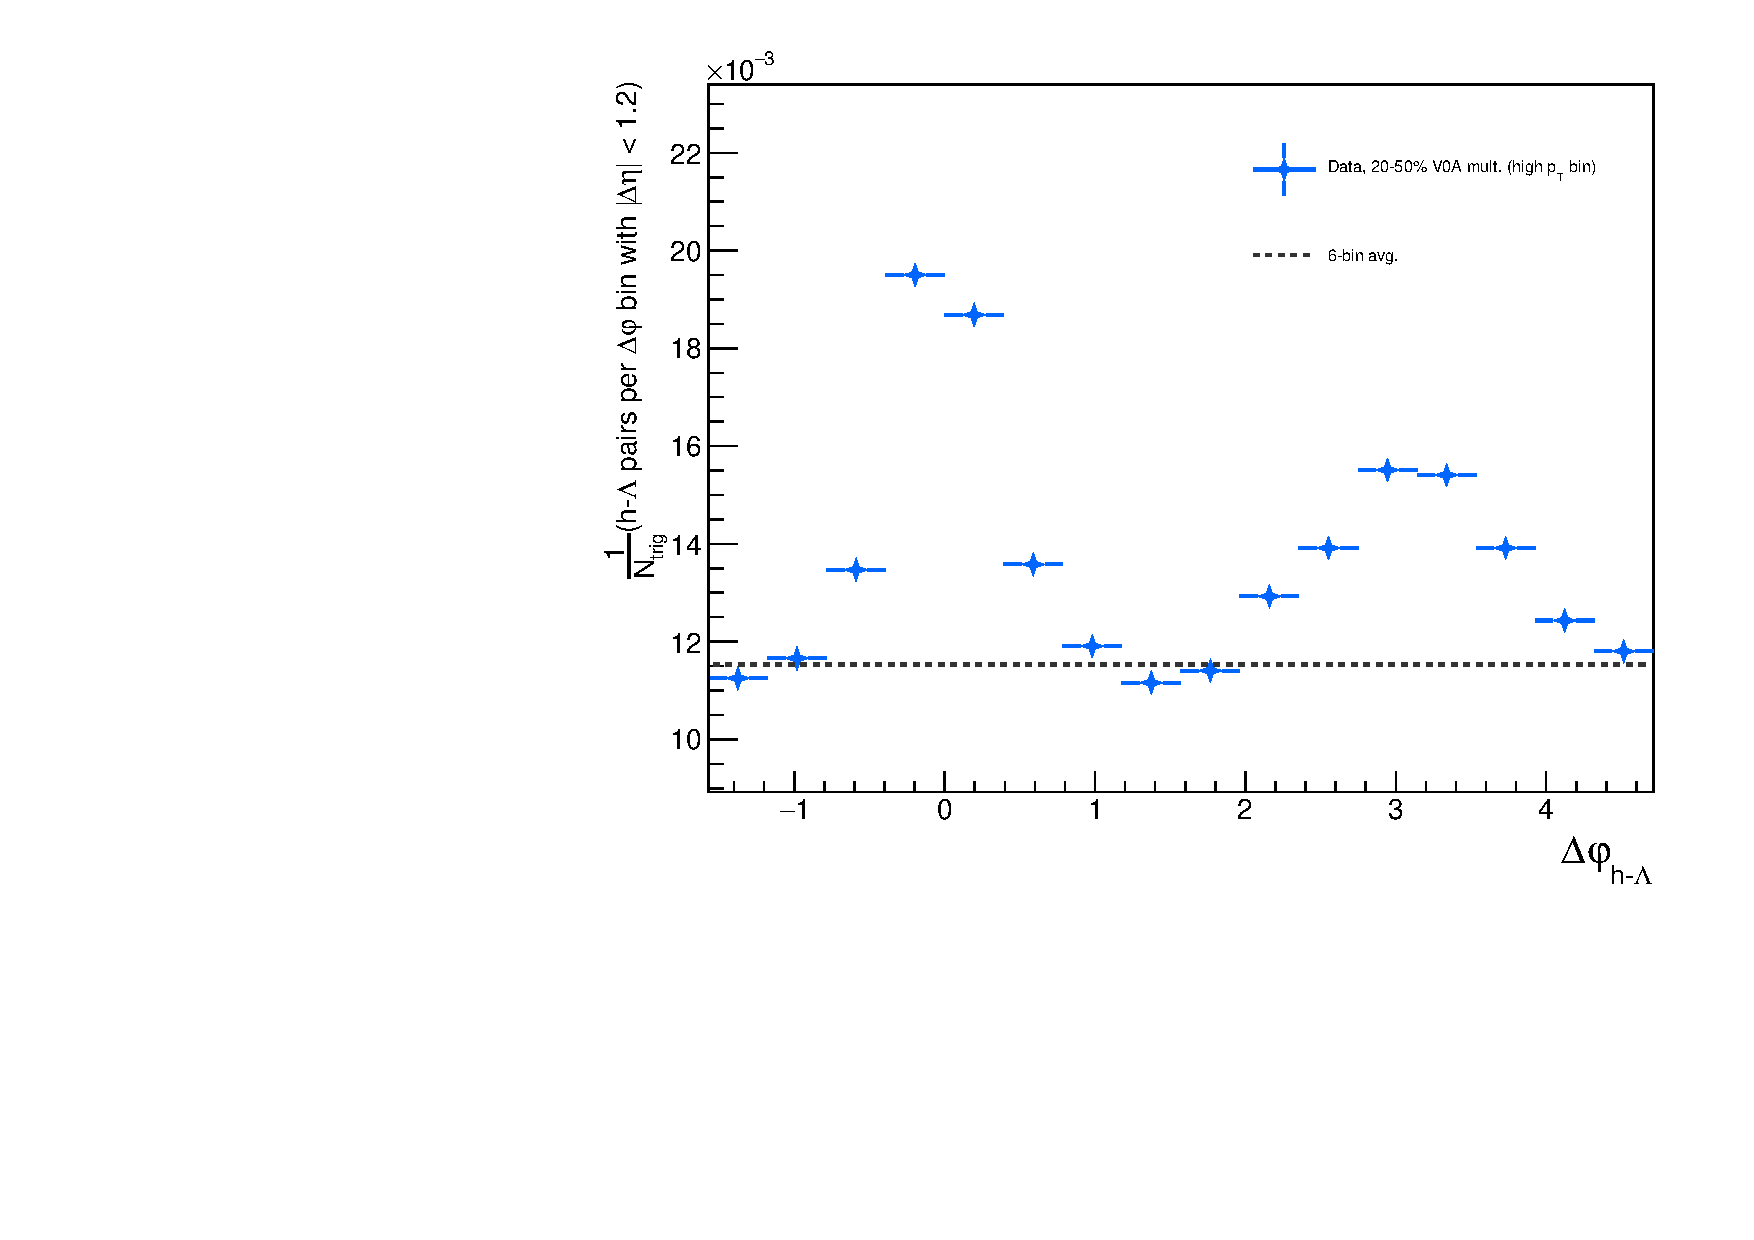
\includegraphics[width=\textwidth]{figures/analysis/h_lambda_dphi_avg6_20_50_highpt.pdf}
	\end{minipage}
	\begin{minipage}{0.48\textwidth}
		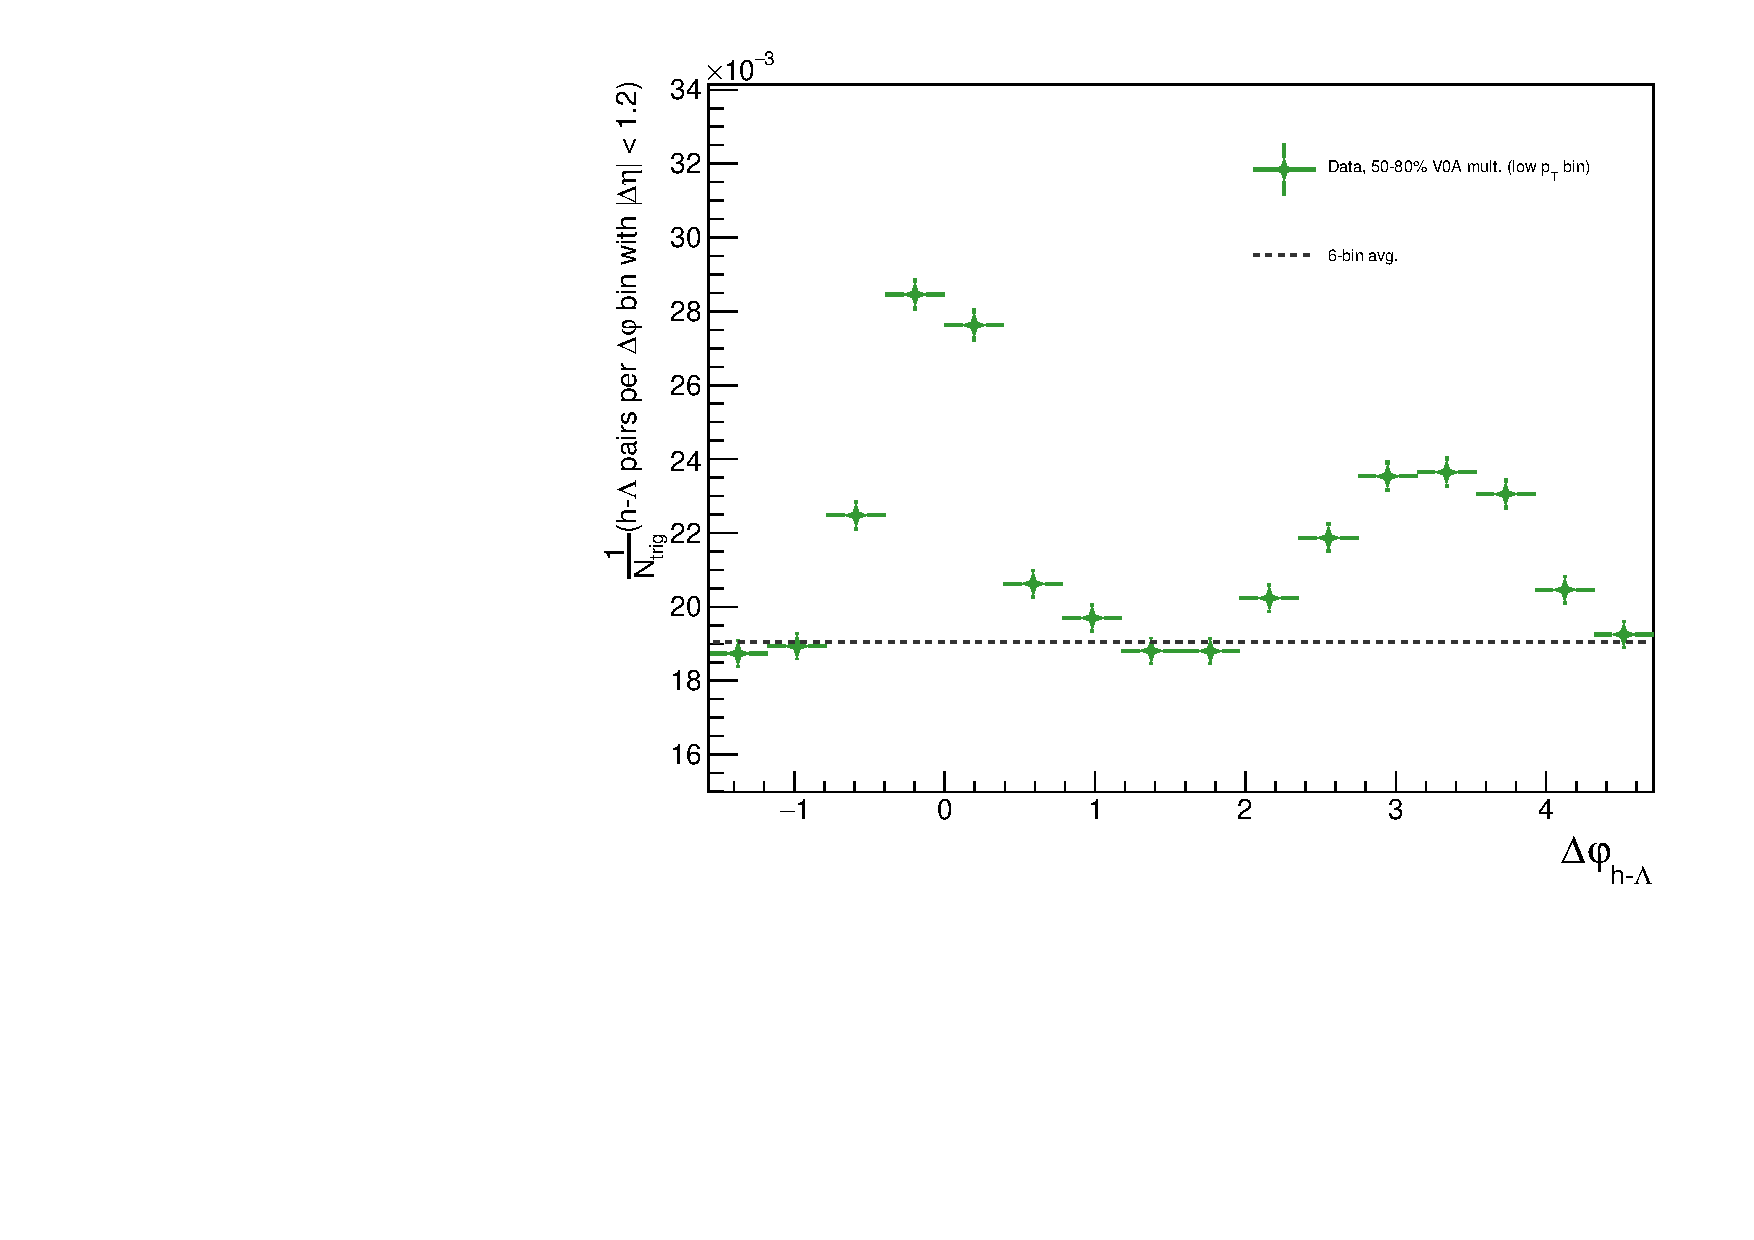
\includegraphics[width=\textwidth]{figures/analysis/h_lambda_dphi_avg6_50_80_lowpt.pdf}
	\end{minipage}
	\begin{minipage}{0.48\textwidth}
		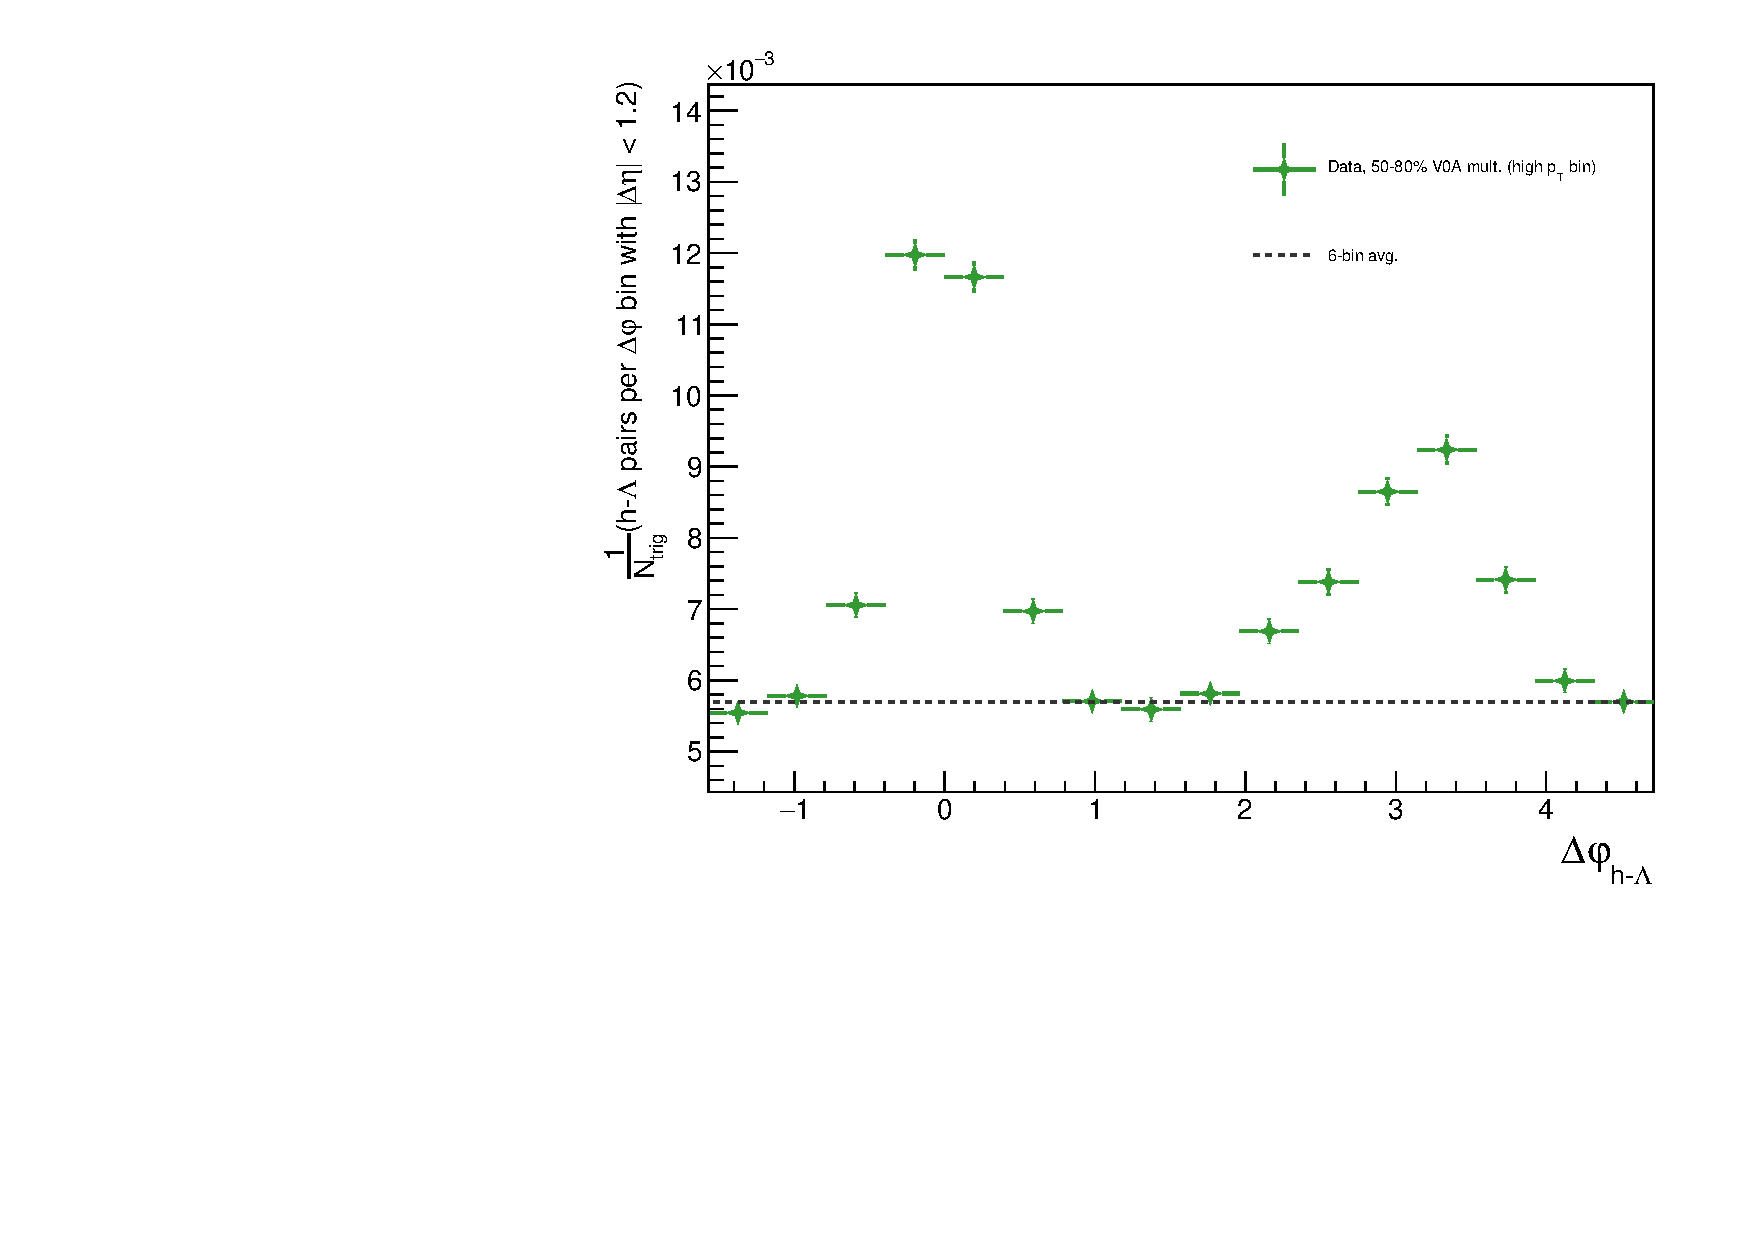
\includegraphics[width=\textwidth]{figures/analysis/h_lambda_dphi_avg6_50_80_highpt.pdf}
	\end{minipage}
	\caption{The final per-trigger h-$\Lambda$ $\Delta\varphi$ distributions for the 0-20\% (top), 20-50\% (middle), and 50-80\% (bottom) multiplicity bins for $1.5 < p_{\text{T}} < 2.5$ GeV/$c$ (left) and $2.5 < p_{\text{T}} < 4.0$ GeV/$c$ (right).}
	\label{fig:h_lambda_1d_final}
\end{figure}

\begin{figure}[ht]
	\centering
	\begin{minipage}{0.48\textwidth}
		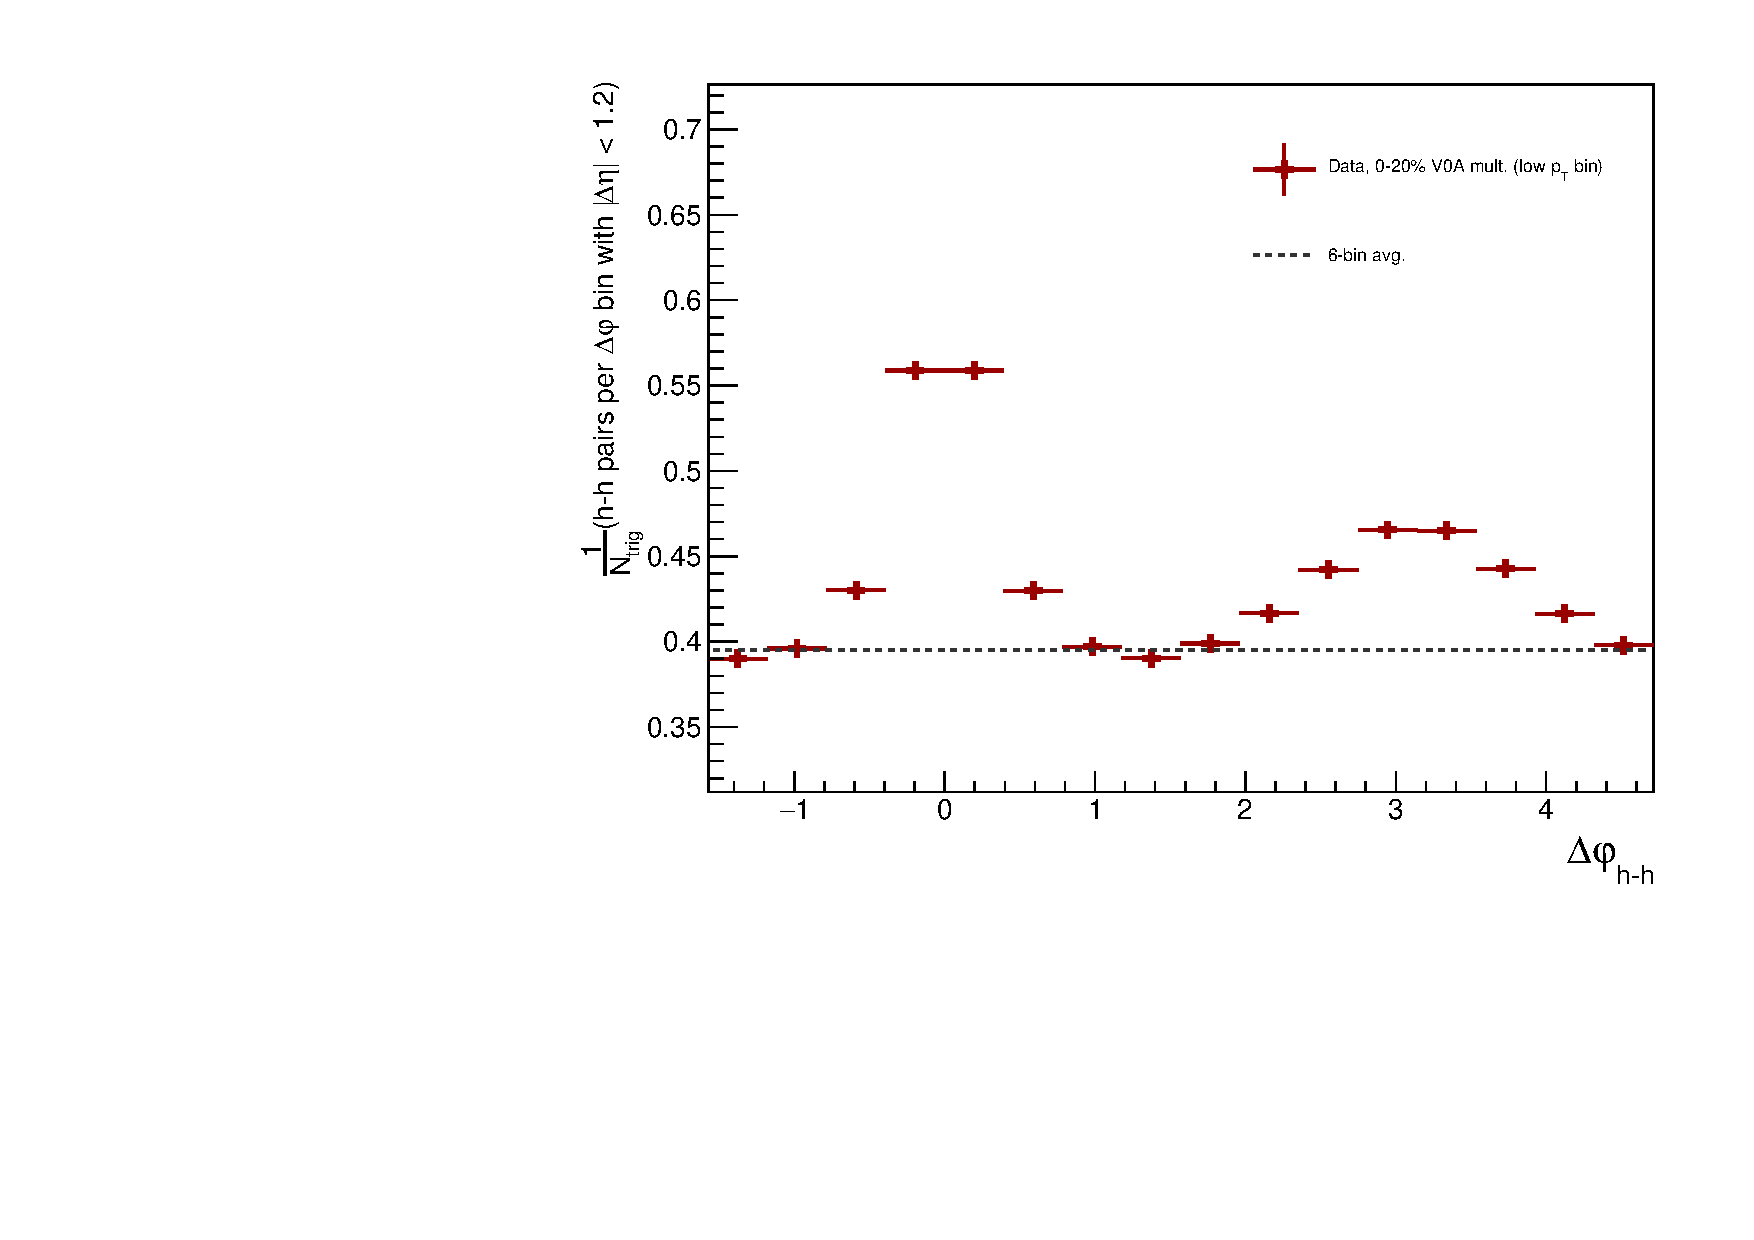
\includegraphics[width=\textwidth]{figures/analysis/h_h_dphi_avg6_0_20_lowpt.pdf}
	\end{minipage}
	\begin{minipage}{0.48\textwidth}
		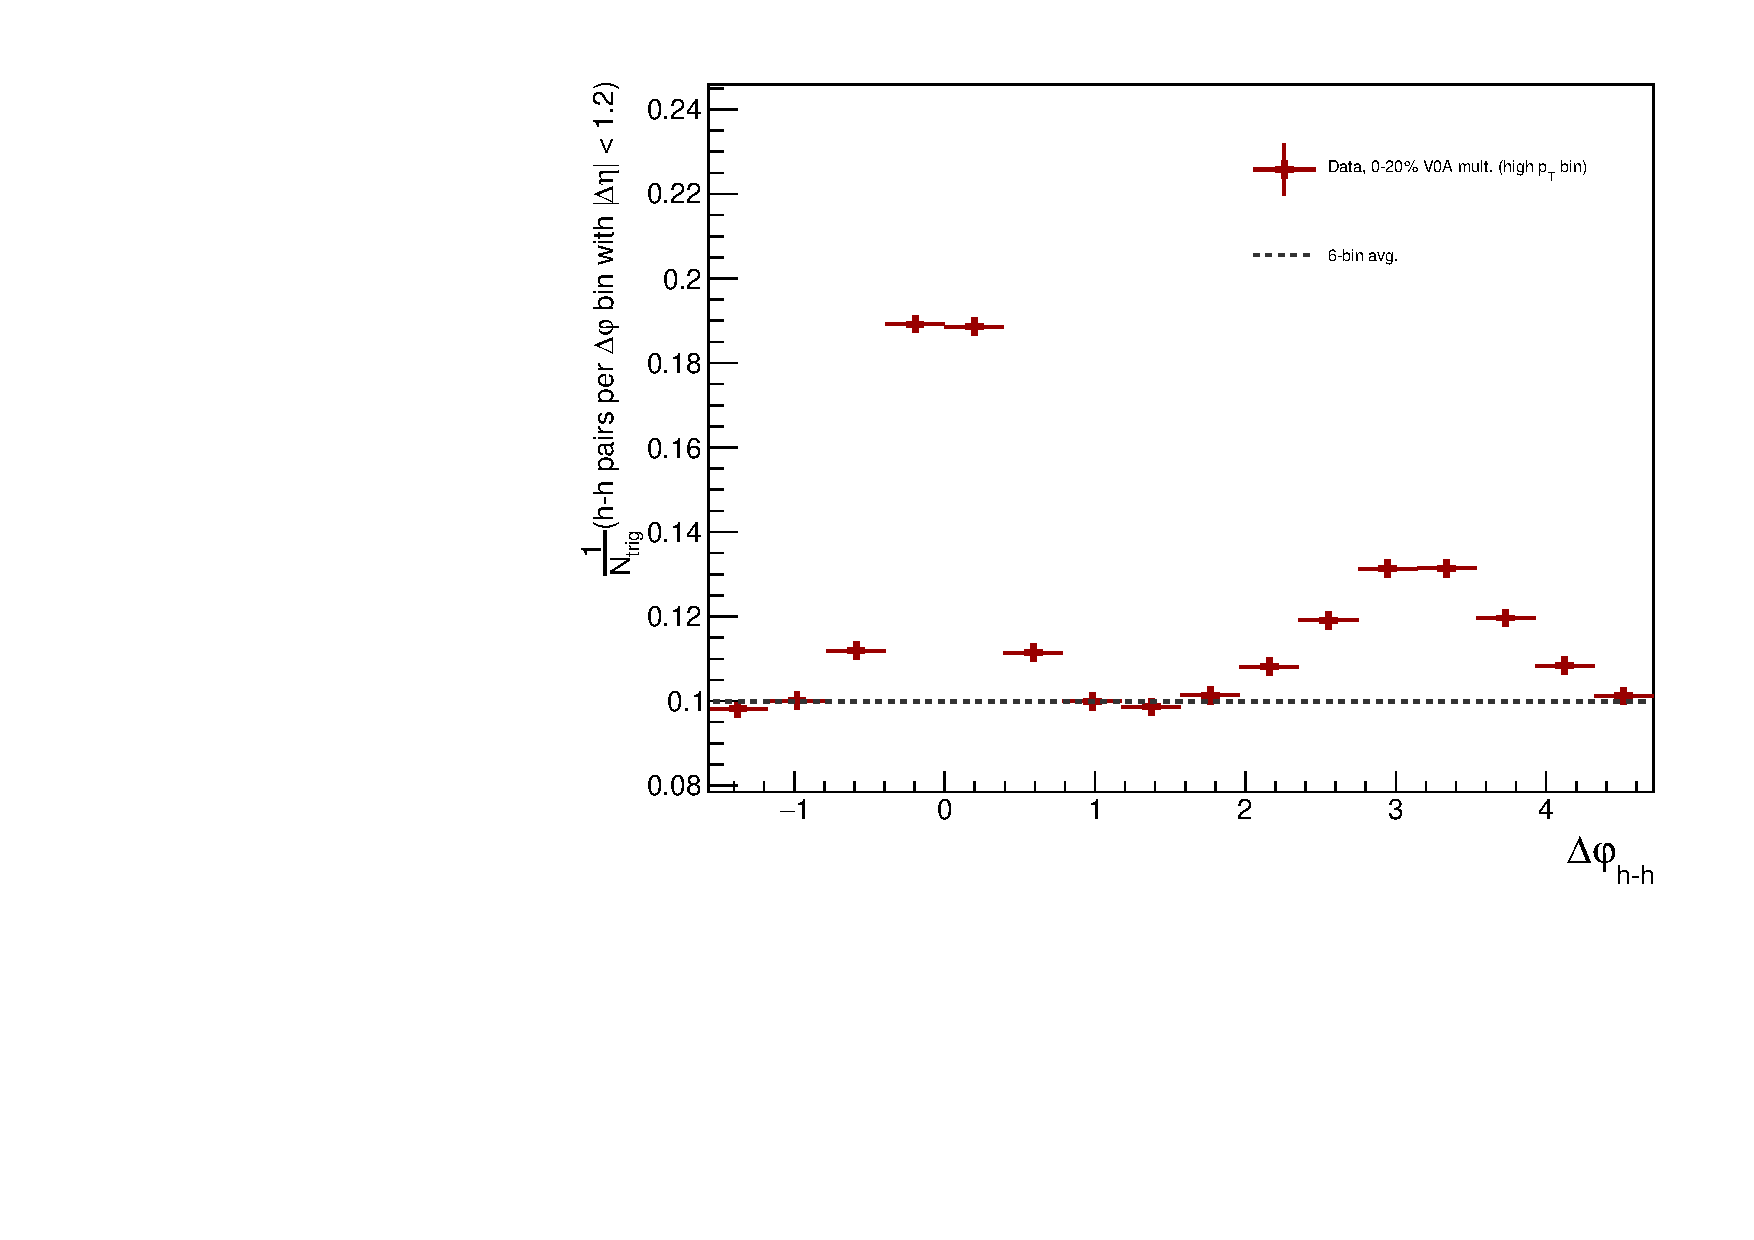
\includegraphics[width=\textwidth]{figures/analysis/h_h_dphi_avg6_0_20_highpt.pdf}
	\end{minipage}
	\begin{minipage}{0.48\textwidth}
		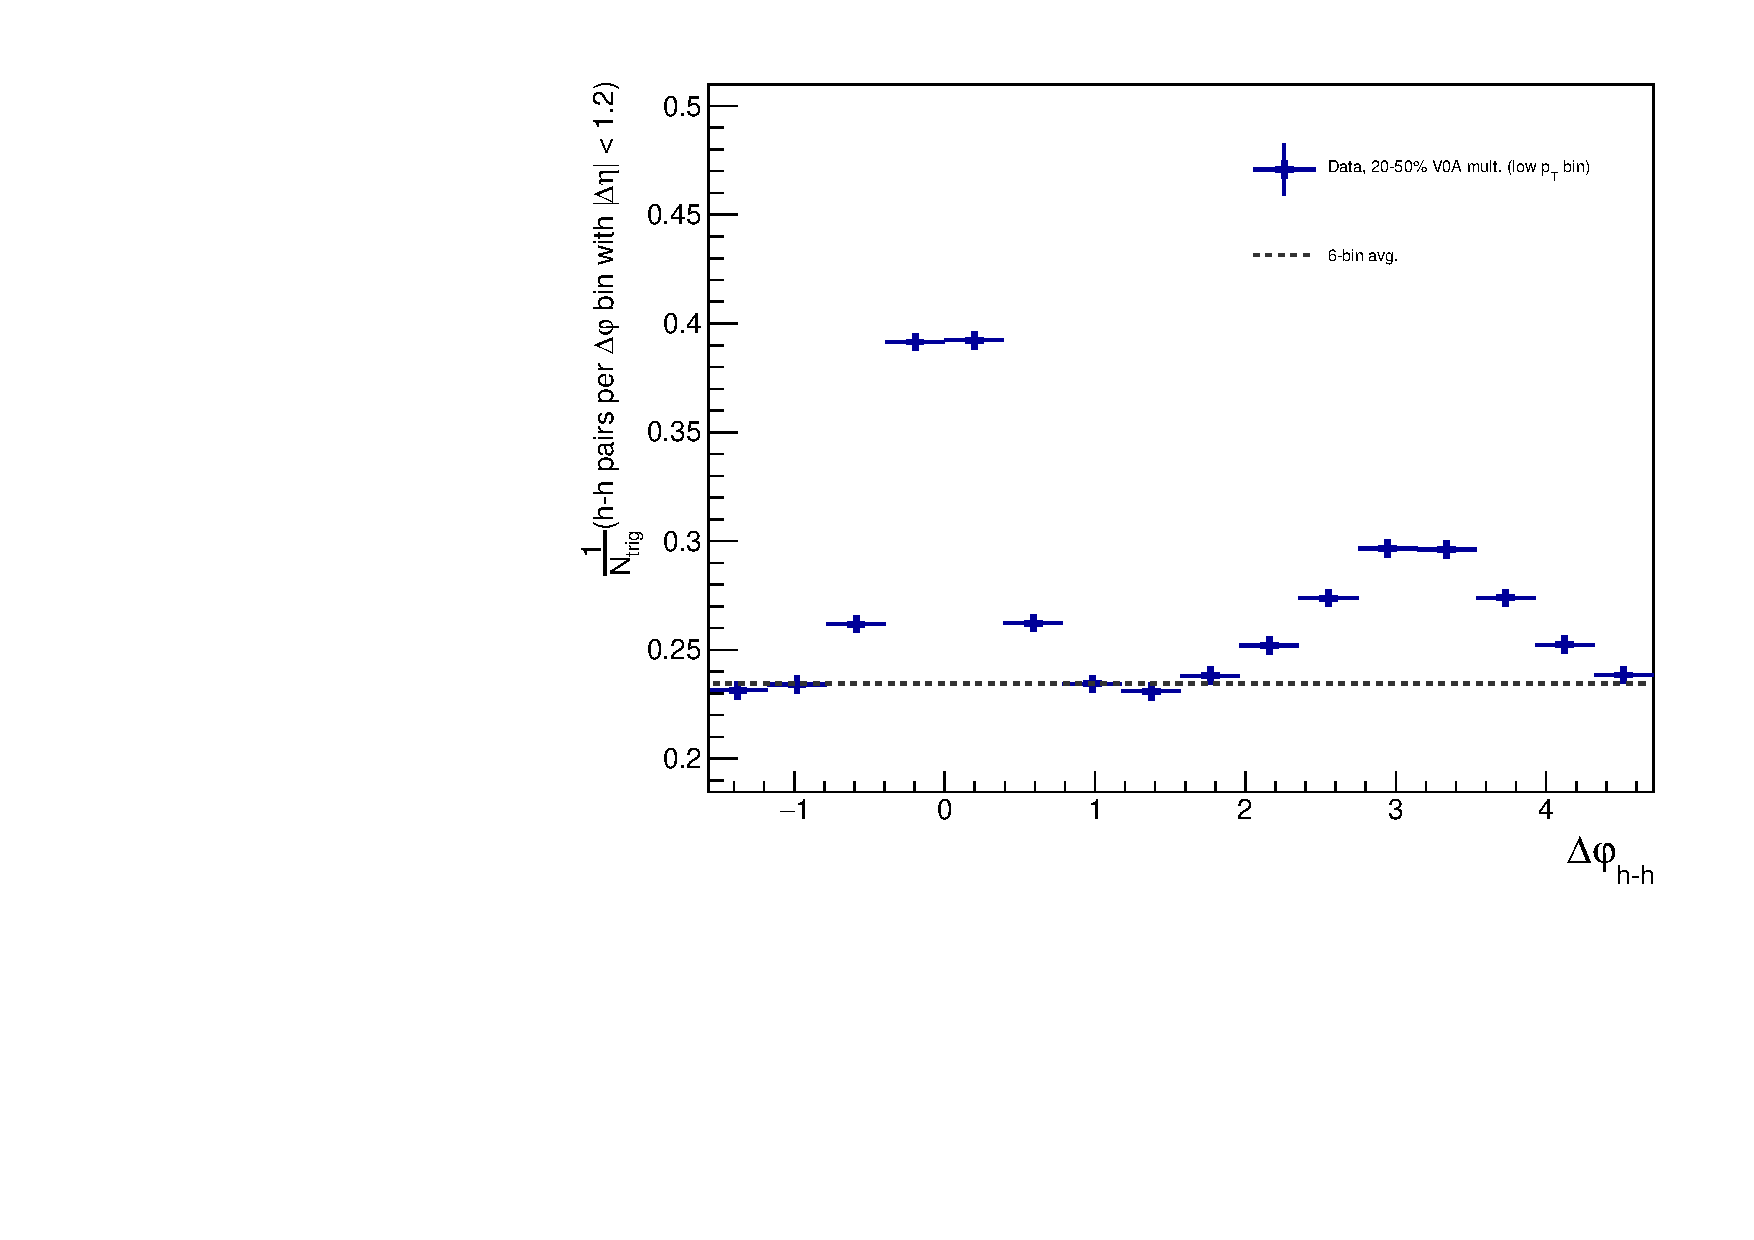
\includegraphics[width=\textwidth]{figures/analysis/h_h_dphi_avg6_20_50_lowpt.pdf}
	\end{minipage}
	\begin{minipage}{0.48\textwidth}
		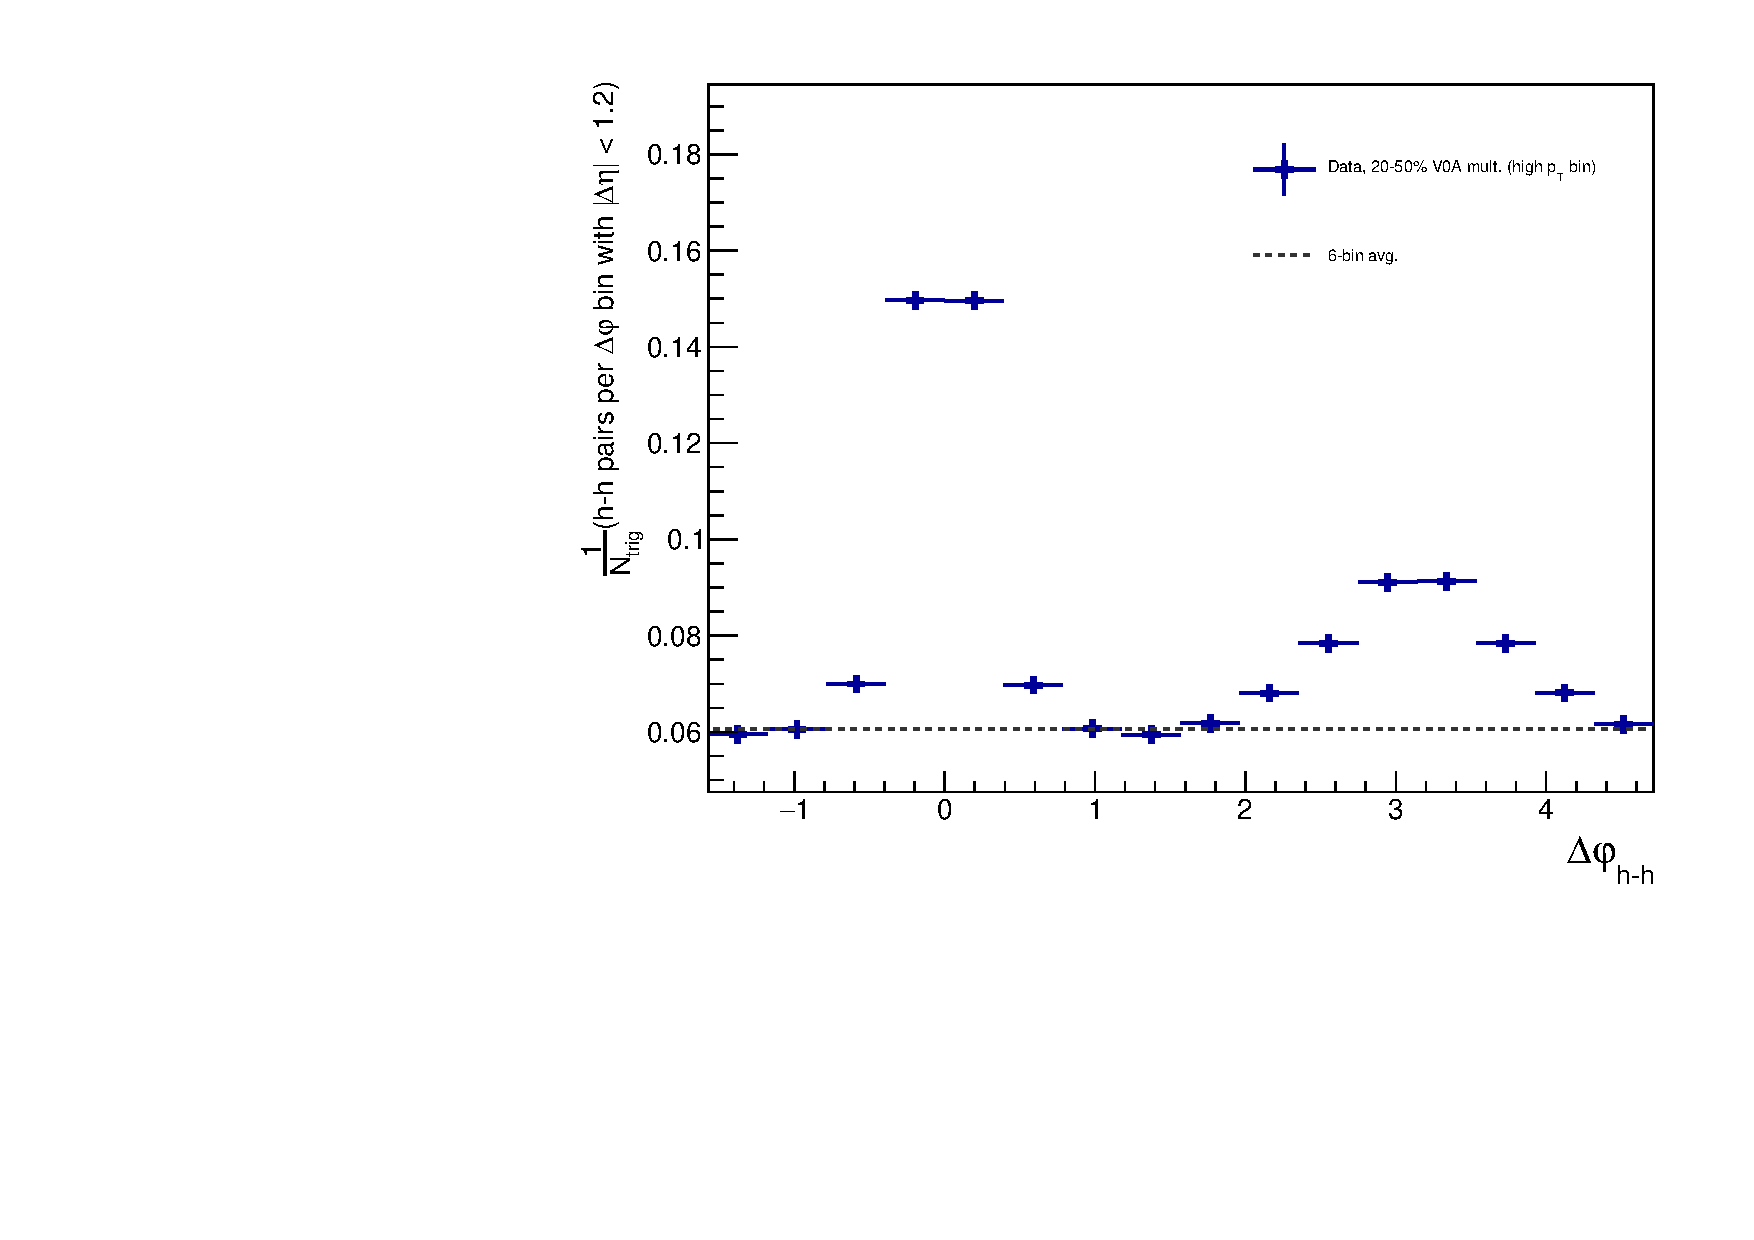
\includegraphics[width=\textwidth]{figures/analysis/h_h_dphi_avg6_20_50_highpt.pdf}
	\end{minipage}
	\begin{minipage}{0.48\textwidth}
		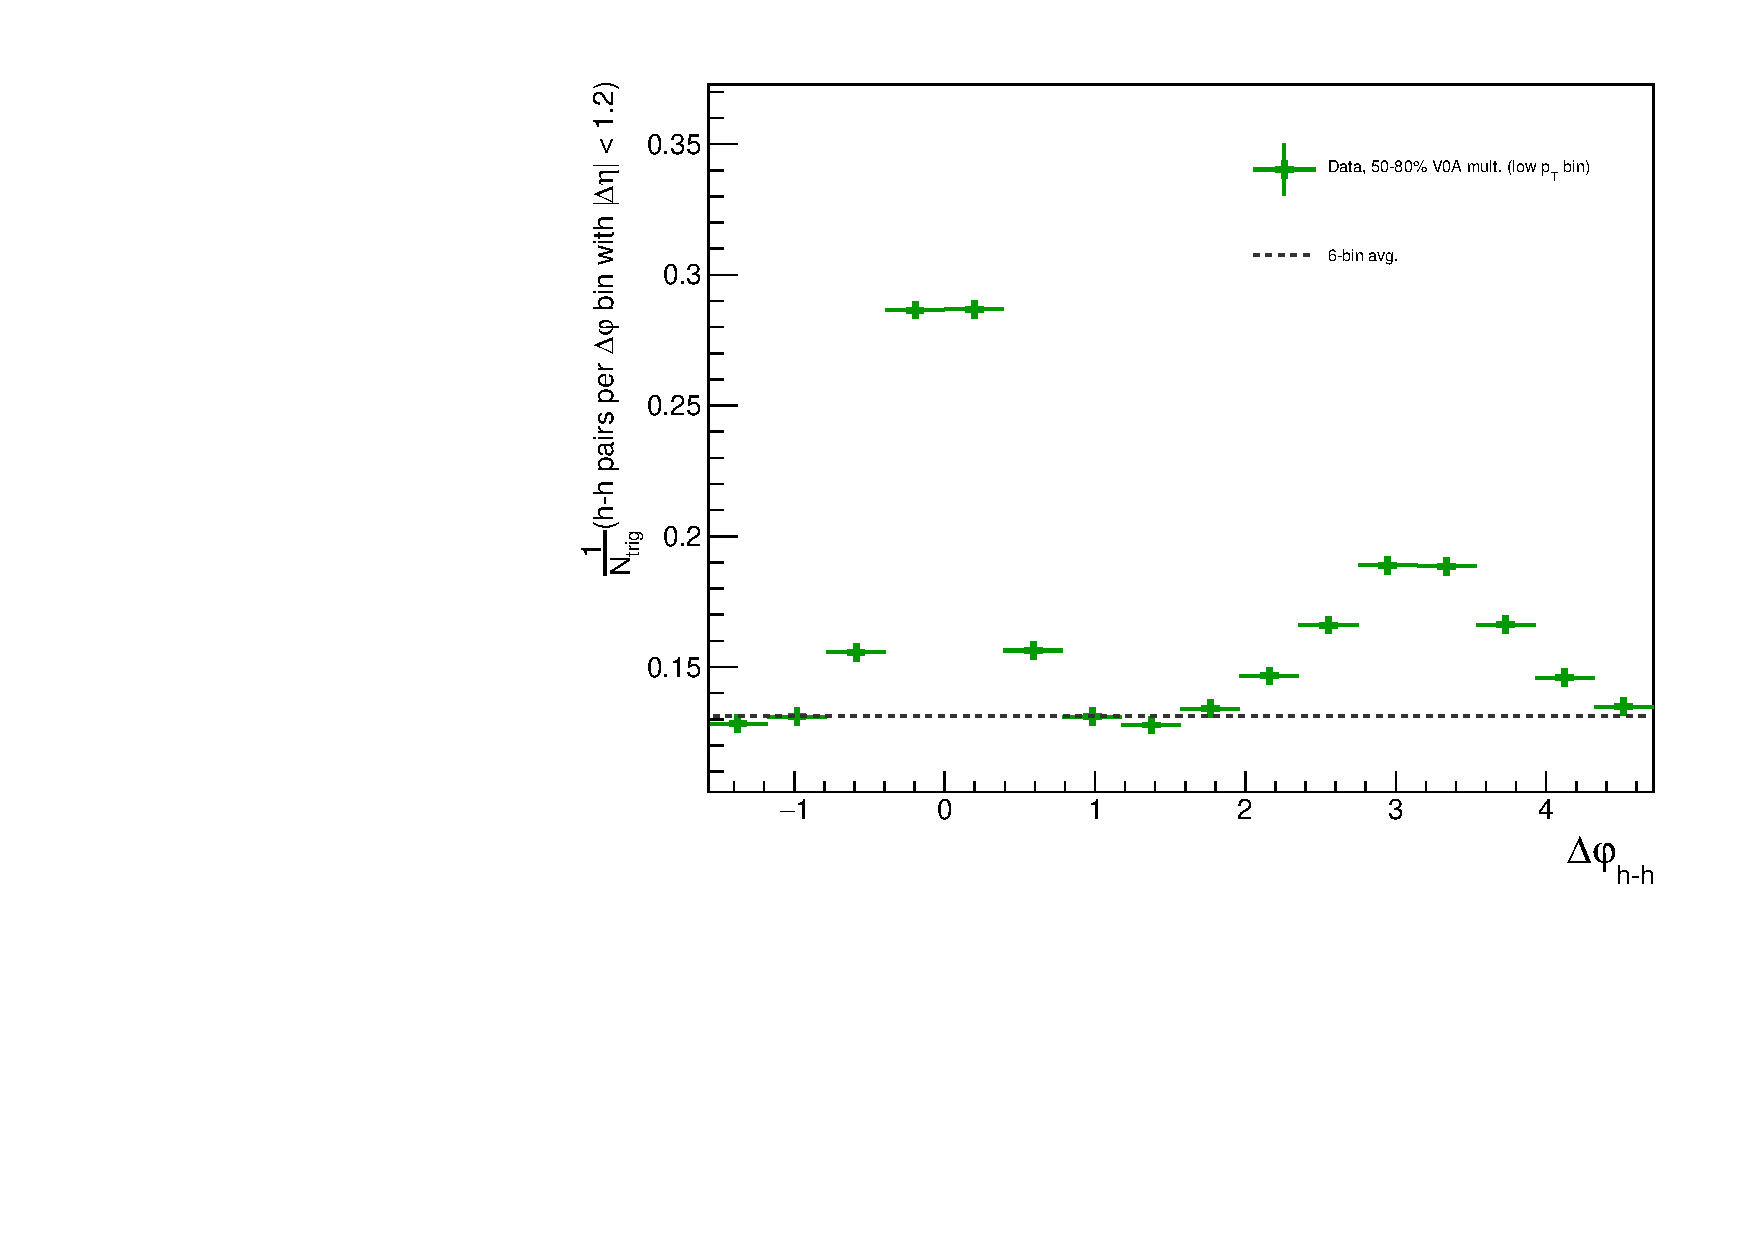
\includegraphics[width=\textwidth]{figures/analysis/h_h_dphi_avg6_50_80_lowpt.pdf}
	\end{minipage}
	\begin{minipage}{0.48\textwidth}
		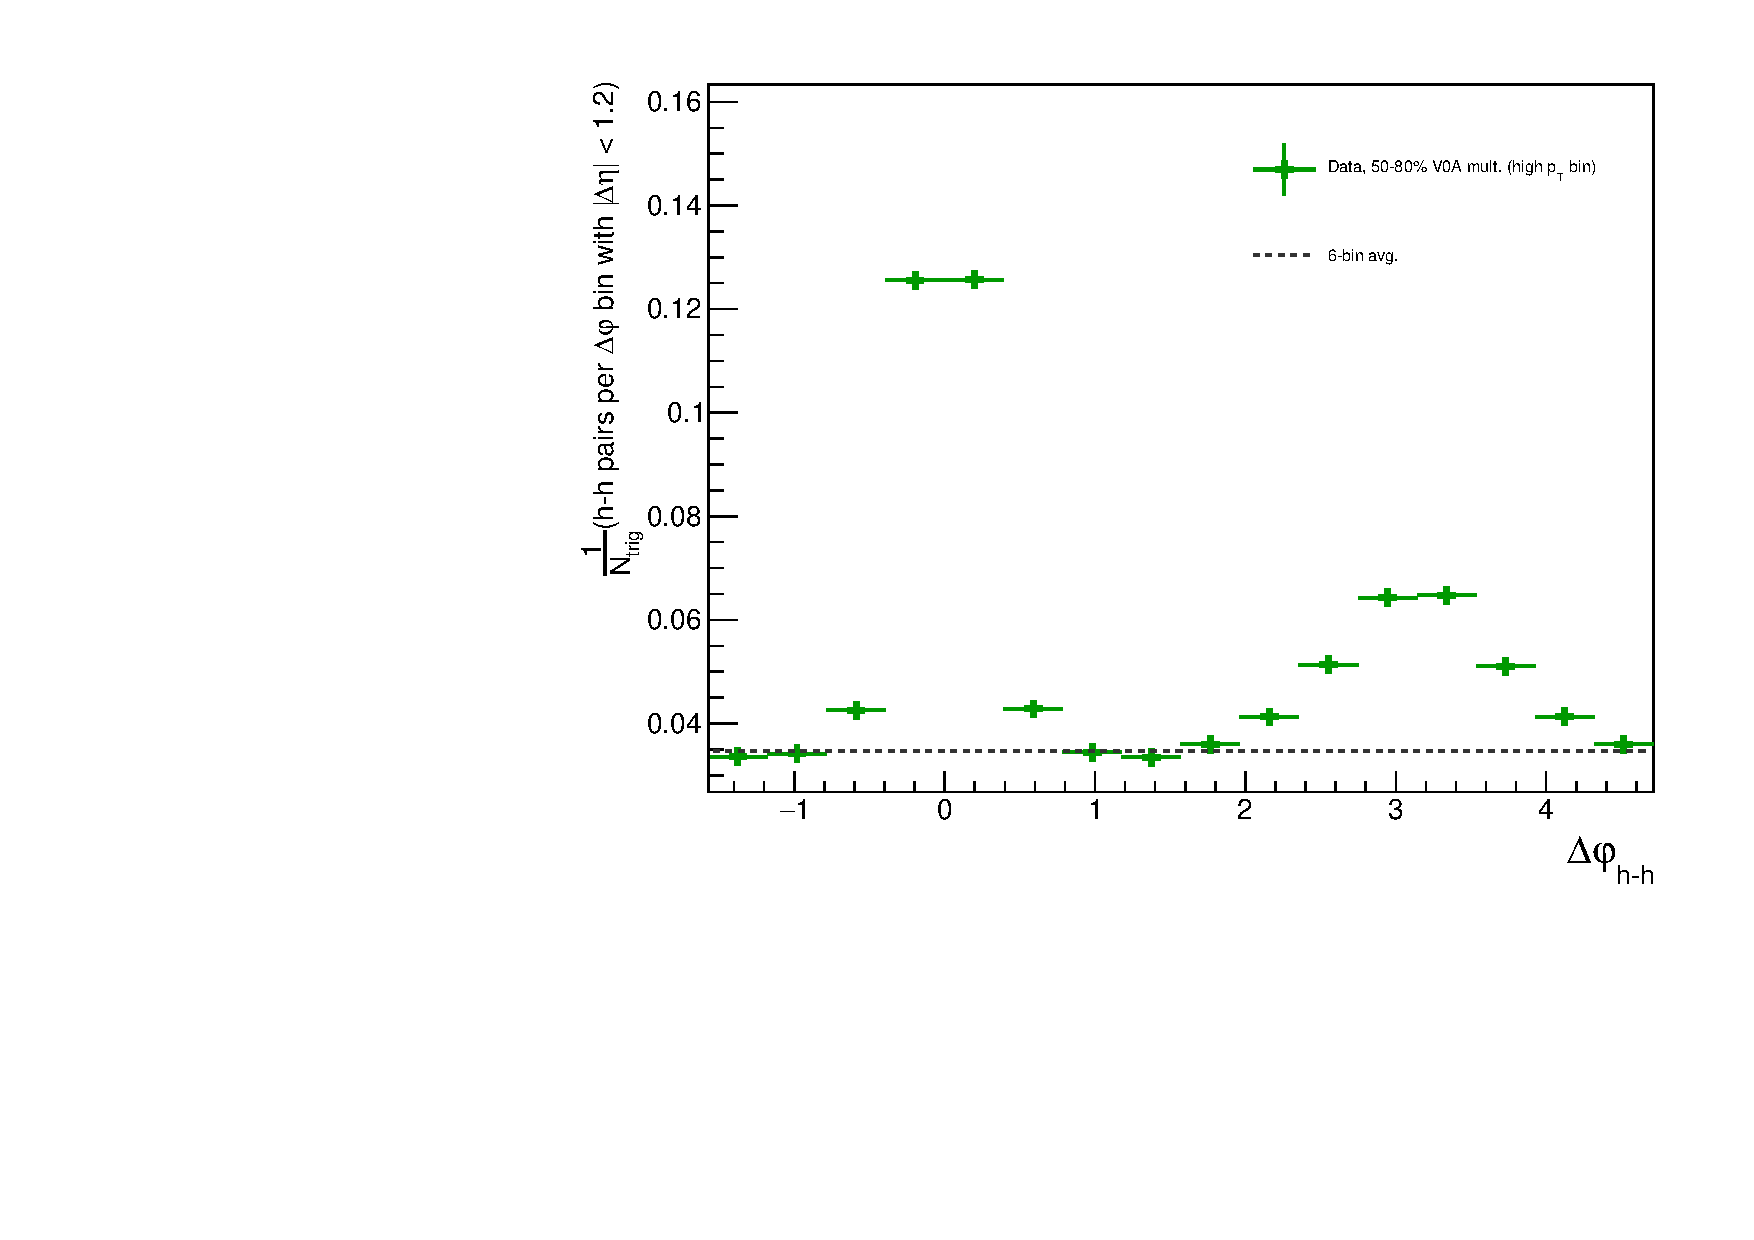
\includegraphics[width=\textwidth]{figures/analysis/h_h_dphi_avg6_50_80_highpt.pdf}
	\end{minipage}
	\caption{The final per-trigger h-h $\Delta\varphi$ distributions for the 0-20\% (top), 20-50\% (middle), and 50-80\% (bottom) multiplicity bins for $1.5 < p_{\text{T}} < 2.5$ GeV/$c$ (left) and $2.5 < p_{\text{T}} < 4.0$ GeV/$c$ (right).}
	\label{fig:h_h_1d_final}
\end{figure}

\begin{figure}[h!]
\centering
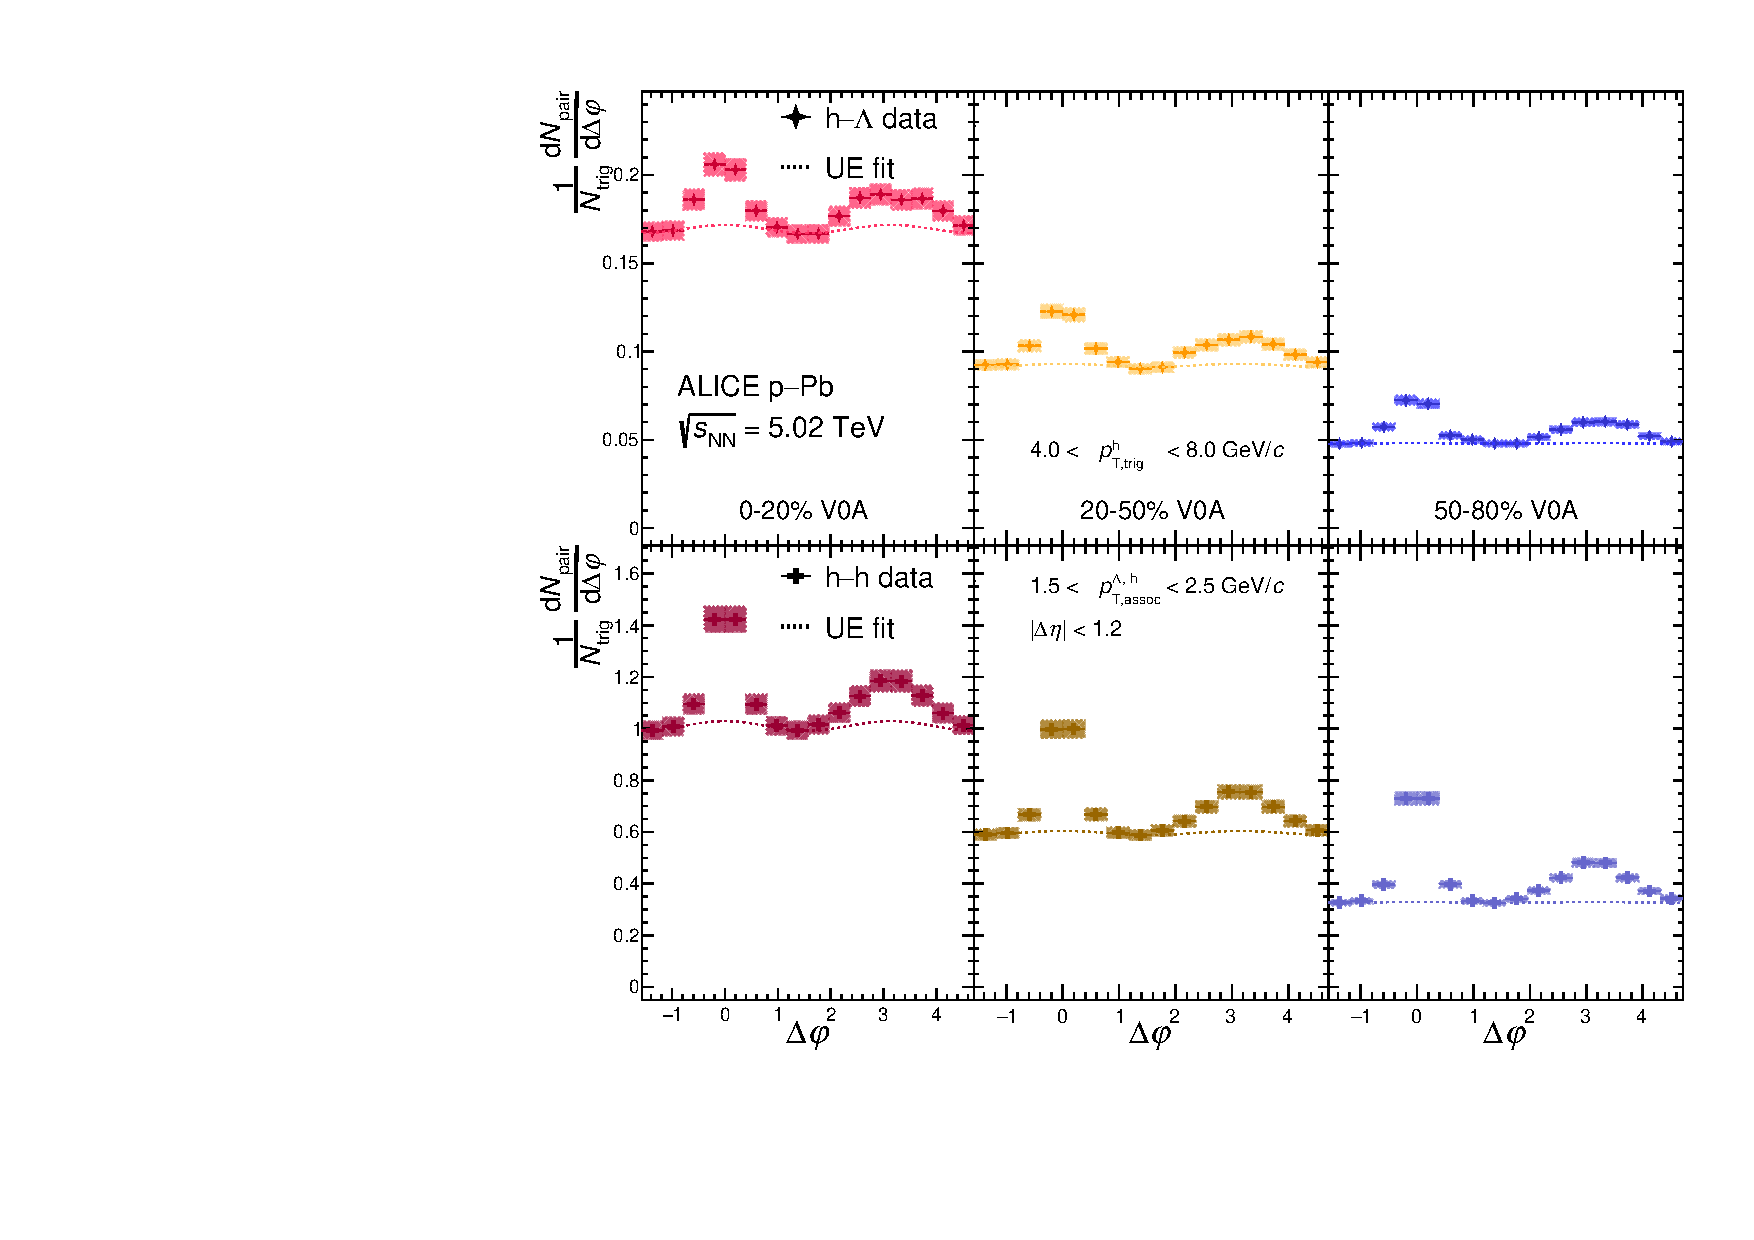
\includegraphics[width=0.83\textwidth]{figures/results/dphi_final_lowpt.pdf}
\caption{The h-$\Lambda$ (top) and h-h (bottom) $\Delta\varphi$ distributions for each multiplicity class with $1.5 < p_{\text{T,assoc}} < 2.5$ \GeVc, with statistical (systematic) uncertainties shown as vertical lines (shaded boxes). The multiplicity classes are plotted from most central (left) to least central (right). The UE estimate is shown as a dashed line, and is taken as the average of the distribution in the regions $[-\frac{\pi}{2}, -\frac{\pi}{4}) \cup [\frac{\pi}{4}, \frac{5\pi}{8}) \cup [\frac{11\pi}{8}, \frac{3\pi}{2})$.}
\label{fig:dphi_final_lowpt}
\end{figure}

\begin{figure}[h!]
\centering
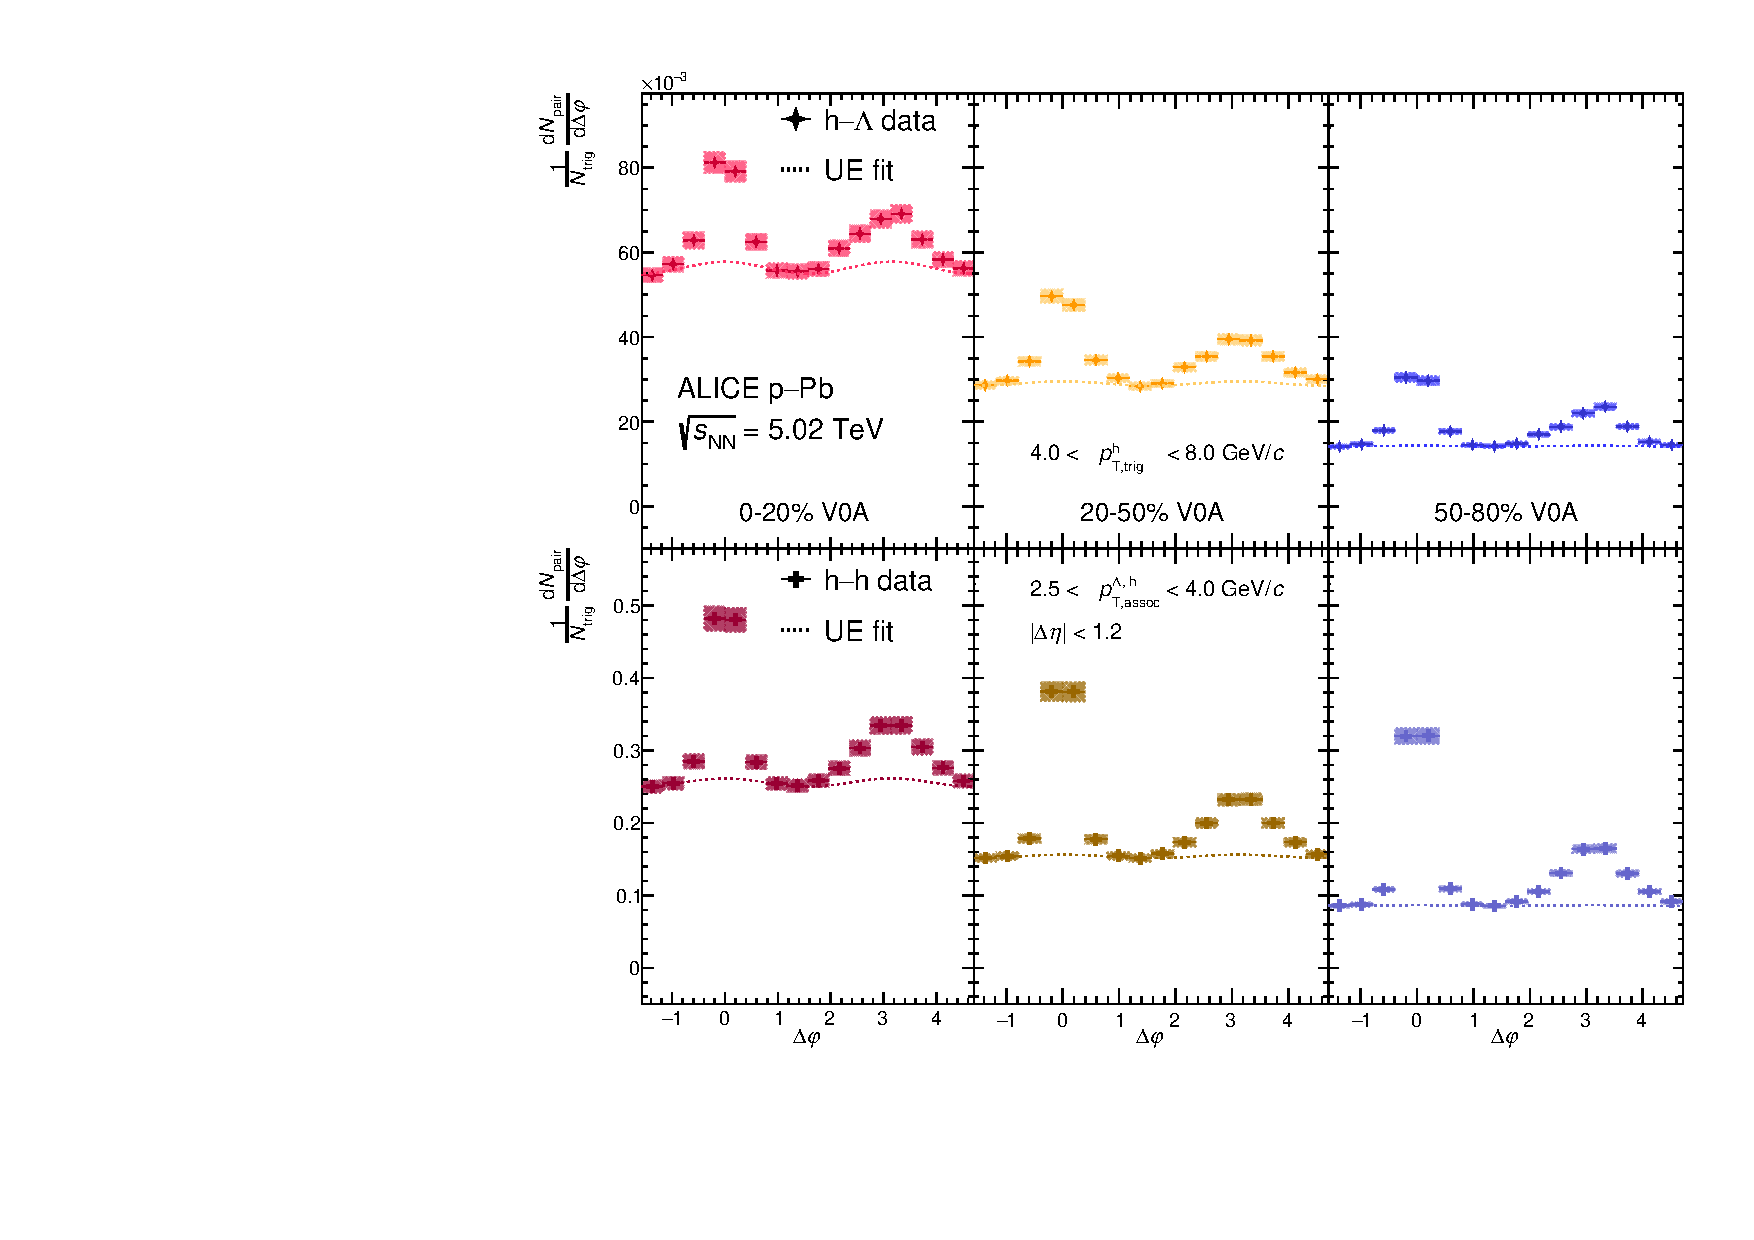
\includegraphics[width=0.83\textwidth]{figures/results/dphi_final_highpt.pdf}
\caption{The h-$\Lambda$ (top) and h-h (bottom) $\Delta\varphi$ distributions for each multiplicity class with $2.5 < p_{\text{T,assoc}} < 4.0$ \GeVc, with statistical (systematic) uncertainties shown as vertical lines (shaded boxes). The multiplicity classes are plotted from most central (left) to least central (right). The UE estimate is shown as a dashed line, and is taken as the average of the distribution in the regions $[-\frac{\pi}{2}, -\frac{\pi}{4}) \cup [\frac{\pi}{4}, \frac{5\pi}{8}) \cup [\frac{11\pi}{8}, \frac{3\pi}{2})$.}
\label{fig:dphi_final_highpt}
\end{figure}

\section{Per-trigger yields and jet-like region widths}

The per-trigger yields in the near- and away-side regions of the $\Delta\varphi$ distributions ($Y_{\text{near}}$, $Y_{\text{away}}$) are shown in each associated \pt range as a function of multiplicity for both the h-$\Lambda$ and dihadron correlations in Figure \ref{fig:pairwise_yield}. Straight line fits of the data are shown as dashed lines. To improve comparibility with previous results~\cite{ALICEpPbEnhancement,ALICEppEnhancement}, the multiplicity classes have been converted to charged particle multiplicity by computing $\langle$\dndeta$\rangle$ in each multiplicity class in events with a trigger hadron for all charged hadrons with $|\eta| < 0.5$ and $p_{\text{T}} > 0.15$ \GeVc. The values of $\langle$\dndeta$\rangle$ for each multiplicity class in non-triggered and triggered events can be seen in Table~\ref{tab:dndeta}. 

\begin{table}
\centering
\caption{The values of $\langle$\dndeta$\rangle_{|\eta_{\text{lab}}| < 0.5}$ for each multiplicity class in min bias events (non-triggered) and events with a trigger hadron (triggered events).}
\begin{tabular}{l c c }
\hline
Mult. class & $\langle$\dndeta$\rangle$ (non-triggered) & $\langle$\dndeta$\rangle$ (triggered) \\
\hline
0-20\% & $35.6 \pm 0.9$ & $42.4 \pm 0.9$ \\
20-50\% & $21.5 \pm 0.5$ & $27.6 \pm 0.5$ \\
50-80\% & $12.0 \pm 0.3$ & $17.7 \pm 0.4$ \\
\hline
\end{tabular}
\label{tab:dndeta}
\end{table}



\begin{figure}[h!]
\centering
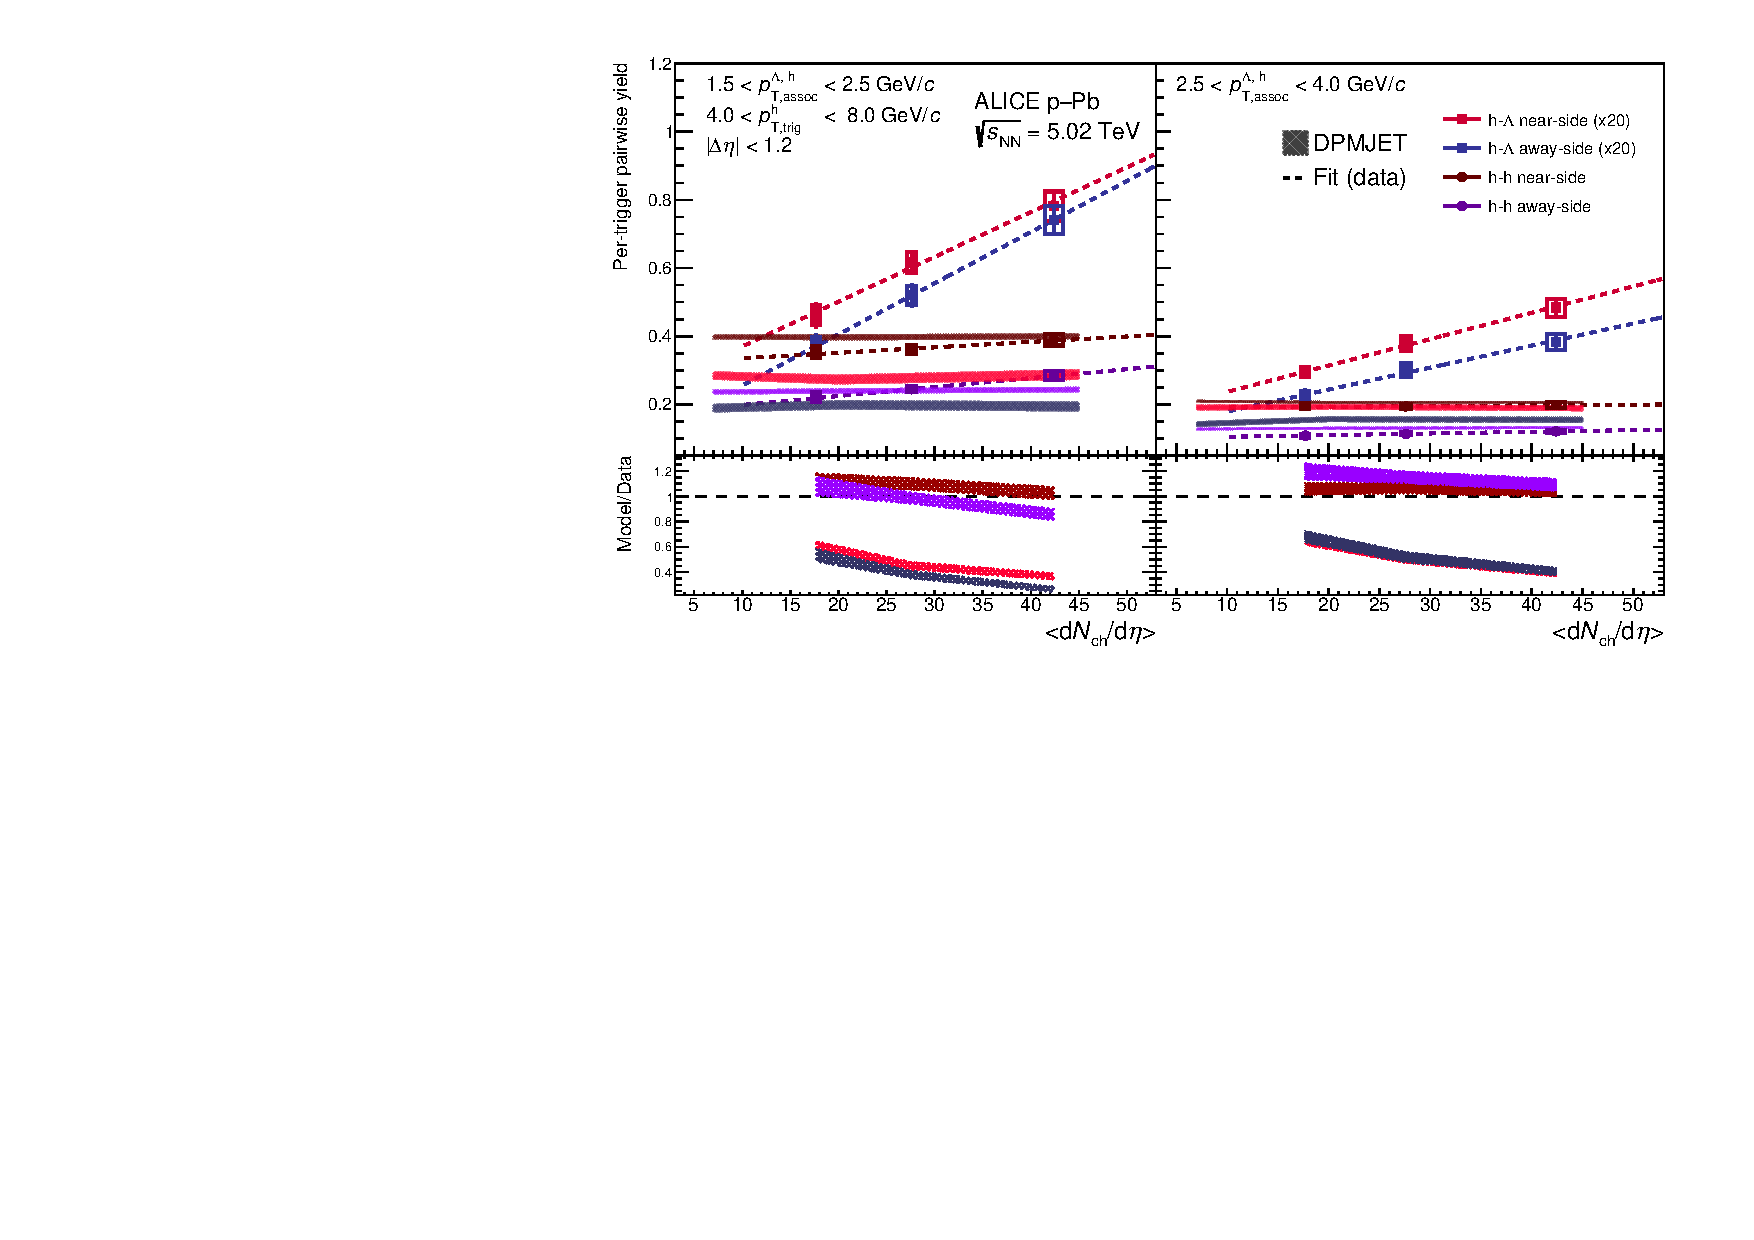
\includegraphics[width=\textwidth]{figures/results/final_pairwise_plot_new_x_axis_model_ratio.pdf}
\caption{The per-trigger pair-wise yields $Y_{\text{near}}, Y_{\text{away}}$ as a function of charged particle multiplicity for the h-$\Lambda$ (square markers) and h-h (circle markers) correlations in the lower (left) and higher (right) associated \pt ranges. The statistical (systematic) uncertainties are shown as vertical lines (boxes), and a first order polynomial fit to the data is shown as a dashed line. The same yields predicted by DPMJET are also shown as shaded bands, with the width of the band representing the systematic uncertainty on the model. The ratio of the model to the data is shown in the bottom panel, along with a dashed line drawn at unity.}
\label{fig:pairwise_yield}
\end{figure}

Across both associated \pt ranges, the h-$\Lambda$ yields see a substantial increase with respect to multiplicity for both the near- and away-side regions. This is in stark contrast to the dihadron yields, which see no significant increase as a function of multiplicity in both associated \pt ranges. The increase can be quantified by calculating the percent change in the per-trigger yields from the lowest to highest multiplicity class, which is shown for each momentum range in Table \ref{tab:percent_increase}. The errors reported are calculated using both the systematic and statistical uncertainties summed in quadrature, and the significance is obtained by calculating the deviation in the percent change from zero in terms of the total error. The significance obtained from the h-$\Lambda$ yields across both regions and \pt ranges are all $>2\sigma$, indicating that the increase is statistically significant. However, the dihadron yields see no statistically significant increase in both regions across both momentum ranges. In the h-\lmb and h-h cases, the percent changes in the away-side yields are systematically higher than the changes in the near-side yields. These differences between the near- and away-side yields' behavior as a function of multiplicity hint at a possible modification of the away-side jet production due to soft scattering.

\begin{table}
\centering
\caption{The percent change in the per-trigger yields from the lowest to highest multiplicity class in the lower and higher associated momentum ranges. The errors reported are obtained using the systematic and statistical uncertainties summed in quadrature. The reported significance is the number of standard deviations away from zero percent change.}
\begin{tabular}{l c c}
\hline
Region & Percent change for lower (higher) $p_{\text{T, assoc}}^{\text{h,}\Lambda}$ & Lower (higher) $p_{\text{T, assoc}}^{\text{h,}\Lambda}$ significance \\
\hline
h-$\Lambda$ near-side &  $47.9 \pm 16.8$ ($46.6 \pm 14.6$) & $ 2.9\sigma (3.2\sigma) $\\ 
h-$\Lambda$ away-side &  $71.0 \pm 22.5$ ($46.2 \pm 17.9$) & $3.2\sigma (2.6\sigma)$ \\
h-h near-side &  $ 0.4 \pm 7.5$ ($-3.9 \pm 4.3$) & $0.1\sigma (-0.9\sigma)$ \\
h-h away-side &  $11.7 \pm 12.3$ ($1.0 \pm 7.0$) & $0.9\sigma (0.1\sigma)$ \\
\hline
\end{tabular}
\label{tab:percent_increase}
\end{table}

The per-trigger near- and away-side yields predicted by DPMJET are mostly consistent with data in the dihadron case. This can be seen in the model/data ratio, with both the near- and away-side ratios remaining close to unity across the entire multiplicity range. The h-$\Lambda$ yields, however, are not well described by the model. Both the near- and away-side h-$\Lambda$ yields predicted by DPMJET are lower than data by around a factor of two across the entire multiplicity range in both momentum ranges, and there is no significant increase in these yields as a function of multiplicity. 

To gain more insight to the underlying mechanisms responsible for strangeness production in jets, the widths of the near- and away-side peak regions are extracted from the h-$\Lambda$ and h-h $\Delta\varphi$ distributions using Equations \ref{eq:fullfit} and \ref{eq:width}. Plots of these widths as a function of multiplicity for both associated momentum ranges are shown in Figure \ref{fig:jet_widths}, along with the same widths predicted by DPMJET. A ratio of the model to the data is also presented in the bottom panel of the figure.

\begin{figure}[h!]
\centering
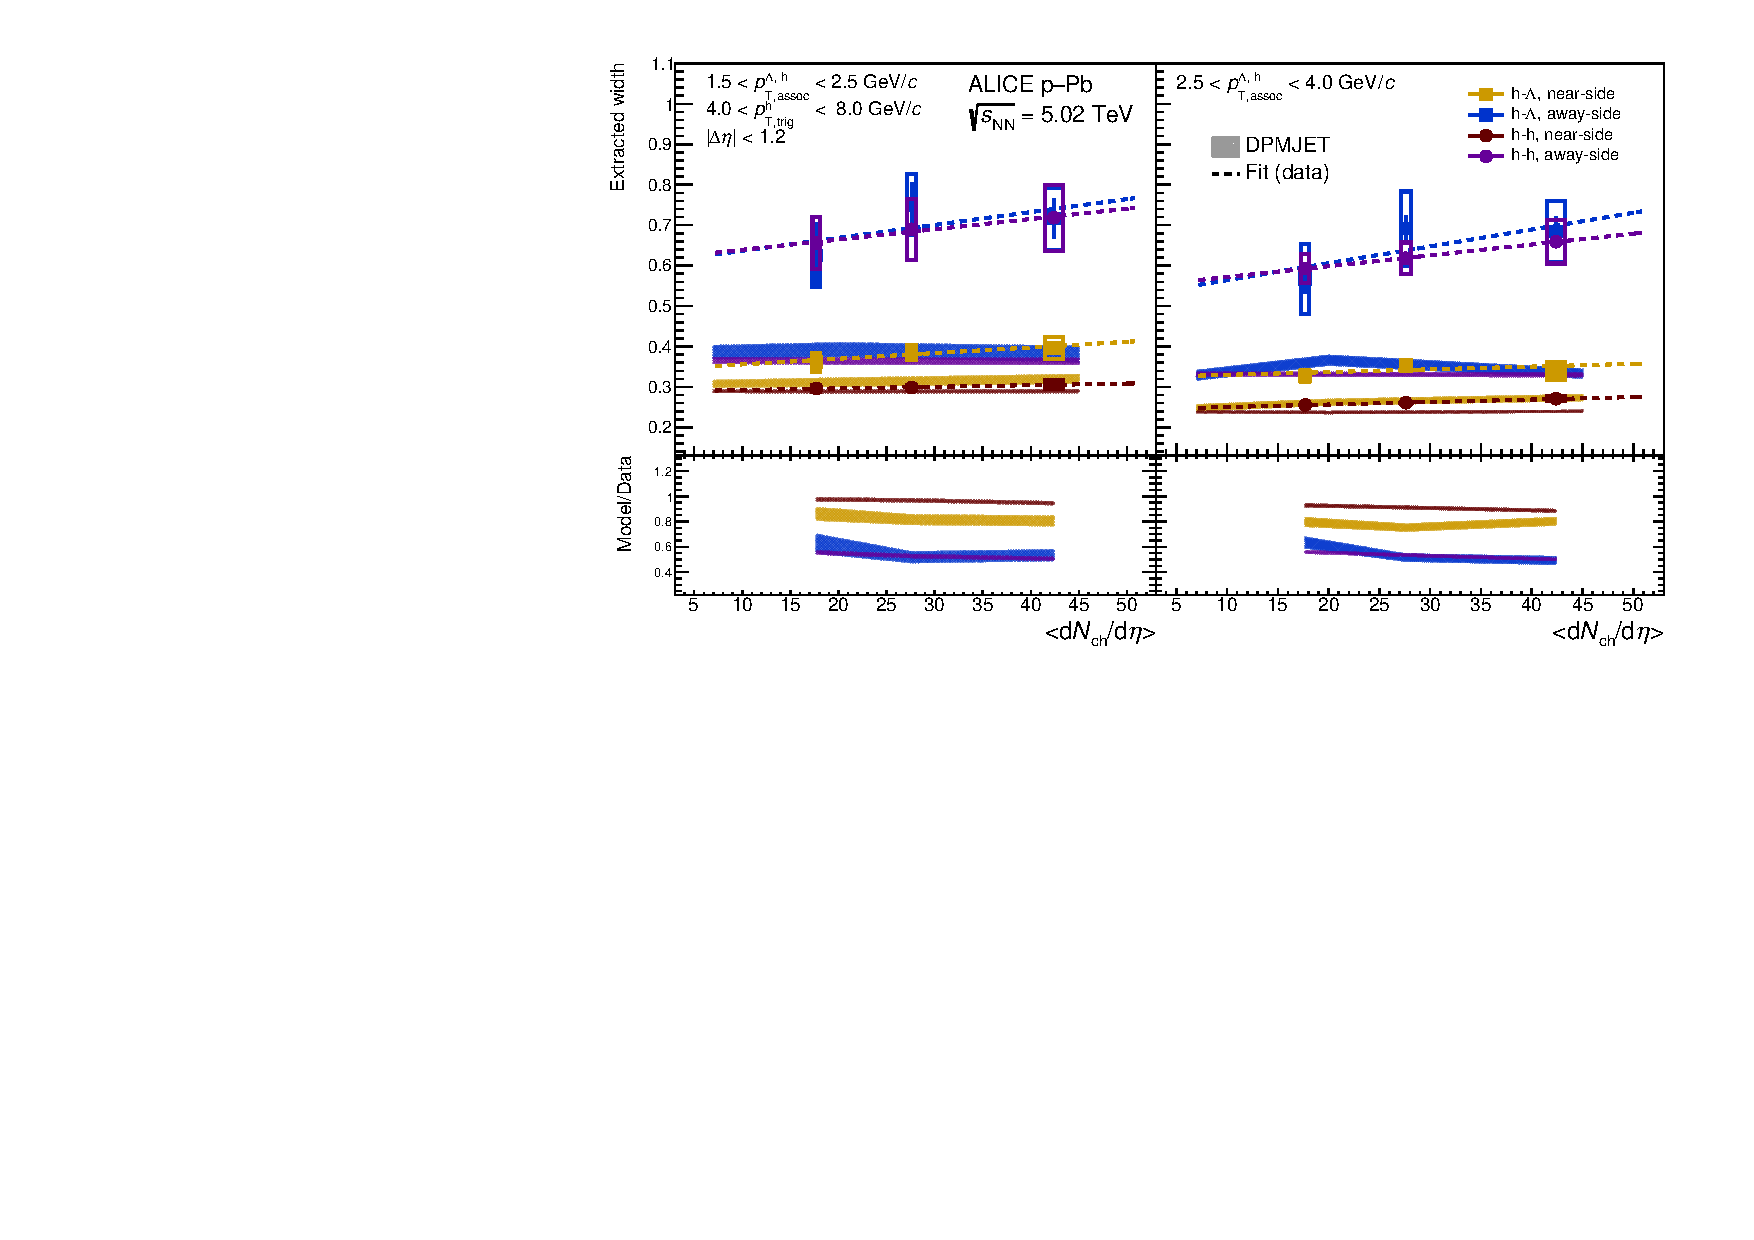
\includegraphics[width=\textwidth]{figures/results/final_width_plot_new_x_axis_model_ratio.pdf}
\caption{The h-$\Lambda$ and h-h near- and away-side peak widths shown as a function of multiplicity for both associated momentum ranges, along with a straight-line fit to the data. The statistical (systematic) uncertainties are shown as vertical lines (boxes). The ratios predicted by DPMJET are also presented as shaded bands, with the width of the band represending the systematic uncertainty on the model. The ratio of the model to the data is presented in the bottom panel, along with a dashed line drawn at unity.}
\label{fig:jet_widths}
\end{figure}


Expectedly, the near-side widths exhibit a significant decrease ($>$15\%) from the lower momentum range to the higher for both the h-$\Lambda$ and h-h cases, indicating that higher momentum associated particles are more collimated along the jet axis. An interesting result comes from comparing the h-$\Lambda$ and h-h away-side peak widths in data, which are found to be the same within systematic uncertainties across all multiplicity and momentum ranges, although the uncertainties are very large. This contrasts with the h-$\Lambda$ near-side widths, which are around 40\% ($2\sigma$) larger than the h-h widths across the entire multiplicity range for both momentum ranges. For the h-h near-side widths, DPMJET describes the data well across both momentum ranges, with a $<5 (10)$\%  deviation from data seen in the lower (higher) momentum range. DPMJET also predicts the h-$\Lambda$ near-side width to be larger than the h-h width, though the values of the h-$\Lambda$ widths are much lower than they are in data. One explanation for these differences between the near-side widths could be due the presence of gluon jets, which are generally more wide than quark jets ~\cite{GluonJet1} and exhibit an increased production of $\Lambda$ baryons ~\cite{GluonJet2}. As DPMJET includes both quark and gluon jets, it is possible that the predicted differences between the h-$\Lambda$ and h-h near- and away-side peak widths are due to this effect. 

DPMJET also under-predicts both the h-$\Lambda$ and h-h away-side widths by around 40\% across both momentum ranges. As the DPMJET model does not include any medium effects, this suggests that the away-side peak widths in data are possibly ``broadened'' by jet-medium interactions. However, the larger uncertainties on the away-side widths prevent the exclusion of flat behavior with respect to multiplicity (i.e. increasing medium size), as the slopes are all consistent with zero within uncertainties.





\subsection{Per-trigger yield ratios}

To better understand the differences between $\Lambda$ and charged hadron production both in and out-of jets, the per-trigger yield ratios $R_{i}^{\Lambda/h} \equiv Y_{i}^{h-\Lambda}$/$Y_{i}^{h-h}$ ($i$ = near-side, away-side, UE) are measured as a function of multiplicity in both associated momentum ranges. These ratios serve as a proxy for the $\Lambda/\pi$ ratio in each region, and are shown in Figure \ref{fig:lambda_hadron_ratio}. Straight line fits to the data are shown as dashed lines, with slopes and corresponding errors reported in Table \ref{tab:lambda_hadron_slopes}. The same ratios predicted by DPMJET are again shown, with a ratio to the data presented in the bottom panel. 

\begin{figure}[h!]
\centering
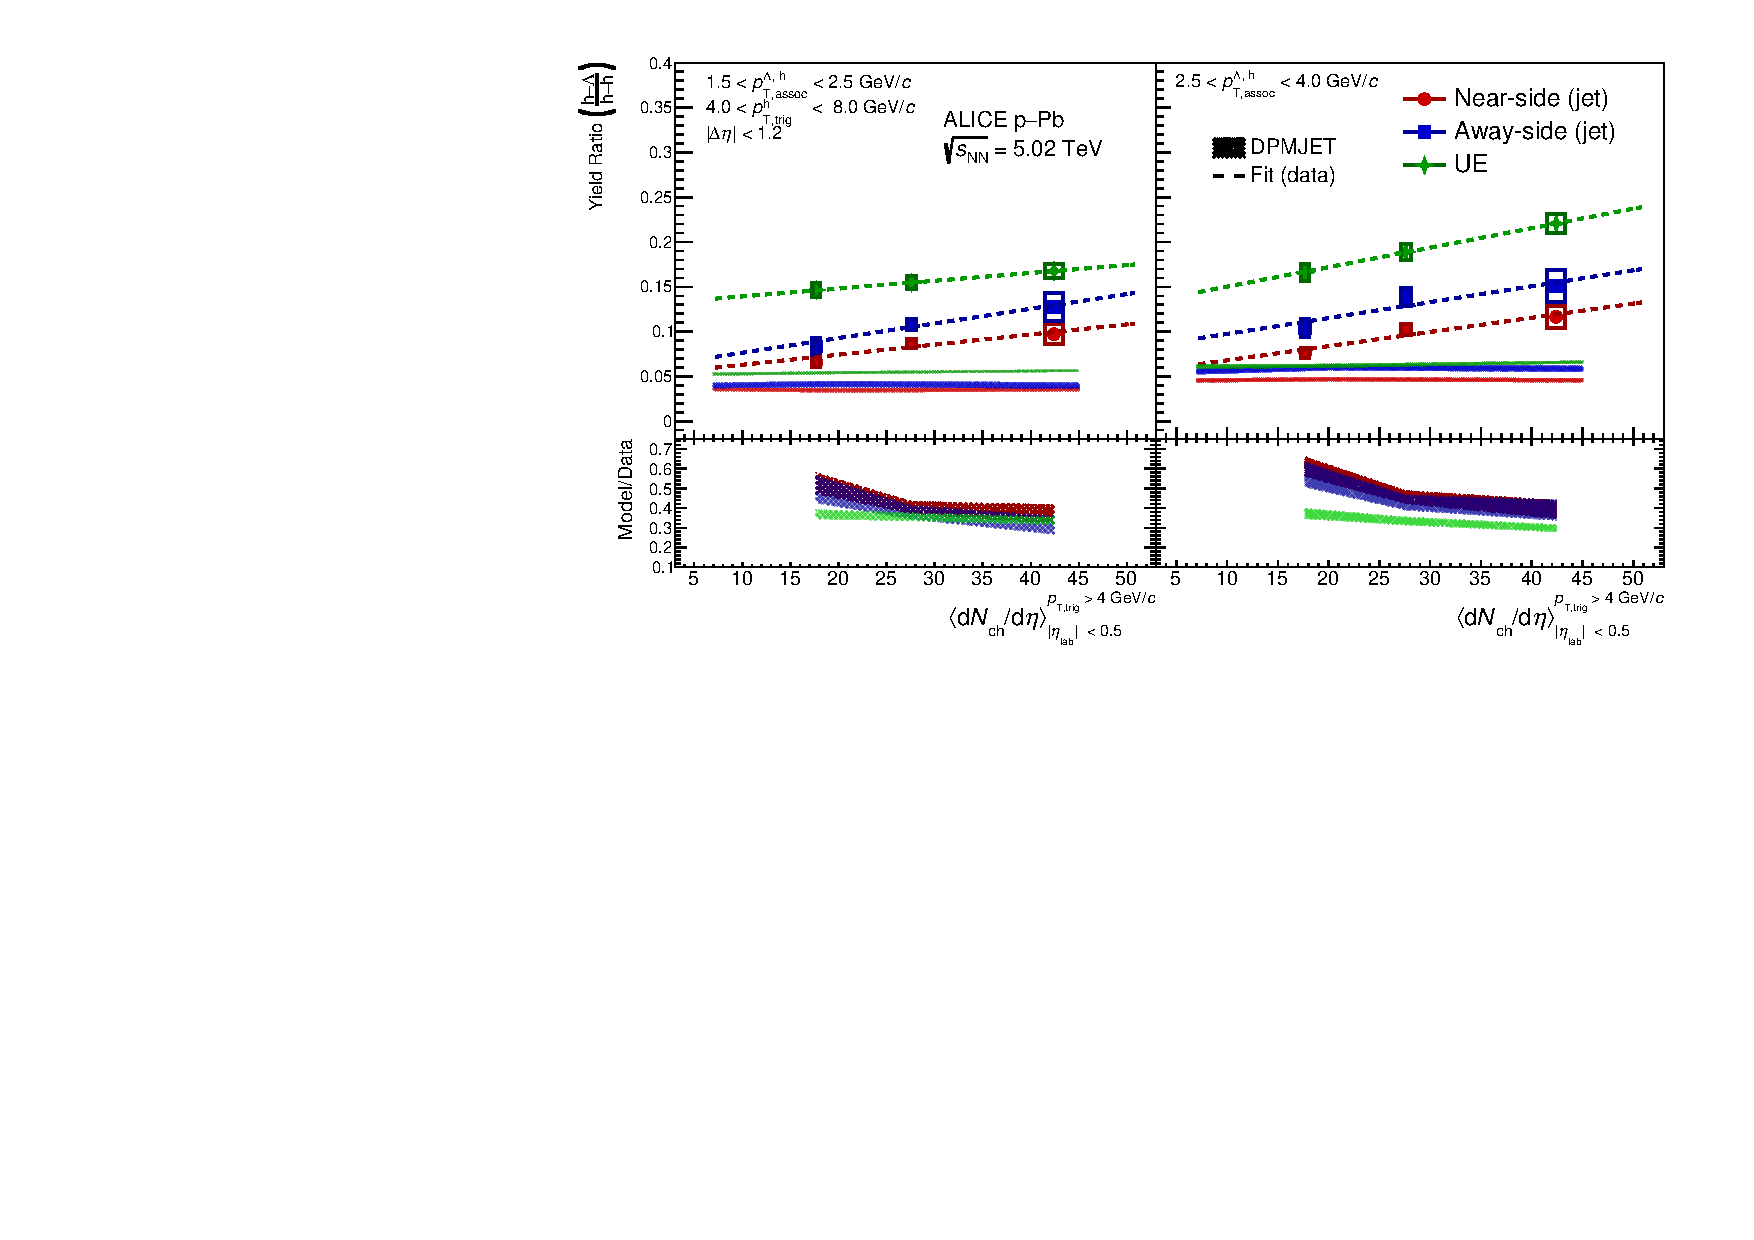
\includegraphics[width=\textwidth]{figures/results/final_lambda_hadron_ratio_plot_new_x_axis_model_ratio.pdf}
\caption{The per-trigger pair-wise yield ratios $R_{i}^{\Lambda/h} \equiv Y_{i}^{h-\Lambda}$/$Y_{i}^{h-h}$ ($i$ = near-side, away-side, UE) as a function of multiplicity in the lower (left) and higher (right) associated momentum ranges. The statistical (systematic) uncertainties are shown as vertical lines (boxes). The ratios predicted by DPMJET are also presented as shaded bands, with the width of the band represending the systematic uncertainty on the model. The ratio of the model to the data is presented in the bottom panel.}
\label{fig:lambda_hadron_ratio}
\end{figure}

One surprising feature of these results is the clear separation between the ratios in each region across the entire multiplicity range in both momentum ranges, with the UE ratio being the largest, followed by the away-side ratio, and finally the near-side. This indicates that most of the relative $\Lambda$ production is occuring in the UE, which is consistent with the idea that $s$-quark production is maximal in the medium. This is further supported by the fact that the away-side ratio is larger than the near-side, as $\Lambda$ production on the away-side is likely due to both the fragementation of the away-side jet coupled with the possible production of strange quarks due to jet-medium interactions. Interestingly, DPMJET is able to produce this ordering in the ratios, but the magnitude of the ratios is not well described. 

\begin{table}
\centering
\caption{The slopes obtained from the straight-line fits to the per-trigger pair-wise (h-$\Lambda$)/(h-h)yield ratios as a function of multiplicity in both associated momentum ranges. The fits are made using the statistical and systematic errors summed in quadrature. All fits are such that $\chi^{2}/\text{ndf} < 1$.}
\begin{tabular}{l c c}
\hline
Region & Lower $p_{\text{T, assoc}}^{\text{h,}\Lambda}$ slope ($\times10^{-3}$) & Higher $p_{\text{T, assoc}}^{\text{h,}\Lambda}$  slope ($\times10^{-3}$) \\
\hline
Near-side & $1.1 \pm 0.4$ & $1.6 \pm 0.4$ \\
Away-side & $1.6 \pm 0.6$ & $1.8 \pm 0.7$ \\
UE & $0.9 \pm 0.1$ & $2.2 \pm 0.2$ \\
\hline
\end{tabular}
\label{tab:lambda_hadron_slopes}
\end{table}


The near- and away-side slopes reported in Table \ref{tab:lambda_hadron_slopes} are all more than $2\sigma$ greater than zero, indicating that there is an enhancement of relative $\Lambda$ production in jets as a function of multiplicity. This result is consistent with previous measurements of the $\phi(1020)$ meson in jets ~\cite{JustinPaper}, where a similar enhancement of the $\phi$/h ratio is observed in the near- and away-side regions. This provides further evidence that the production of strange quarks is enhanced in jets. The away-side slopes are also systematically larger than the near-side slopes in both momentum ranges, again hinting at possible modification of the away-side $s$-quark production due to jet-medium interactions. Similarly, the UE slopes are not compatible with zero, but the value is smaller than the near- and away-side slopes by about $1\sigma$ in the lower momentum range. However, the larger values of the UE ratios overall still suggest that a significant portion of the observed enhancement in the $\Lambda$/$\pi$ ratio is due to softer production from the UE. The slopes calculated using the ratios obtained from DPMJET are all nearly exactly zero, and are thus not shown in the table.



\subsection{Comparison with the $\phi(1020)$}

The $\phi(1020)$ meson's net strangeness $|S|$ is equal to zero. Despite this, it has been observed to exhibit a similar enhancement in production as a function of multiplicity as other hadrons with non-zero strangeness ~\cite{PhiEnhancement}. Due to their similar masses ($\Delta M < 100$ \MeVmass), the $\phi(1020)$ is an excellect candidate to compare directly with the $\Lambda$ in order to better understand the differences between open ($|S| \neq 0$) and hidden ($|S| = 0$) strange hadron production. Using previously published results on $\phi(1020)$ production in and out-of jets in \pPb collisions at $\sqrt{s_{\text{NN}}} = 5.02$ \TeV ~\cite{JustinPaper}, the per-trigger pair-wise yield ratios $R_{i}^{\Lambda/\phi} \equiv Y_{i}^{h-\Lambda}/Y_{i}^{h-\phi}$ ($i$ = near-side, away-side, UE) can be measured as a function of multiplicity, which are shown in Figure \ref{fig:lambda_phi_ratio} for both the lower and higher associated \pt ranges. Again, straight line fits to the data are shown as a dashed lines, with the slopes and corresponding errors reported in Table \ref{tab:lambda_phi_slopes}. The same ratios predicted by DPMJET are also presented, with a ratio to the data presented in the bottom panel.


\begin{figure}[h!]
\centering
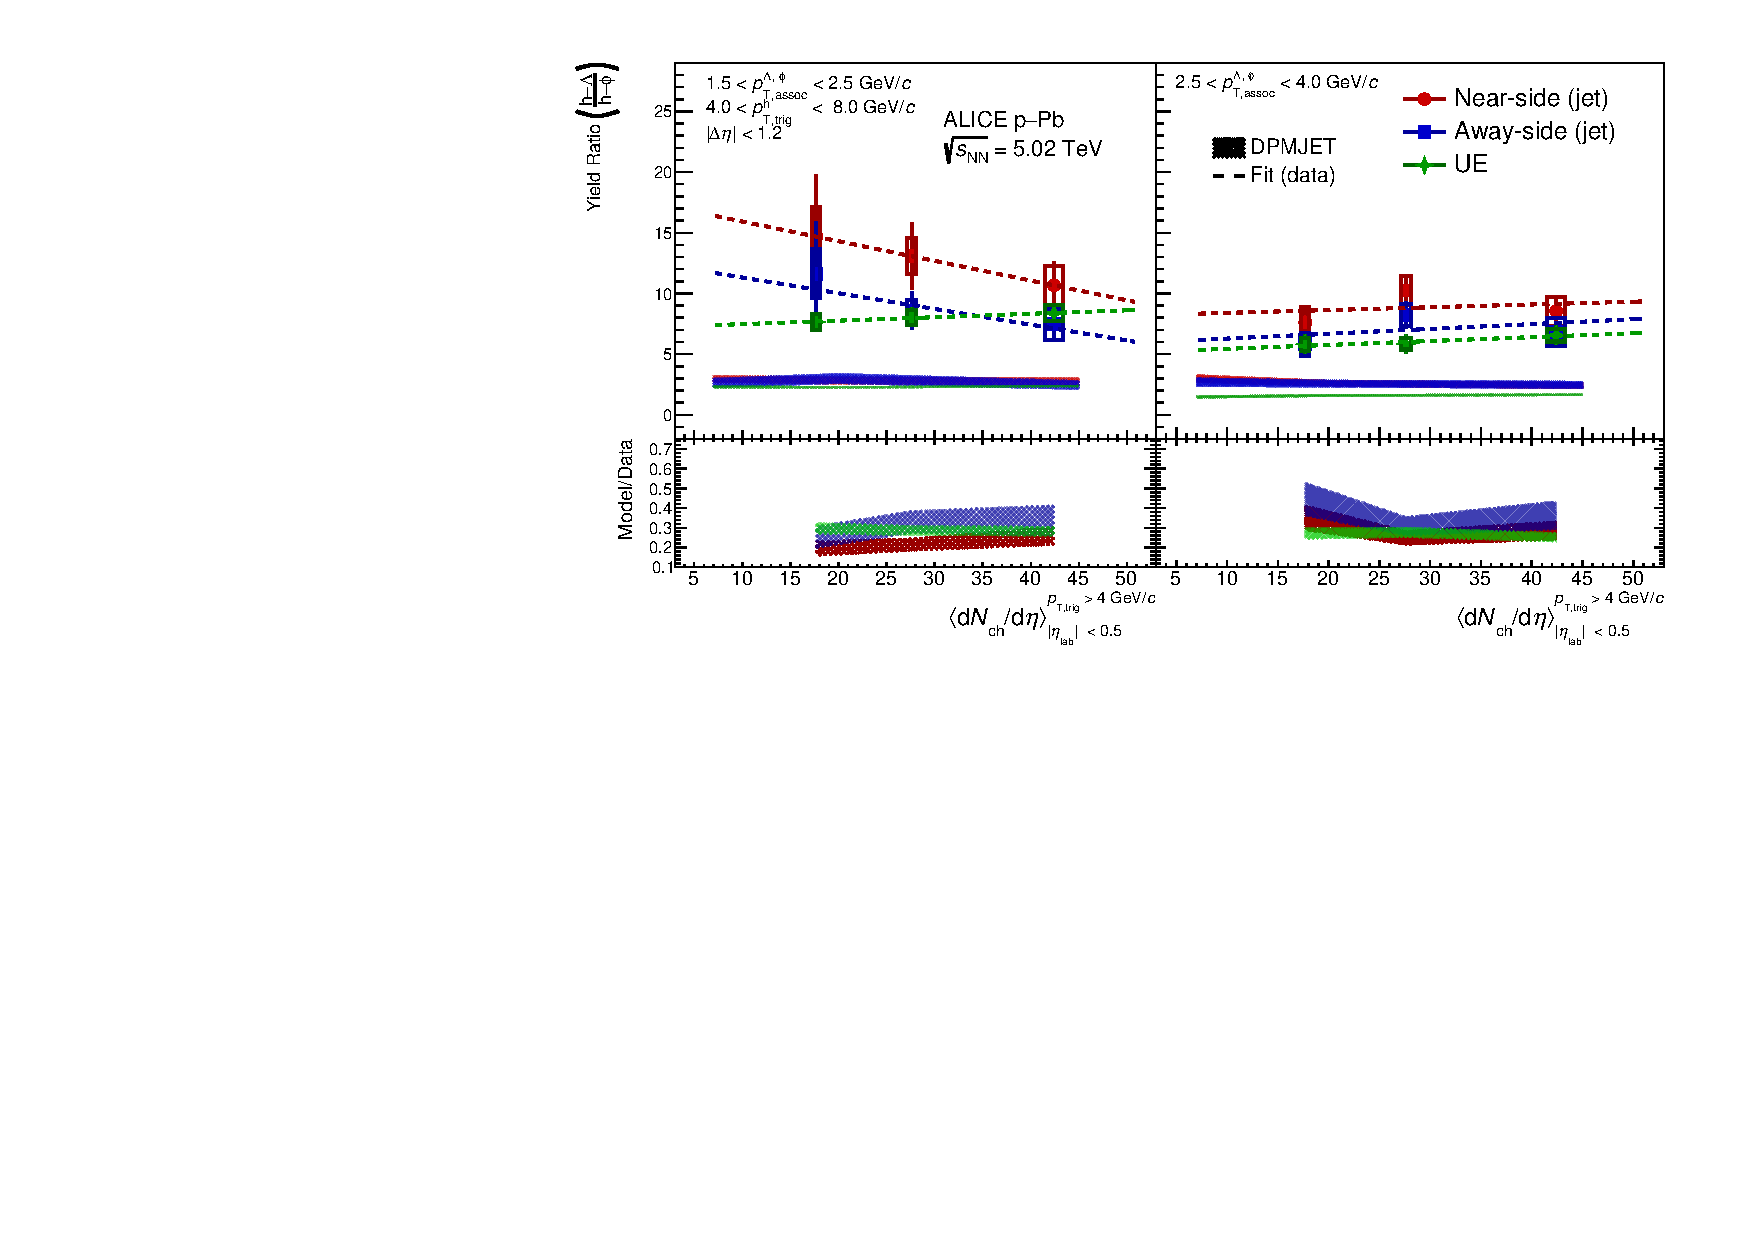
\includegraphics[width=\textwidth]{figures/results/final_lambda_phi_ratio_plot_new_x_axis_model_ratio.pdf}
\caption{The per-trigger pair-wise yield ratios $R_{i}^{\Lambda/\phi} \equiv Y_{i}^{h-\Lambda}$/$Y_{i}^{h-\phi}$ ($i$ = near-side, away-side, UE) as a function of multiplicity in the lower (left) and higher (right) associated momentum ranges. The statistical (systematic) uncertainties are shown as vertical lines (boxes).  The ratios predicted by DPMJET are also presented as shaded bands, with the width of the band represending the systematic uncertainty on the model. The ratio of the model to the data is presented in the bottom panel.}
\label{fig:lambda_phi_ratio}
\end{figure}

Interestingly, $\Lambda/\phi$ near-side ratios are systematically higher than the ratios in all other regions across the entire multiplicity range and both momentum ranges. This indicates relative enhancement (supression) of $\Lambda$ ($\phi$) production along the jet axis. As strangeness is always produced in the form of $s\bar{s}$ pairs, one possible explanation of this effect is that when these pairs are produced from jet fragmentation, the $s$ and $\bar{s}$ are less likely to hadronize into the same $\phi$ due to their separation in phase-space. The away-side ratios are higher than the UE ratios on average, but the difference is not as pronounced as in the near-side.  The ratios predicted by DPMJET provide further evidence for this explanation, as the model shows the near- and away-side ratios are systematically higher than the UE ratios across the entire multiplicity range. However, DPMJET predicts no differences between the near- and away-side $\Lambda$/$\phi$ ratios, possibly due to the missing medium effects in the model. While the central values of the near- and away-side ratios in the lower associated momentum range decrease with increasing multiplicity, the uncertainties are very large. All of the slopes presented in Table \ref{tab:lambda_phi_slopes} are compatible with zero, indicating no dependence on multiplicity for the $\Lambda$/$\phi$ ratios.

\begin{table}
\centering
\caption{The slopes obtained from the straight-line fits to the per-trigger pair-wise (h-$\Lambda$)/(h-$\phi$) yield ratios as a function of multiplicity in both associated momentum ranges. The fits are made using the statistical and systematic errors summed in quadrature. All fits are such that $\chi^{2}/\text{ndf} < 1$.}
\begin{tabular}{l c c}
\hline
Region & Lower $p_{\text{T, assoc}}^{\Lambda, \phi}$ slope ($\times10^{-1}$) & Higher $p_{\text{T, assoc}}^{\Lambda, \phi}$ slope ($\times10^{-1}$) \\
\hline
Near-side & $ -1.6\pm 2.0$ & $0.2 \pm 0.9$ \\
Away-side & $ -1.1 \pm 1.4$ & $0.3 \pm 0.7$ \\
UE & $0.3 \pm 0.4$ & $0.3 \pm 0.3$ \\
\hline
\end{tabular}
\label{tab:lambda_phi_slopes}
\end{table}


\subsection{Model Comparisons}
\label{model_comparisons}
In this section, we detail how the results of this analysis in data compare to some of the best p--Pb model calculations. We consider the following models for comparison:
\begin{itemize}
\item \href{https://arxiv.org/pdf/hep-ph/0012252.pdf}{DPMJet} using LHC18f3
\item \href{https://arxiv.org/pdf/1306.0121.pdf}{EPOS-LHC} using LHC17f2a
\item \href{https://arxiv.org/pdf/0808.0022.pdf}{PHSD} through 200 million events generated using university computing resources
\end{itemize}

For each of these comparisons, we apply the same techniques and cuts as they were in data (if applicable). More explicitly, all of the following are kept the same:
\begin{itemize}
\item Event selection (require $>$ 2 charged hadrons at mid-rapidity)
\item Multiplicity percentile selection (using charged hadrons in V0A acceptance, more details in Section \ref{model_mult_percentiles})
\item Trigger and associated $\eta$ range ($|\eta| < 0.8$)
\item Trigger and associated $p_{T}$ ranges
\item $\Delta\eta$ range ($|\Delta\eta| < 1.2$)
\item $N_{bins}$ for $\Delta\varphi$ distributions (16 bins)
\end{itemize}

We do not apply any of the corrections we used in data (efficiency, two-track effects, etc.) to the models, as they are not required. However, we do apply the standard mixed-event correction procedure to all models except PHSD, whereby we simply remove the single-particle $\eta$ cut on the associated hadron to remove any geometric effects from finite acceptance. This is currently being investigated, as the $h-\Lambda$ 2D distributions in PHSD look a little strange...

\subsubsection{2D Angular Correlation Distributions}
\label{model_2d_correlations}

The multiplicity-integrated per-trigger $h-\Lambda$ and $h-h$ 2D $\Delta\eta\Delta\varphi$ distributions in data and for each model can be seen in Figures \ref{h_lambda_2d_model} ($h-\Lambda$) and \ref{h_h_2d_model} ($h-h$). We also show the $h-\phi$ distributions for each model in Figure \ref{h_phi_2d_model}, but the multiplicity-integrated data is unavailable. While these distributions are never used directly in this analysis, they reveal interesting features of each of the models. 

For the dihadron correlations, we see zero flow effects with DPMJet, whereas EPOS-LHC massively overestimates the $v_{2}$, with the away-side jet contribution being nearly washed out. PHSD appears to be a nice middleground between the two, with a nearly identical shape to the data (though the per-trigger yield is quite a bit smaller).

For the $h-\Lambda$ correlations, we again see that there is no $v_{2}$ with DPMJet whereas EPOS-LHC has so much flow that even the near-side jet peak is barely visible. PHSD no longer appears to be a nice middle ground, as there is now a dome-like structure across $\Delta\eta$ that was not present in the dihadron case. 

The $h-\phi$ distributions tell a similar story as the $h-\Lambda$ distributions, with DPMJet having no flow and EPOS-LHC having too much flow. It also appear as if PHSD is massively underestimating the per-trigger $\phi$ production, which requires investigation.


\begin{figure}[ht]
\centering
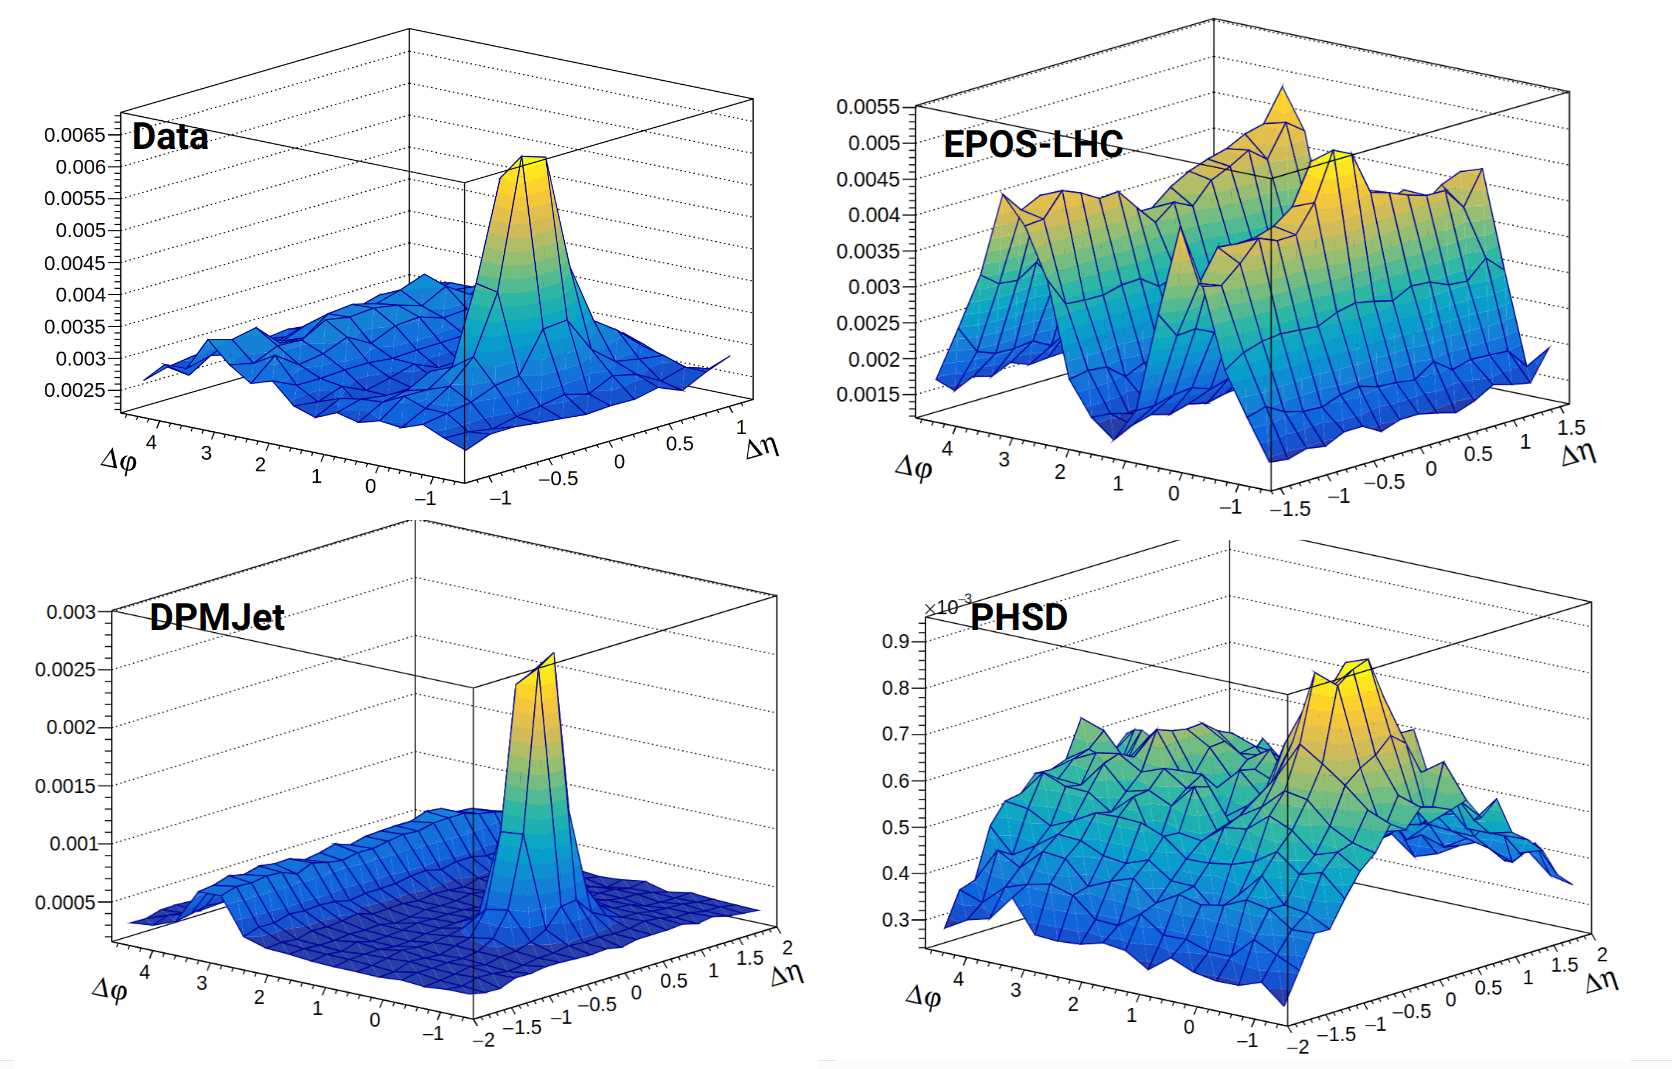
\includegraphics[width=5in]{figures/h_lambda_2d_modelcomp.png}
\caption{The multiplicity-integrated per-trigger $h-\Lambda$ 2D $\Delta\eta\Delta\varphi$ distributions in data and for each model within our central associated $p_{T}$ bin (2.0 - 4.0 GeV/c).}
\label{h_lambda_2d_model}
\end{figure}

\begin{figure}[ht]
\centering
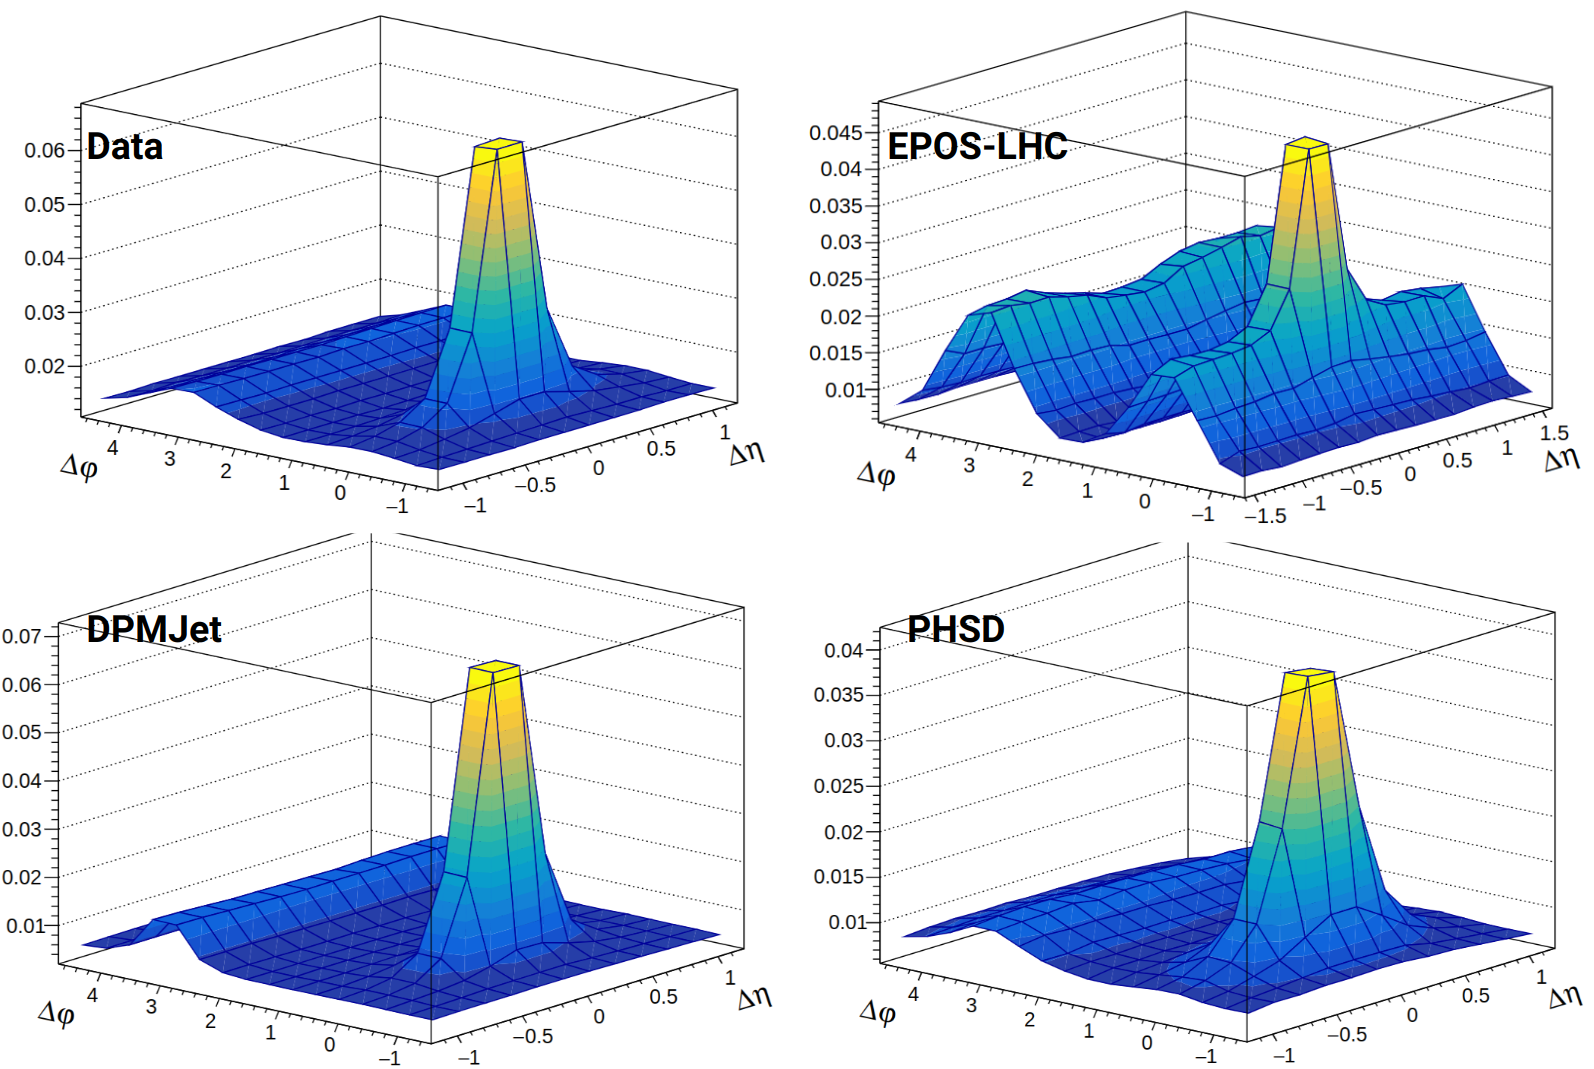
\includegraphics[width=5in]{figures/h_h_2d_modelcomp.png}
\caption{The multiplicity-integrated per-trigger $h-h$ 2D $\Delta\eta\Delta\varphi$ distributions in data and for each model within our central associated $p_{T}$ bin (2.0 - 4.0 GeV/c).}
\label{h_h_2d_model}
\end{figure}
\clearpage

\begin{figure}[ht]
\centering
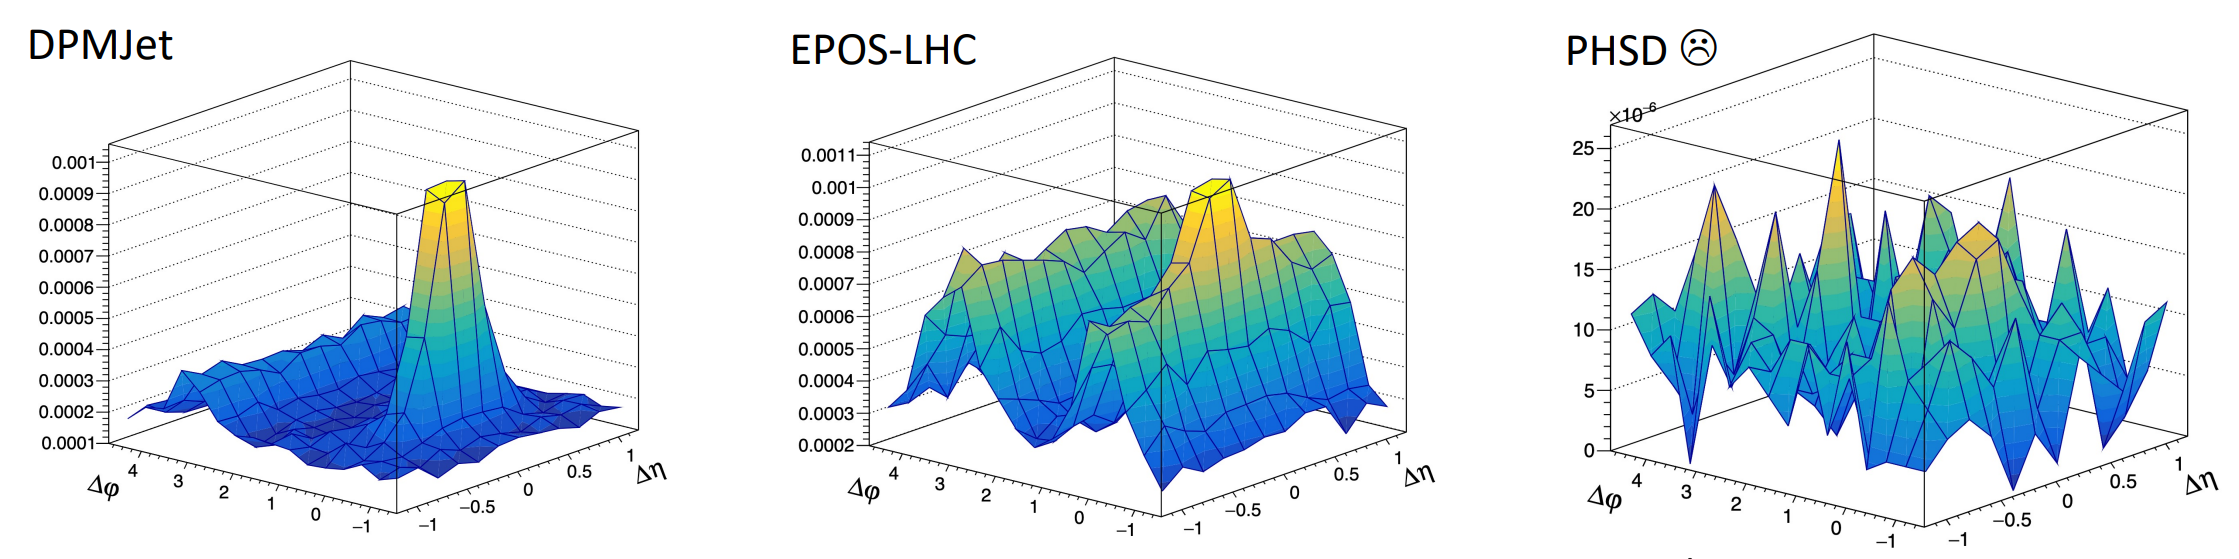
\includegraphics[width=6in]{figures/h_phi_2d_modelcomp.png}
\caption{The multiplicity-integrated per-trigger $h-\phi$ 2D $\Delta\eta\Delta\varphi$ distributions for each model within our central associated $p_{T}$ bin (2.0 - 4.0 GeV/c).}
\label{h_phi_2d_model}
\end{figure}

\subsubsection{1D $\Delta\varphi$ Correlation Distributions}
\label{model_1d_correlations}

The multiplicity-integrated per-trigger $h-\Lambda$ and $h-h$ $\Delta\varphi$ distribution fits in data and for each model can be seen in Figure \ref{1d_modelcomp}. Note that the underlying event has been subtracted off for each distribution, which was done by fitting the near-side of EPOS-LHC and PHSD in the outer ($|\Delta\eta| > 1.2$) region to the following function:
\begin{equation}
Fit_{v_{4}} = \sum_{i=0}^{4} a_{i}cos(i\Delta\varphi),
\end{equation}
and by the average of 6 non-jet-containing $\Delta\varphi$ bins (1, 2, 7, 8, 9, 16) in the case of DPMJet. An example of the dihadron underlying event fit can be seen in Figure \ref{epos_ue_fit}. In the $h-\Lambda$ case, we are unable to generate fits for EPOS-LHC due to the fact that the underlying event subtraction procedure creates too much noise on the away-side of the distribution.

\begin{figure}[ht]
\centering
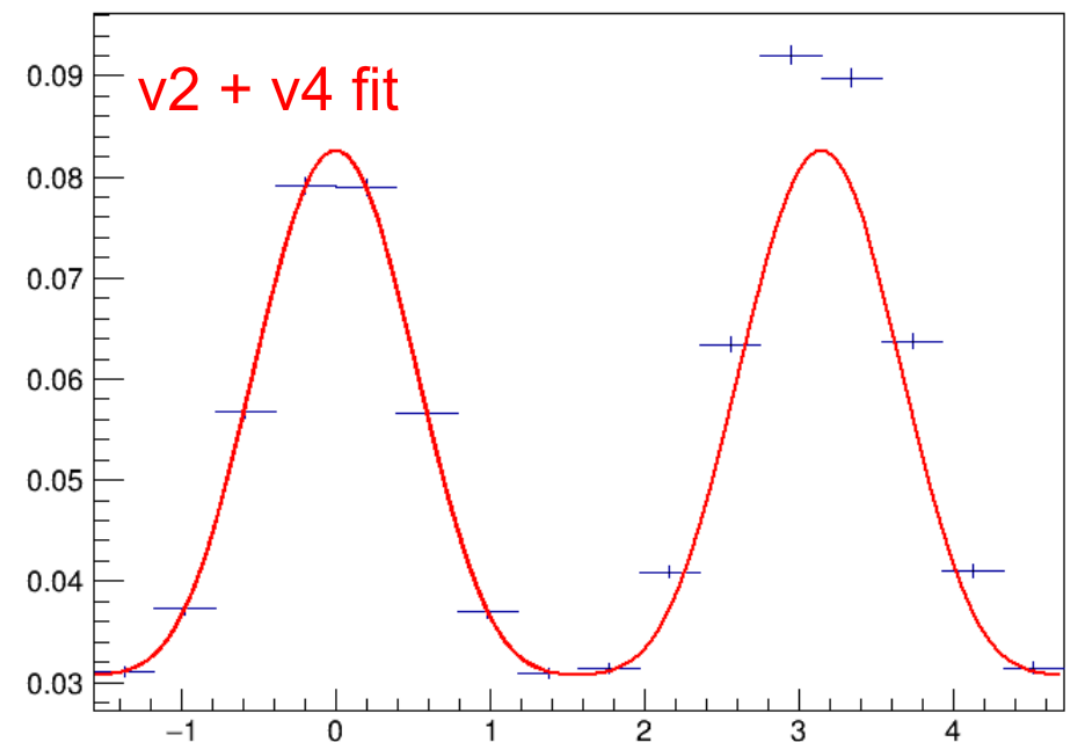
\includegraphics[width=4in]{figures/epos_ue_fit.png}
\caption{An example of the underlying event fit for EPOS-LHC in the dihadron case, taken in the $|\Delta\eta| > 2$ range. Note that even though the $v_1$ and $v_3$ terms were allowed to vary, they were consistent with zero.}
\label{epos_ue_fit}
\end{figure}

For the $h-\Lambda$ distributions, we see that both DPMJet and PHSD underestimate the near- and away-side jet yields, with PHSD being much lower than DPMJet. We also observe that DPMJet appears to underestimate the away-side width, whereas PHSD ``overestimates'' it (though the away-side is barely present in the first place).

In the dihadron case, we see that no models are able to completely describe the shape of the distribution from data. DPMJet overestimates the near- and away-side peaks, whereas EPOS-LHC underestimates them. PHSD also underestimates the jet-like peaks, but is closer to the data than EPOS-LHC.

\begin{figure}[ht]
\centering
\begin{subfigure}{
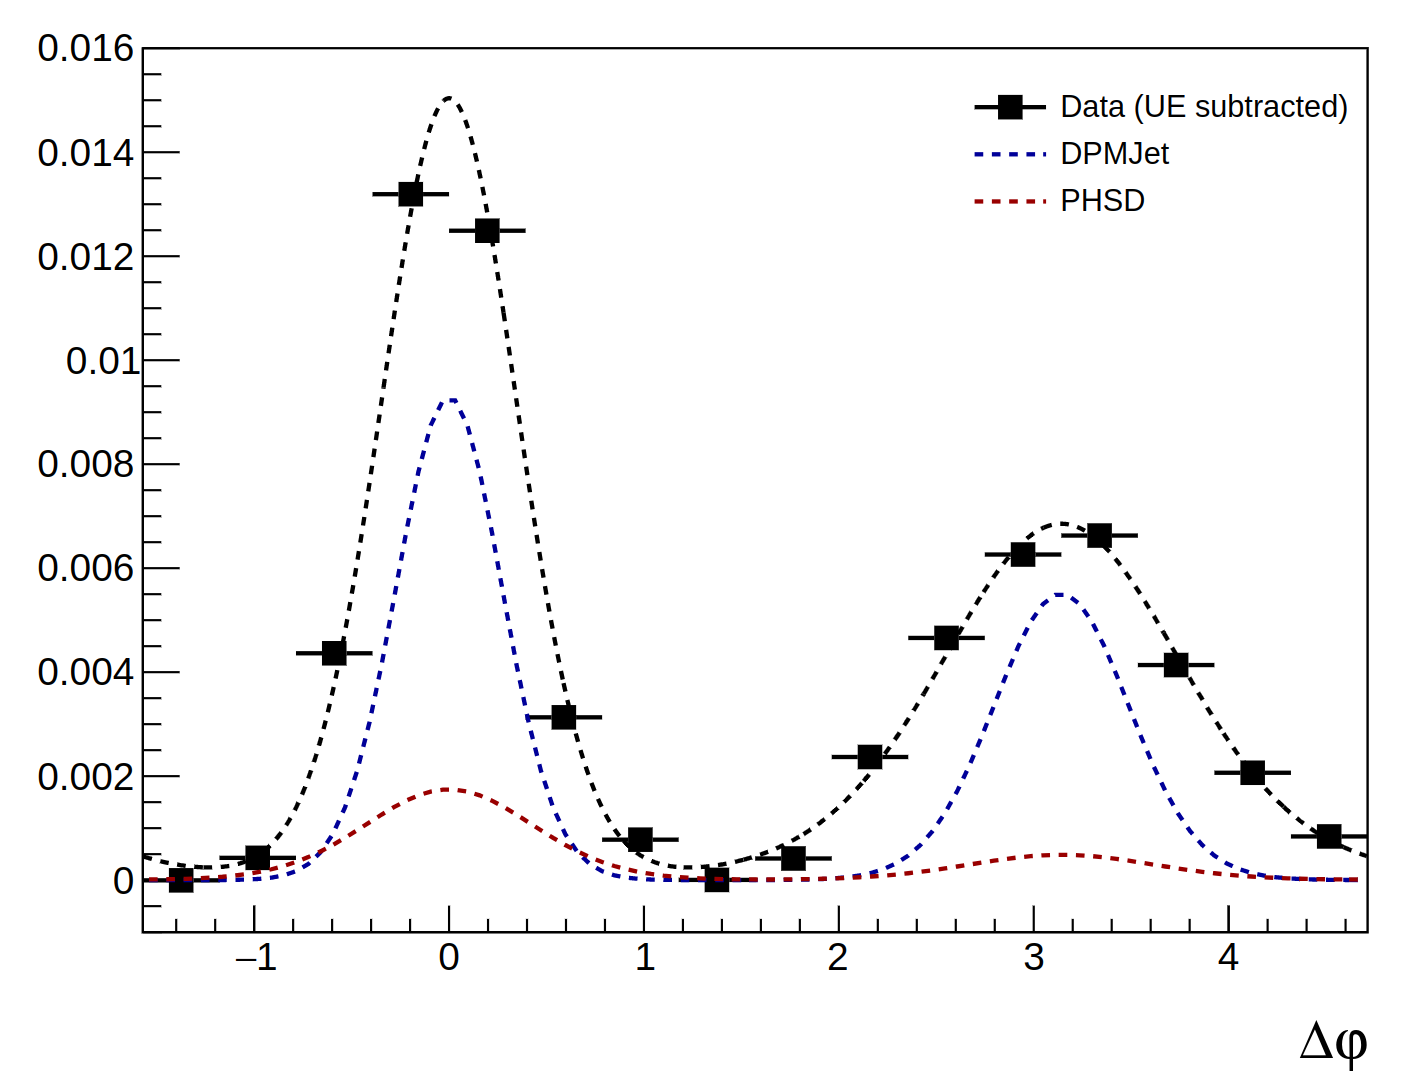
\includegraphics[width=3in]{figures/h_lambda_1d_modelcomp.png}}
\end{subfigure}
\begin{subfigure}{
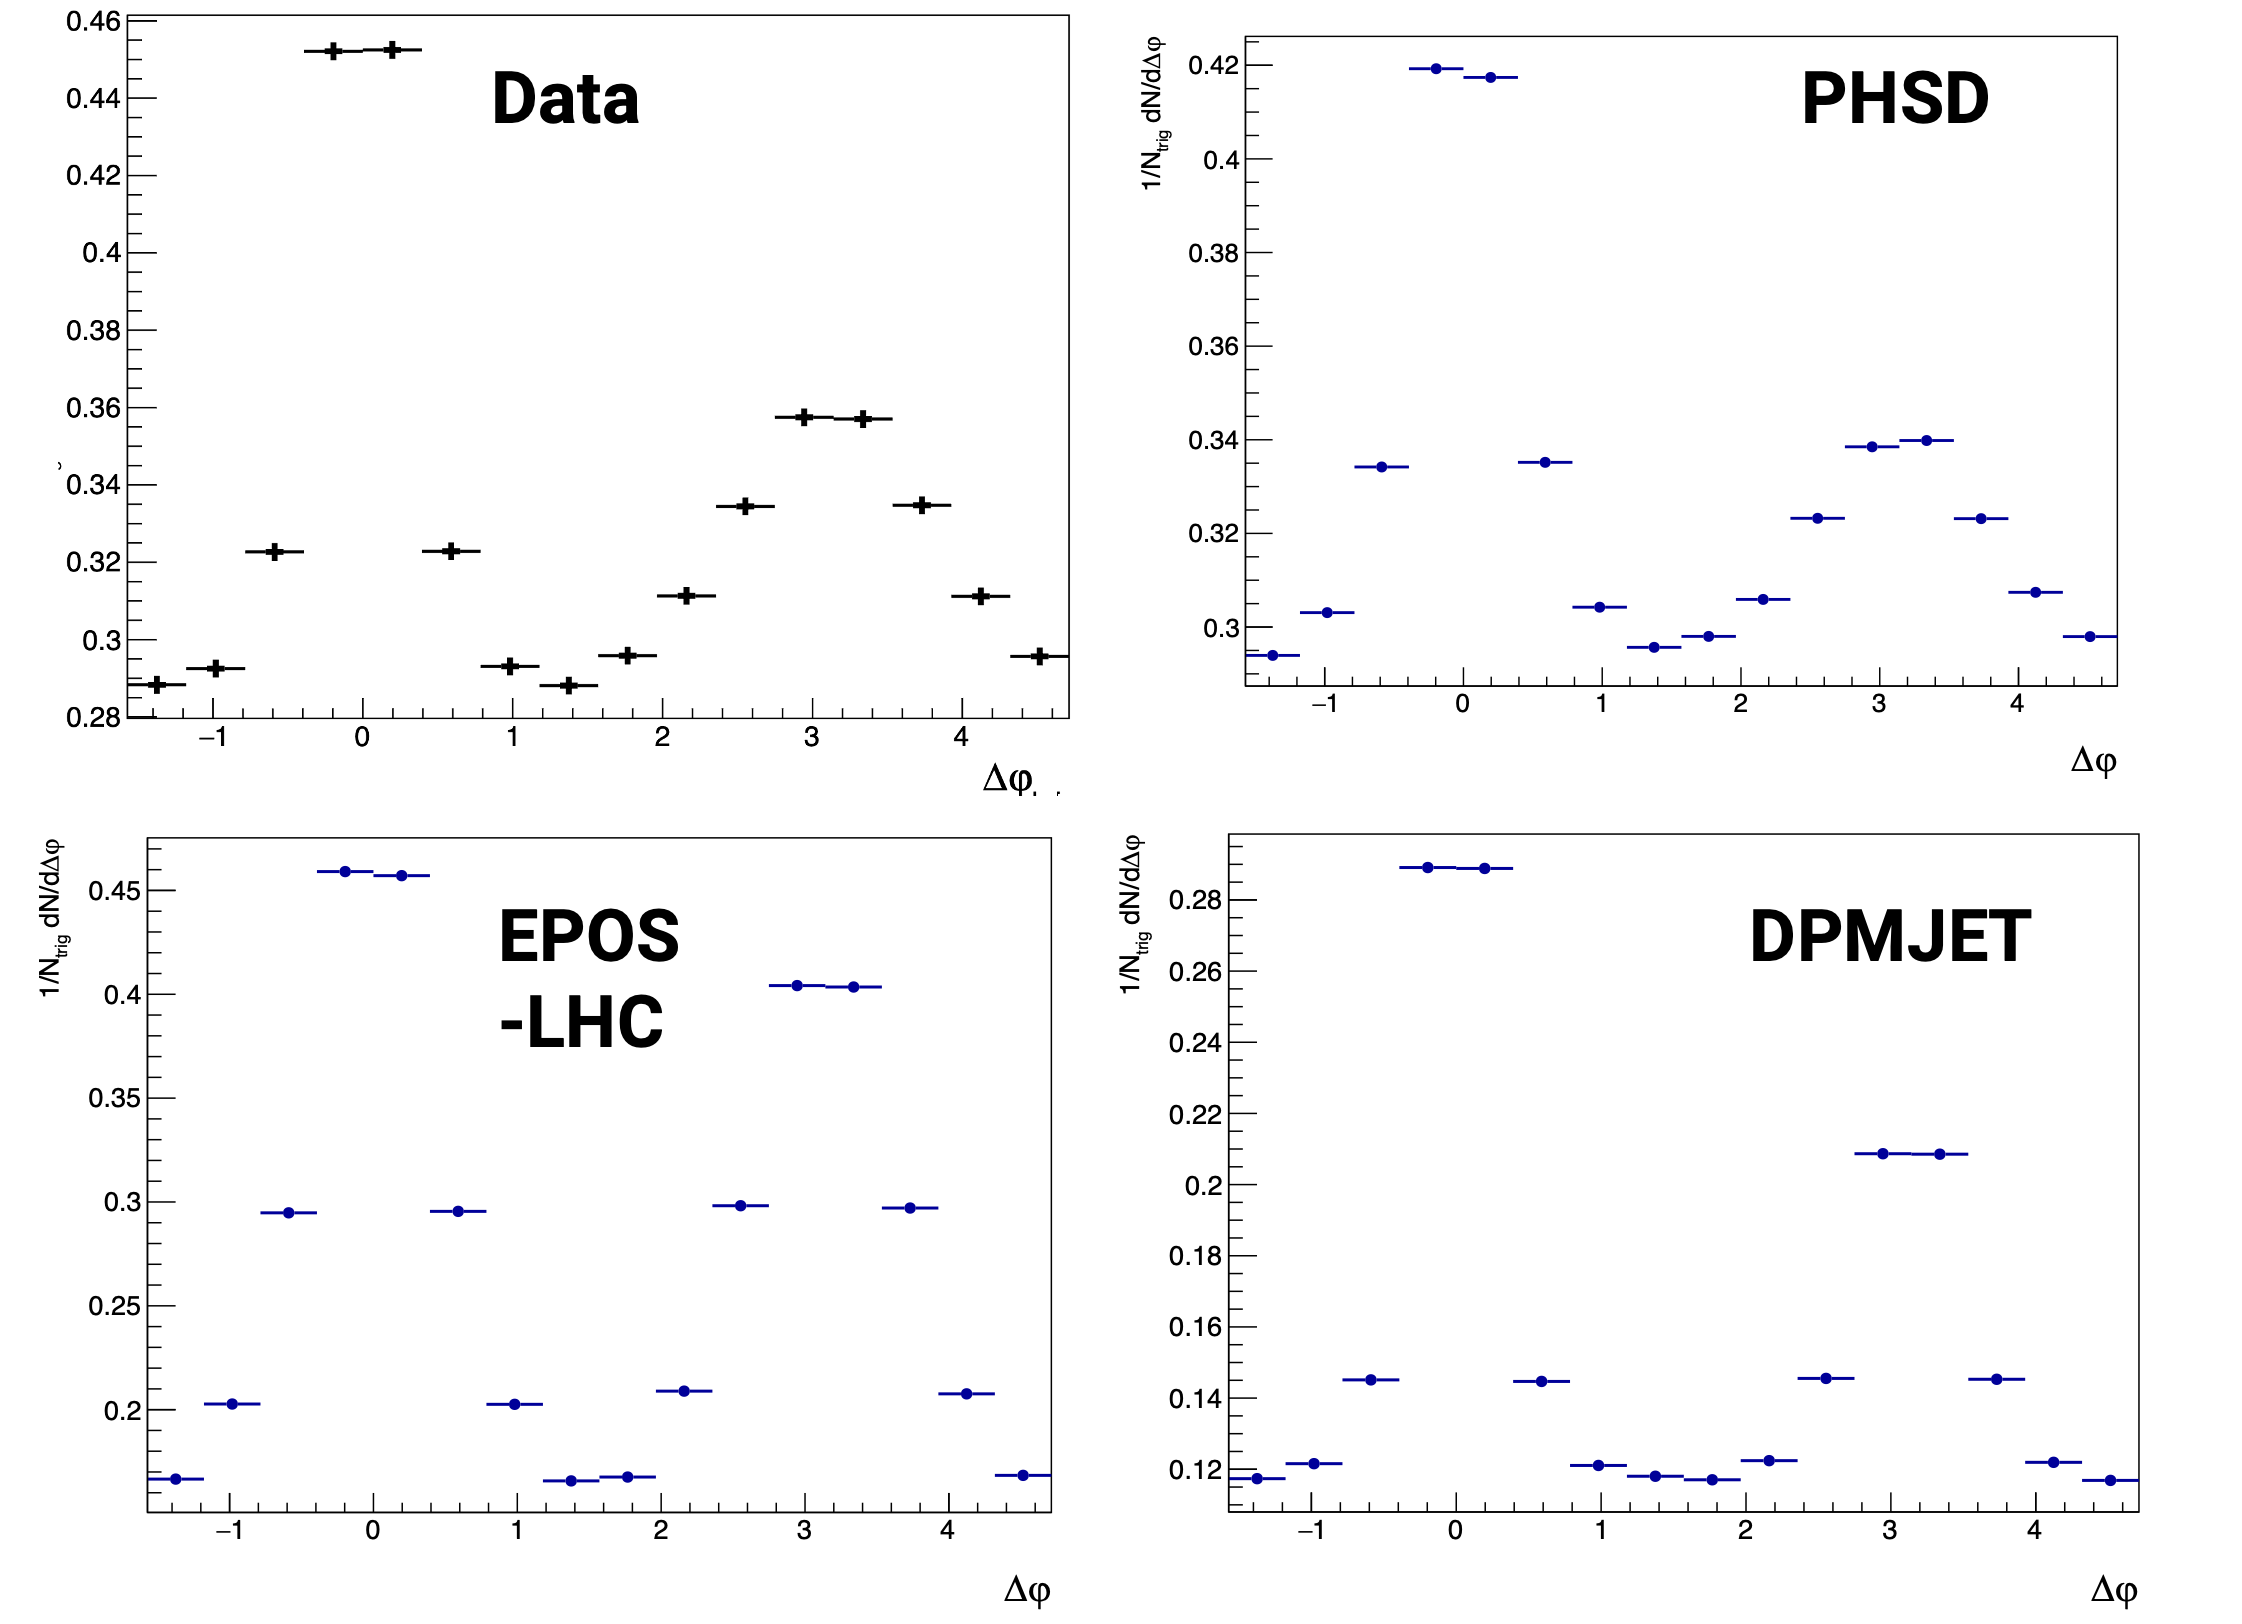
\includegraphics[width=3in]{figures/h_h_1d_modelcomp.png}}
\end{subfigure}
\caption{The multiplicity-integrated per-trigger $h-\Lambda$ (left) and $h-h$ (right) 1D $\Delta\eta\Delta\varphi$ distributions in data and for each model within our central associated $p_{T}$ bin (2.0 - 4.0 GeV/c).}
\label{1d_modelcomp}
\end{figure}

Due to difficulties with statistics (PHSD) and constraining the underlying event contribution (EPOS-LHC and PHSD), we will only be considering DPMJet for the following sections.

\subsubsection{Generating Multiplicity Percentiles}
\label{model_mult_percentiles}
As our final results are multiplicity-dependent, we must first sort our model-generated events into similar multiplicity percentiles as in data. To do this, we simply count the number of charged hadrons within the acceptance of our V0A detector (2.8 $< \eta <$ 5.1) for each event and use the corresponding distribution to generate the percentiles. The resulting distribution for each model can be seen in Figure \ref{model_mult_percentiles_figure}.

\begin{figure}[ht]
\centering
\begin{subfigure}{
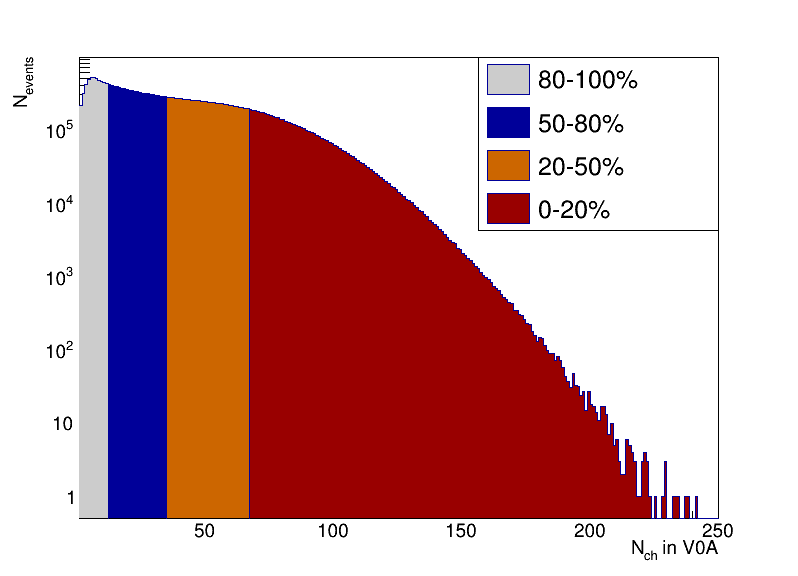
\includegraphics[width=3in]{figures/dpmjet_mult_dist.png}}
\end{subfigure}
\begin{subfigure}{
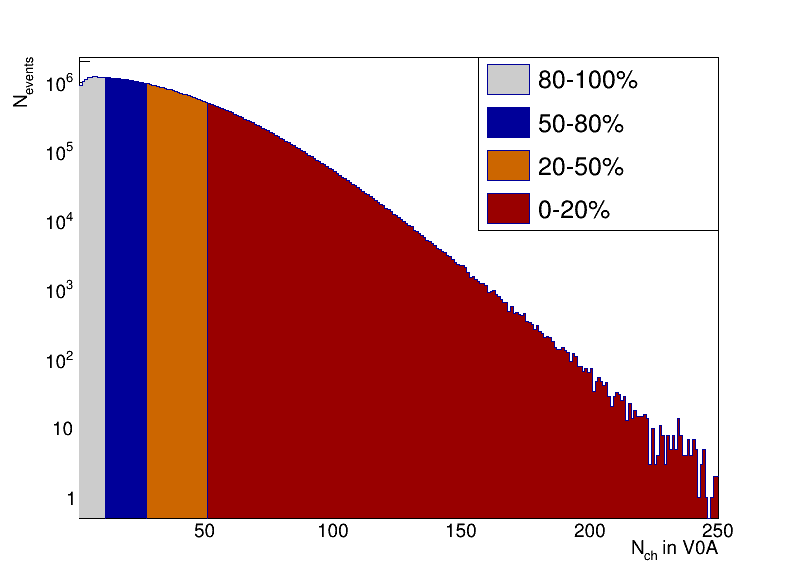
\includegraphics[width=3in]{figures/phsd_mult_dist.png}}
\end{subfigure}
\caption{The number of charged hadrons within the acceptance of our V0A detector (2.8 $< \eta <$ 5.1) in each event for DPMJet (left) and PHSD (right). These distributions were used to generate the multiplicity percentiles, which are colored in the figure.}
\label{model_mult_percentiles_figure}
\end{figure}

With the events sorted into multiplicity percentiles, we can now compare our final analysis results to the model(s). As mentioned previously, we will just be focusing on DPMJet for now.

\subsubsection{Systematic Uncertainties for DPMJet}
\label{dpmjet_systematics}
While most of the systematics considered for this analysis are not relevant for model predictions, both the yield extraction procedure and width extraction procedure have systematics that should be taken into account. We provide a table of the systematic uncertainties in each multiplicity bin for our central momentum bin for DPMJet in Tables \ref{dpmjet_systematics_table_lambda} ($h-\Lambda$) and \ref{dpmjet_systematics_table_h} ($h-h$).

\begin{table}[ht]
\centering
\begin{tabular}{|c||c|c|c|c|c|c|c|}
\hline
Mult. Bin & NS width & AS width & NS yield & AS yield & UE yield  & Total yield \\
\hline
0-20\% &  1.0 & 0.9 & 0.6 & 0.9 & 0.8 & 0.0 \\
20-50\% &  1.0 & 1.6 & 0.7 & 0.8 & 0.9 & 0.0 \\
50-80\% &  0.4 & 1.0 & 0.6 & 0.8 & 0.6 & 0.0 \\
\hline
\end{tabular}
\caption{The total systematic uncertainties associated with various extraction procedures in DPMJet for the $h-\Lambda$ distributions.}
\label{dpmjet_systematics_table_lambda}
\end{table}

\begin{table}[ht]
\centering
\begin{tabular}{|c||c|c|c|c|c|c|c|}
\hline
Mult. Bin & NS width & AS width & NS yield & AS yield & UE yield  & Total yield \\
\hline
0-20\% &  0.9 & 1.2 & 1.0 & 0.7 & 0.9 & 0.0 \\
20-50\% &  0.7 & 1.2 & 1.0 & 0.7 & 0.7 & 0.0 \\
50-80\% &  0.3 & 1.3 & 0.6 & 0.7 & 0.6 & 0.0 \\
\hline
\end{tabular}
\caption{The total systematic uncertainties associated with various extraction procedures in DPMJet for the $h-h$ distributions.}
\label{dpmjet_systematics_table_h}
\end{table}

\subsubsection{Multiplicity Dependent Per-trigger Jet-like Yields}
\label{pairwise_yields_modelcomp}
The per-trigger pairwise jet-like yields for both the $h-\Lambda$ and $h-h$ distributions  as a function of multiplicity for each associated $p_{T}$ bin in data and using DPMJet can be seen in Figure \ref{pairwise_yields_modelcomp_figure}.

We see that DPMJet does a fairly good job predicting the dihadron near- and away-side yields, but severely underestimates the $h-\Lambda$ yields. We also observe no multiplicity dependence for DPMJet in any of the distributions, which is in stark contrast to the $h-\Lambda$ data.

\begin{figure}[ht]
\centering
\begin{subfigure}{
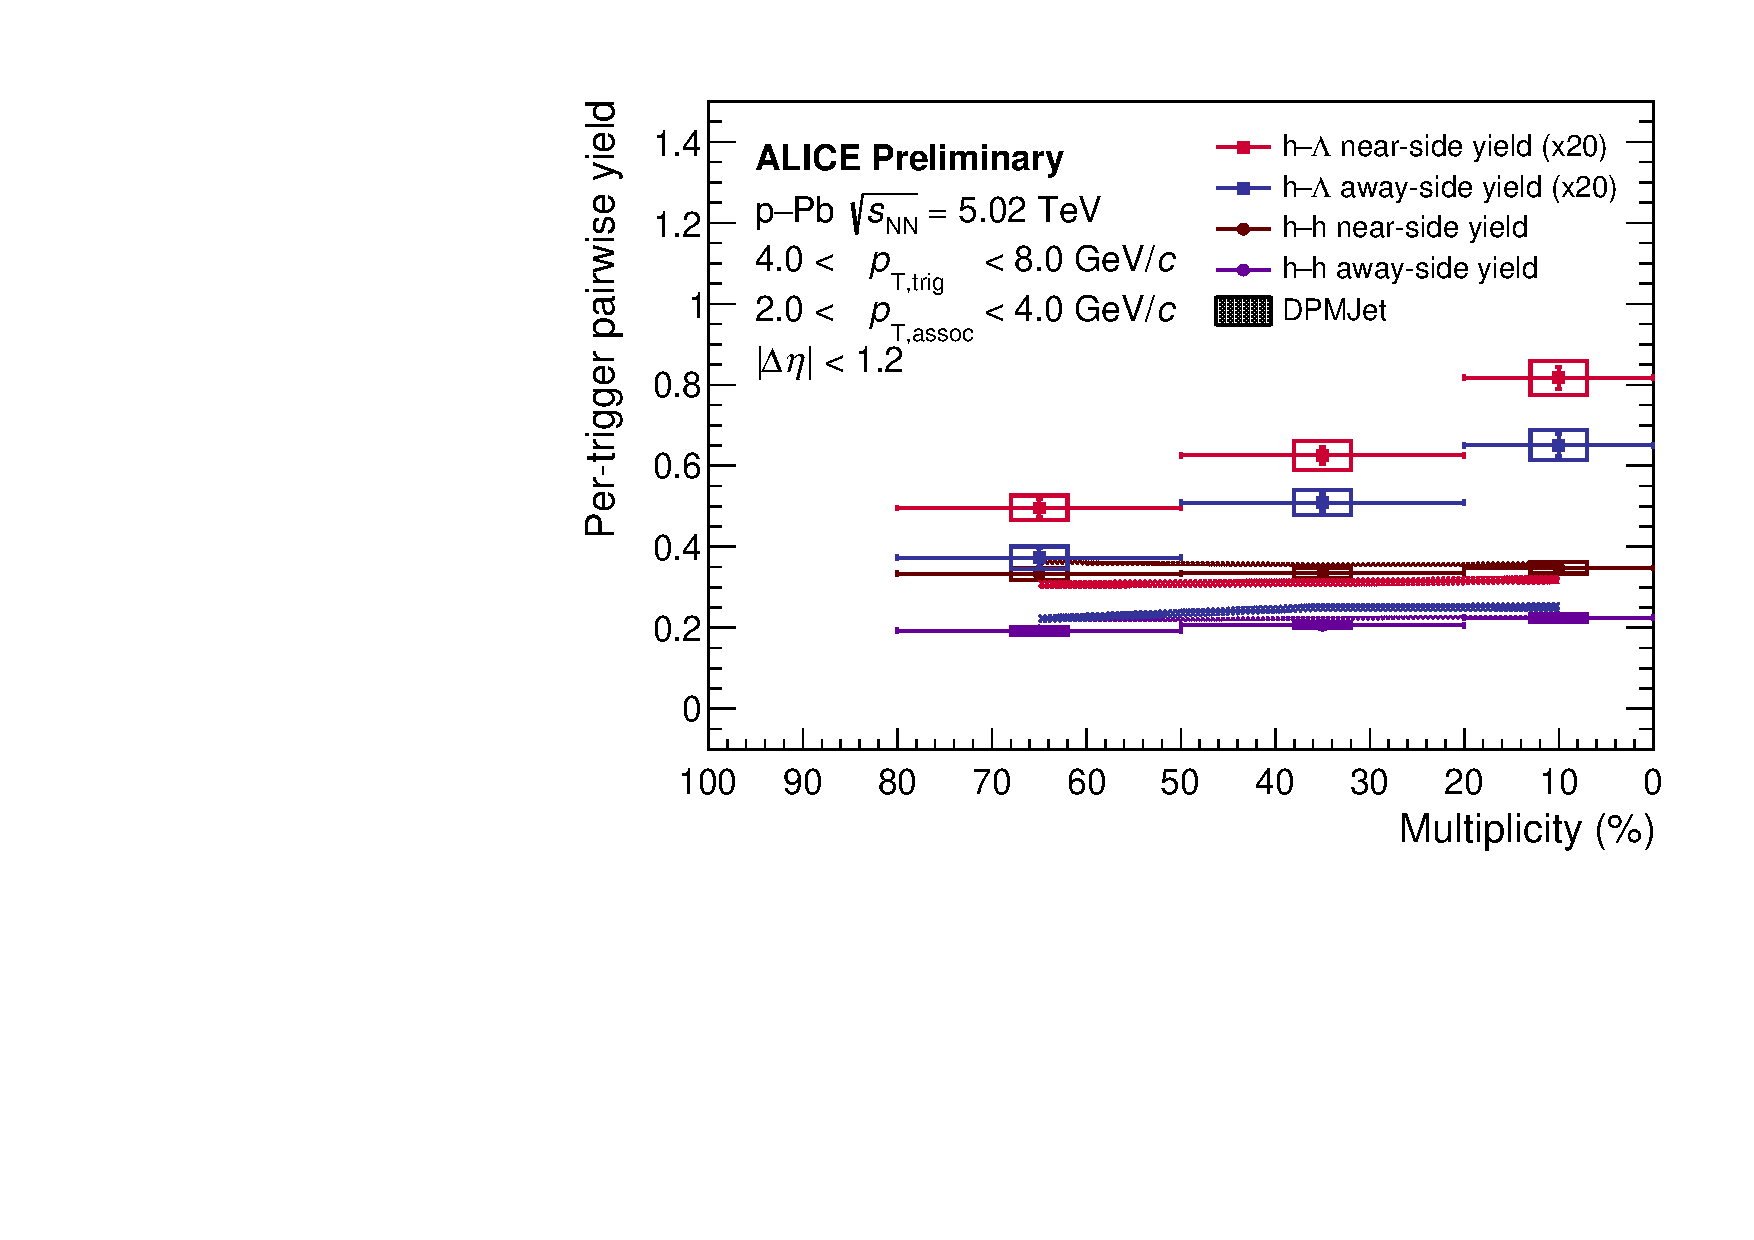
\includegraphics[width=4in]{figures/pairwise_plot_with_dpmjet.pdf}}
\end{subfigure}
\begin{subfigure}{
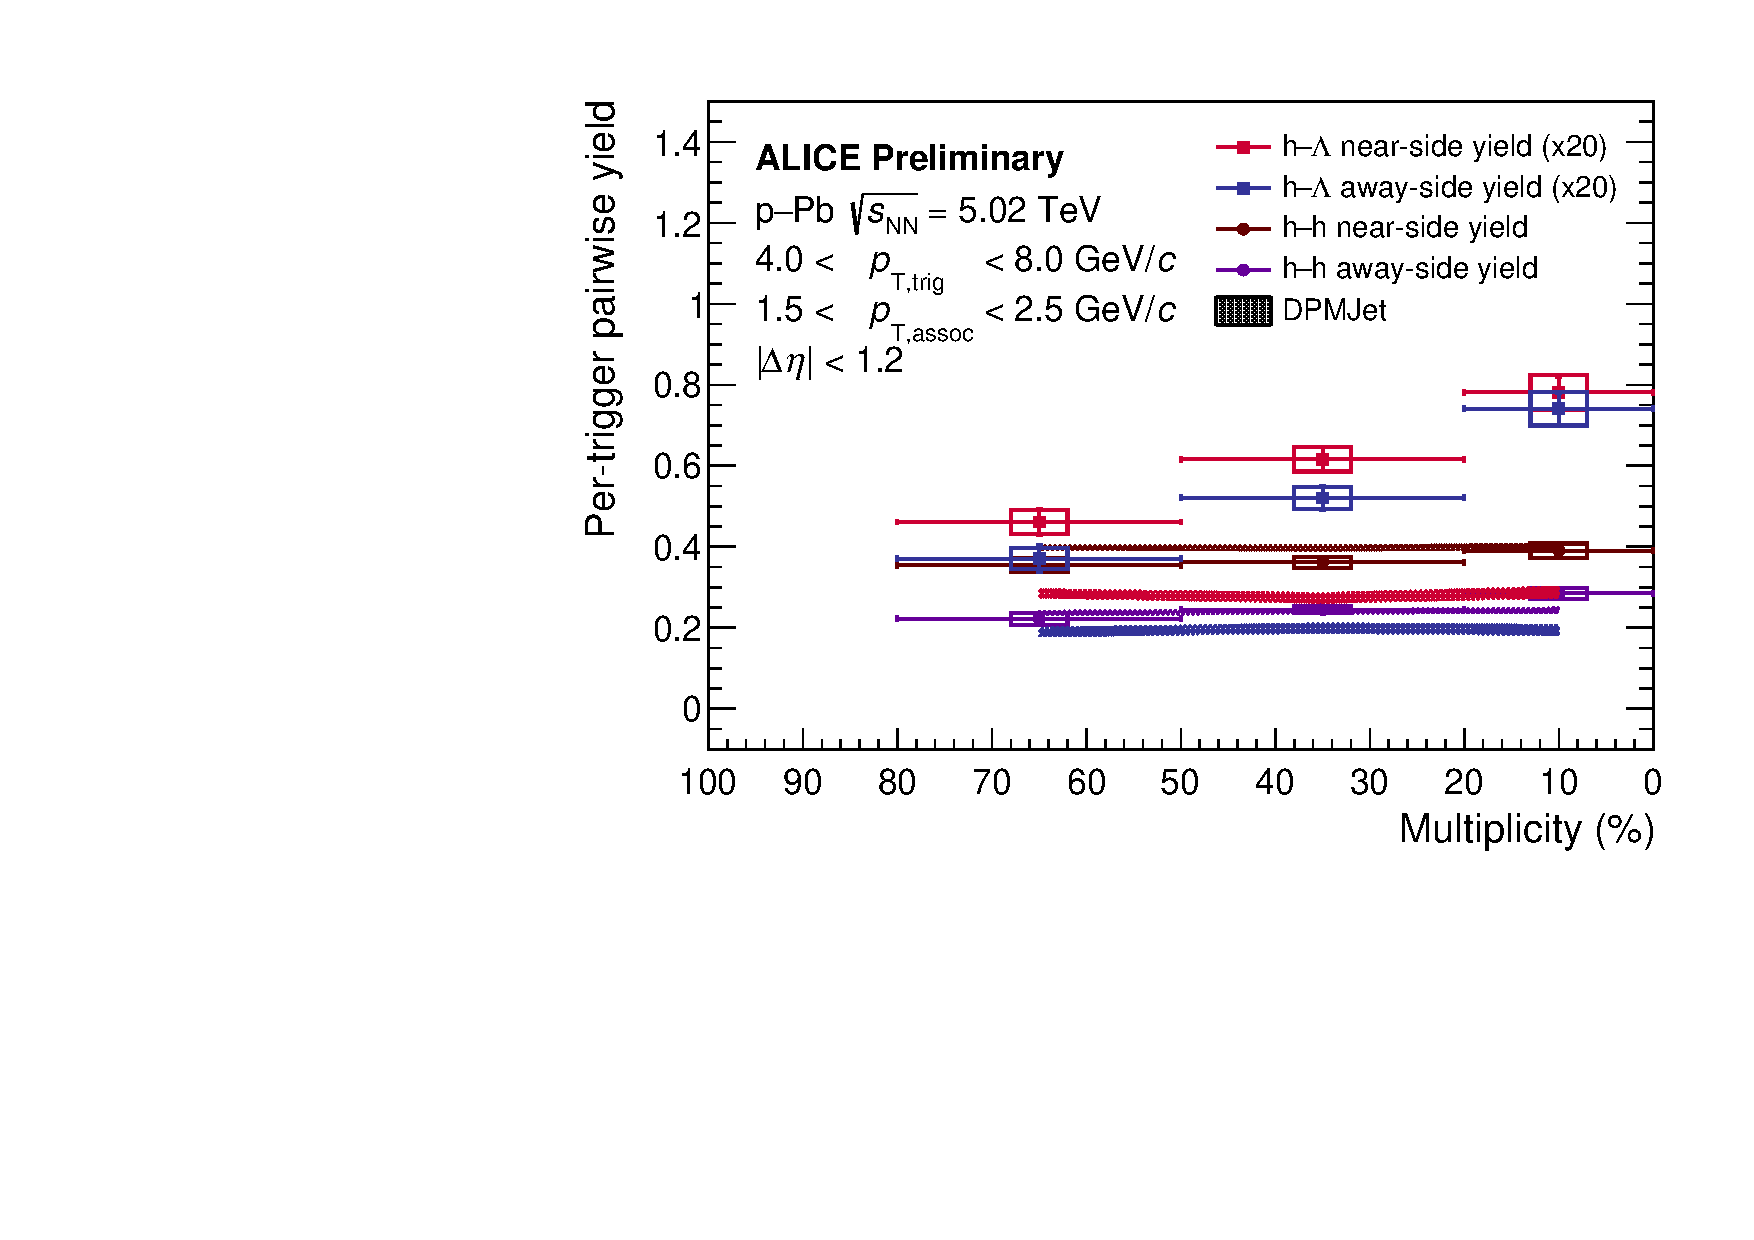
\includegraphics[width=4in]{figures/pairwise_plot_lowpt_with_dpmjet.pdf}}
\end{subfigure}
\begin{subfigure}{
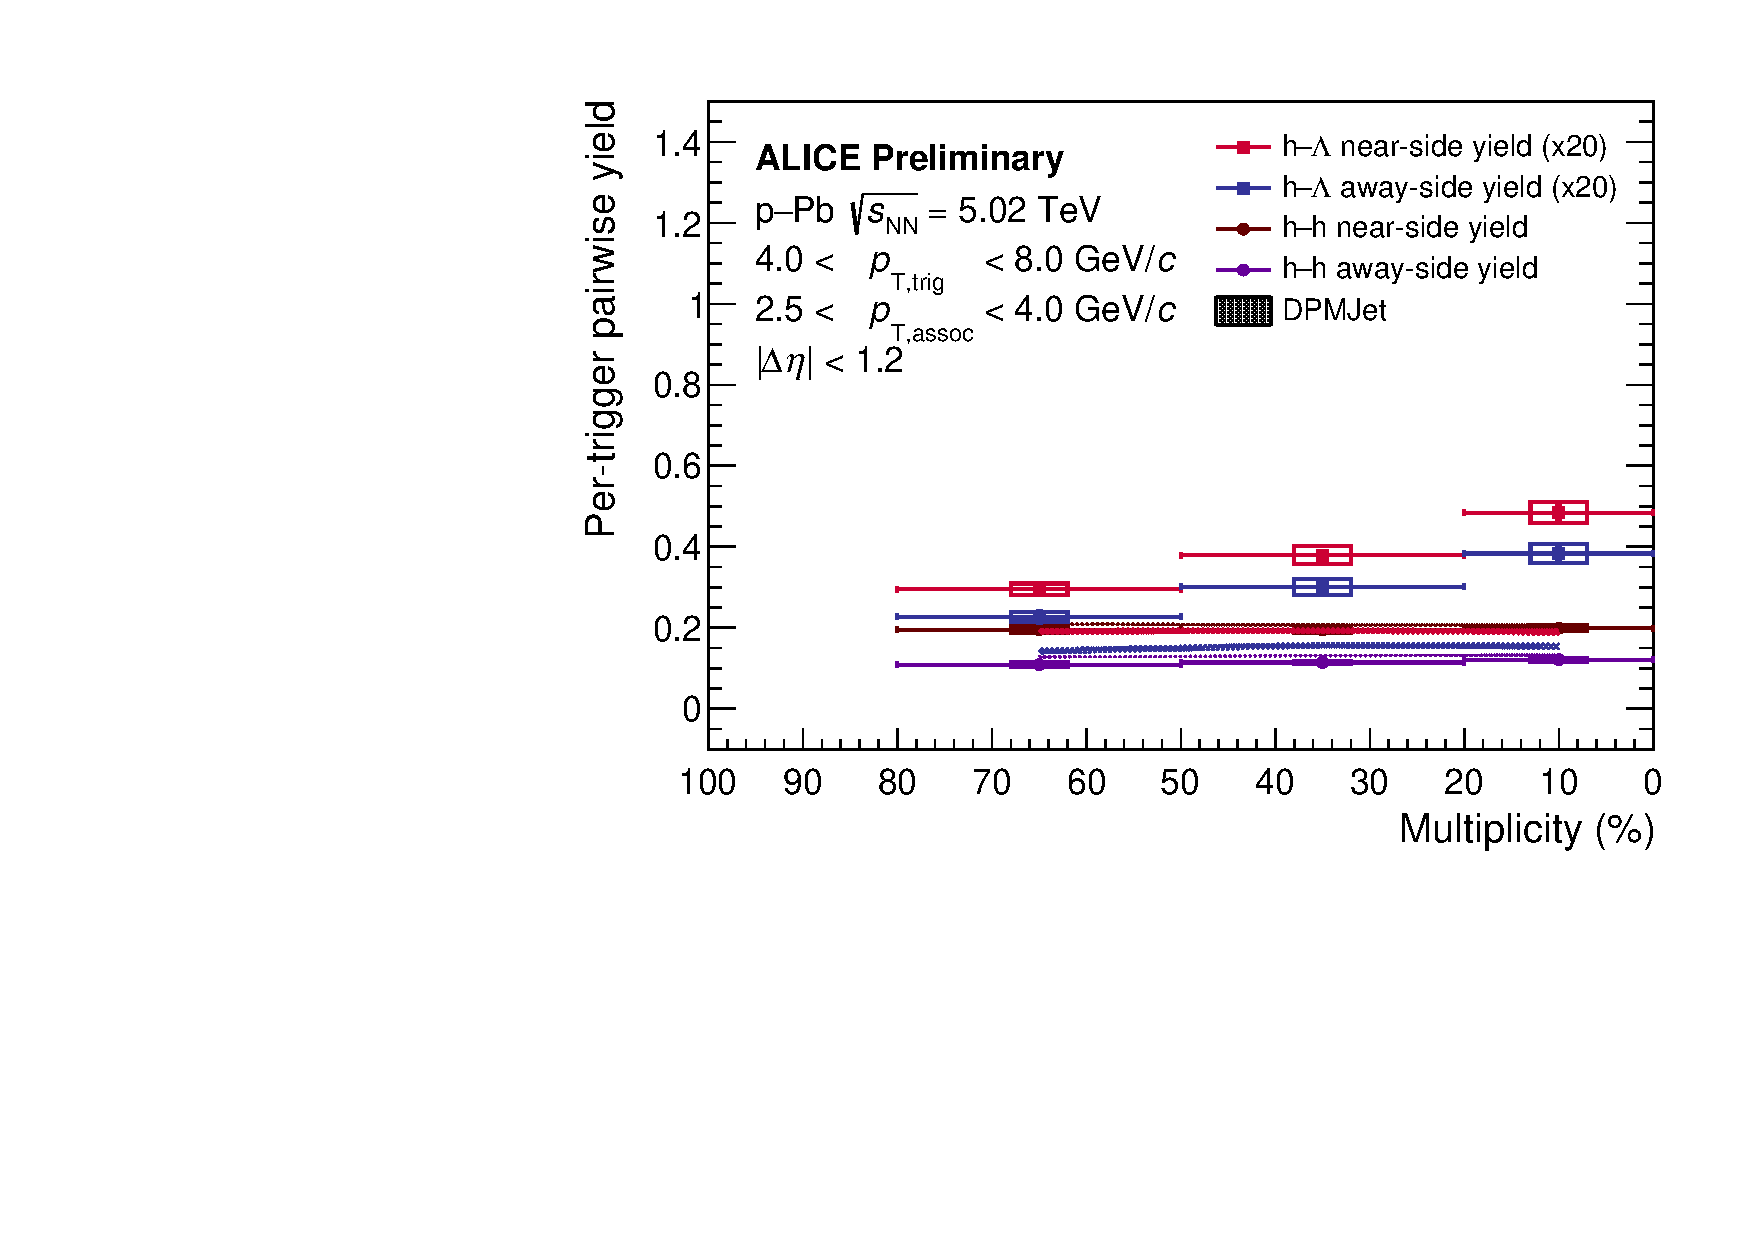
\includegraphics[width=4in]{figures/pairwise_plot_highpt_with_dpmjet.pdf}}
\end{subfigure}
\caption{The per-trigger pairwise jet-like yields of the $h-\Lambda$ and $h-h$ distributions as a function of multiplicity for each associated $p_{T}$ bin in data and using DPMJet. The top, middle and bottom plots correspond to the 2.0 - 4.0 GeV/c, 1.5 - 2.5 GeV/c and 2.5 - 4.0 GeV/c associated $p_{T}$ bins, respectively.}
\label{pairwise_yields_modelcomp_figure}
\end{figure}

\subsubsection{Multiplicity Dependent ($h-\Lambda$)/($h-h$) Ratios}
\label{lambda_hadron_ratio_modelcomp}

The ratio of per-trigger yields of $h-\Lambda$/$h-h$ pairs in each of the kinematic regions as a function of multiplicity for each associated $p_{T}$ bin in data and using DPMJet can be seen in Figure \ref{lambda_hadron_ratio_modelcomp_figure}. We have elected to exclude the total ratio, as it crowds the plot (and can be inferred by the other ratios). 

We see that DPMJet actually manages to preserve the relative ordering of the ratios in each kinematic region, with the underlying event on top, followed by the away-side jet and then the near-side jet. However, DPMJet underestimates the magnitude of the ratios in each kinematic region, and each ratio also shows little-to-no dependence on multiplicity. The jet-like ratios also appear to increase with increasing $p_{T}$, whereas the underlying event ratio appears constant.

\begin{figure}[ht]
\centering
\begin{subfigure}{
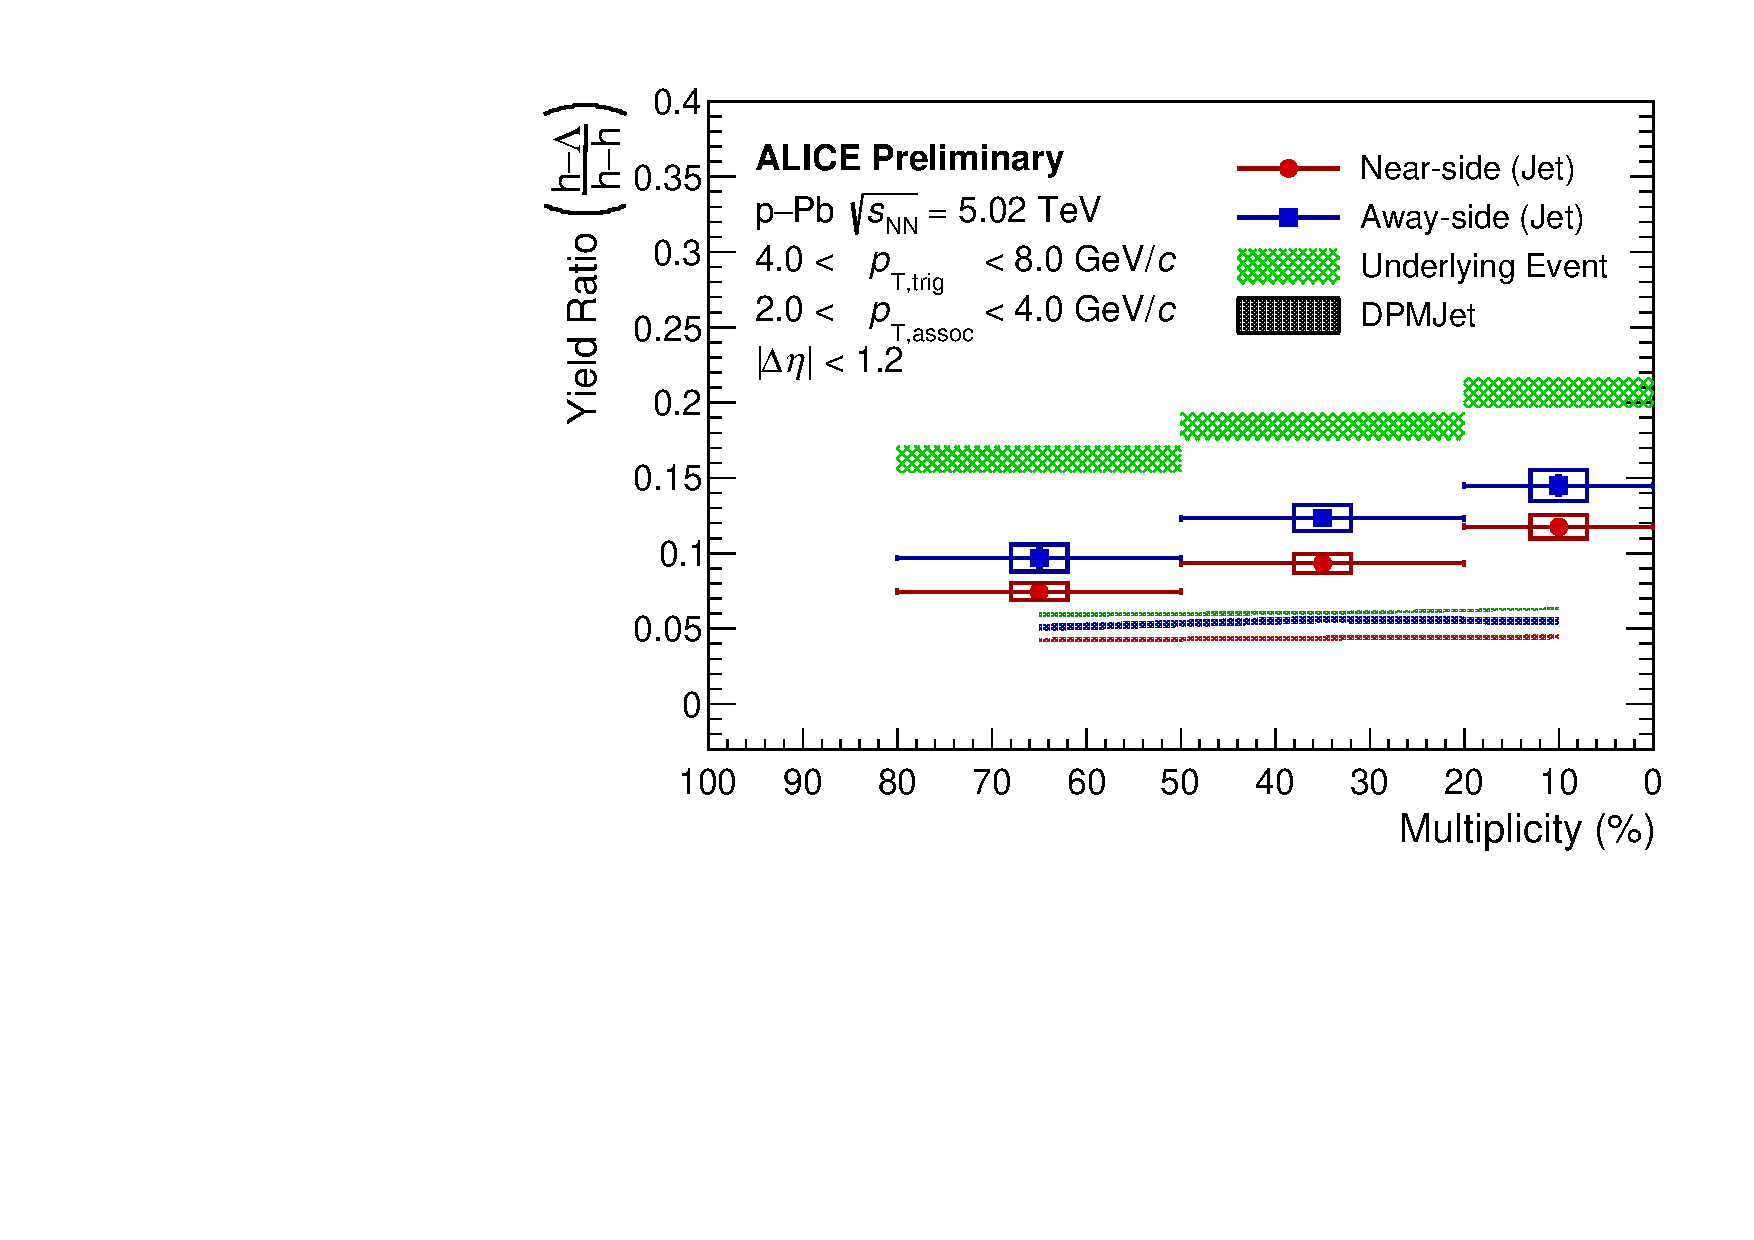
\includegraphics[width=4in]{figures/ratio_plot_with_dpmjet.pdf}}
\end{subfigure}
\begin{subfigure}{
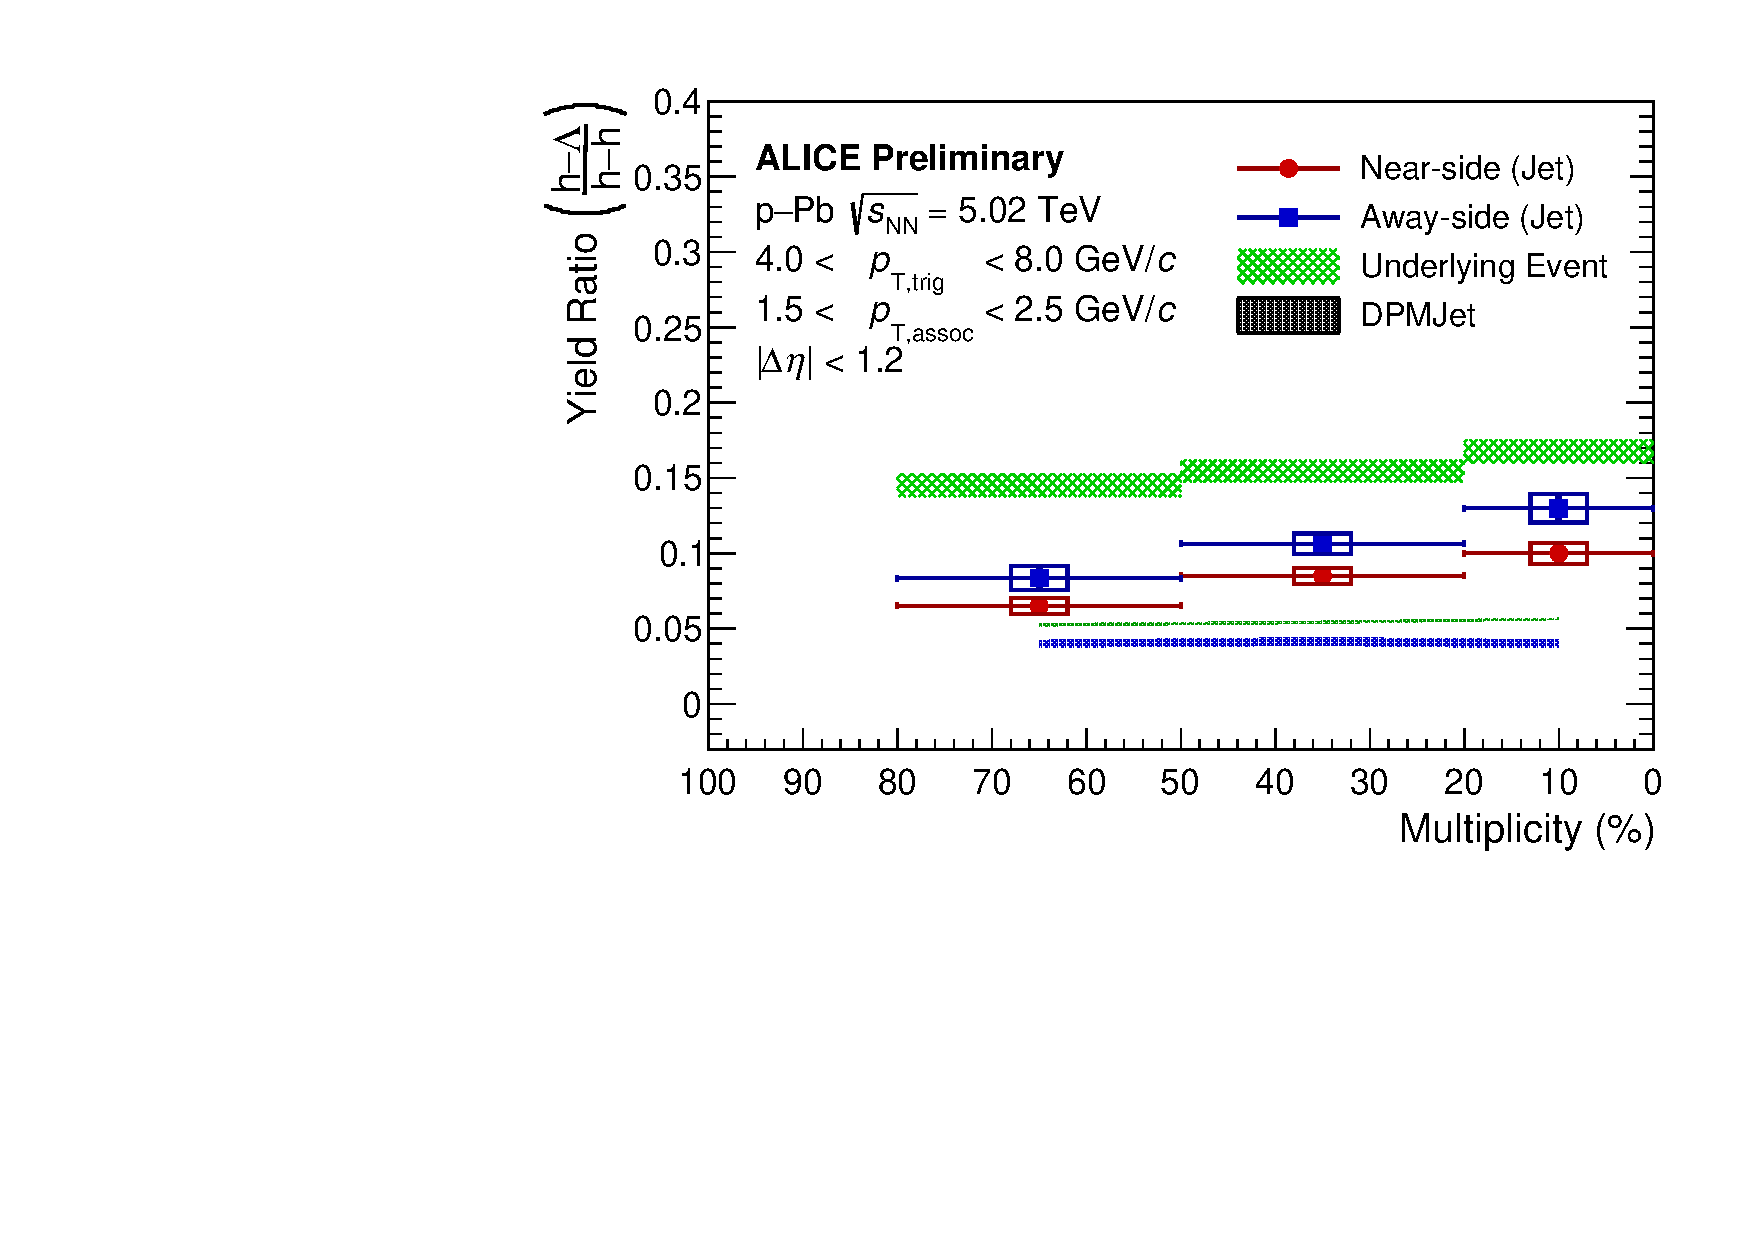
\includegraphics[width=4in]{figures/ratio_plot_lowpt_with_dpmjet.pdf}}
\end{subfigure}
\begin{subfigure}{
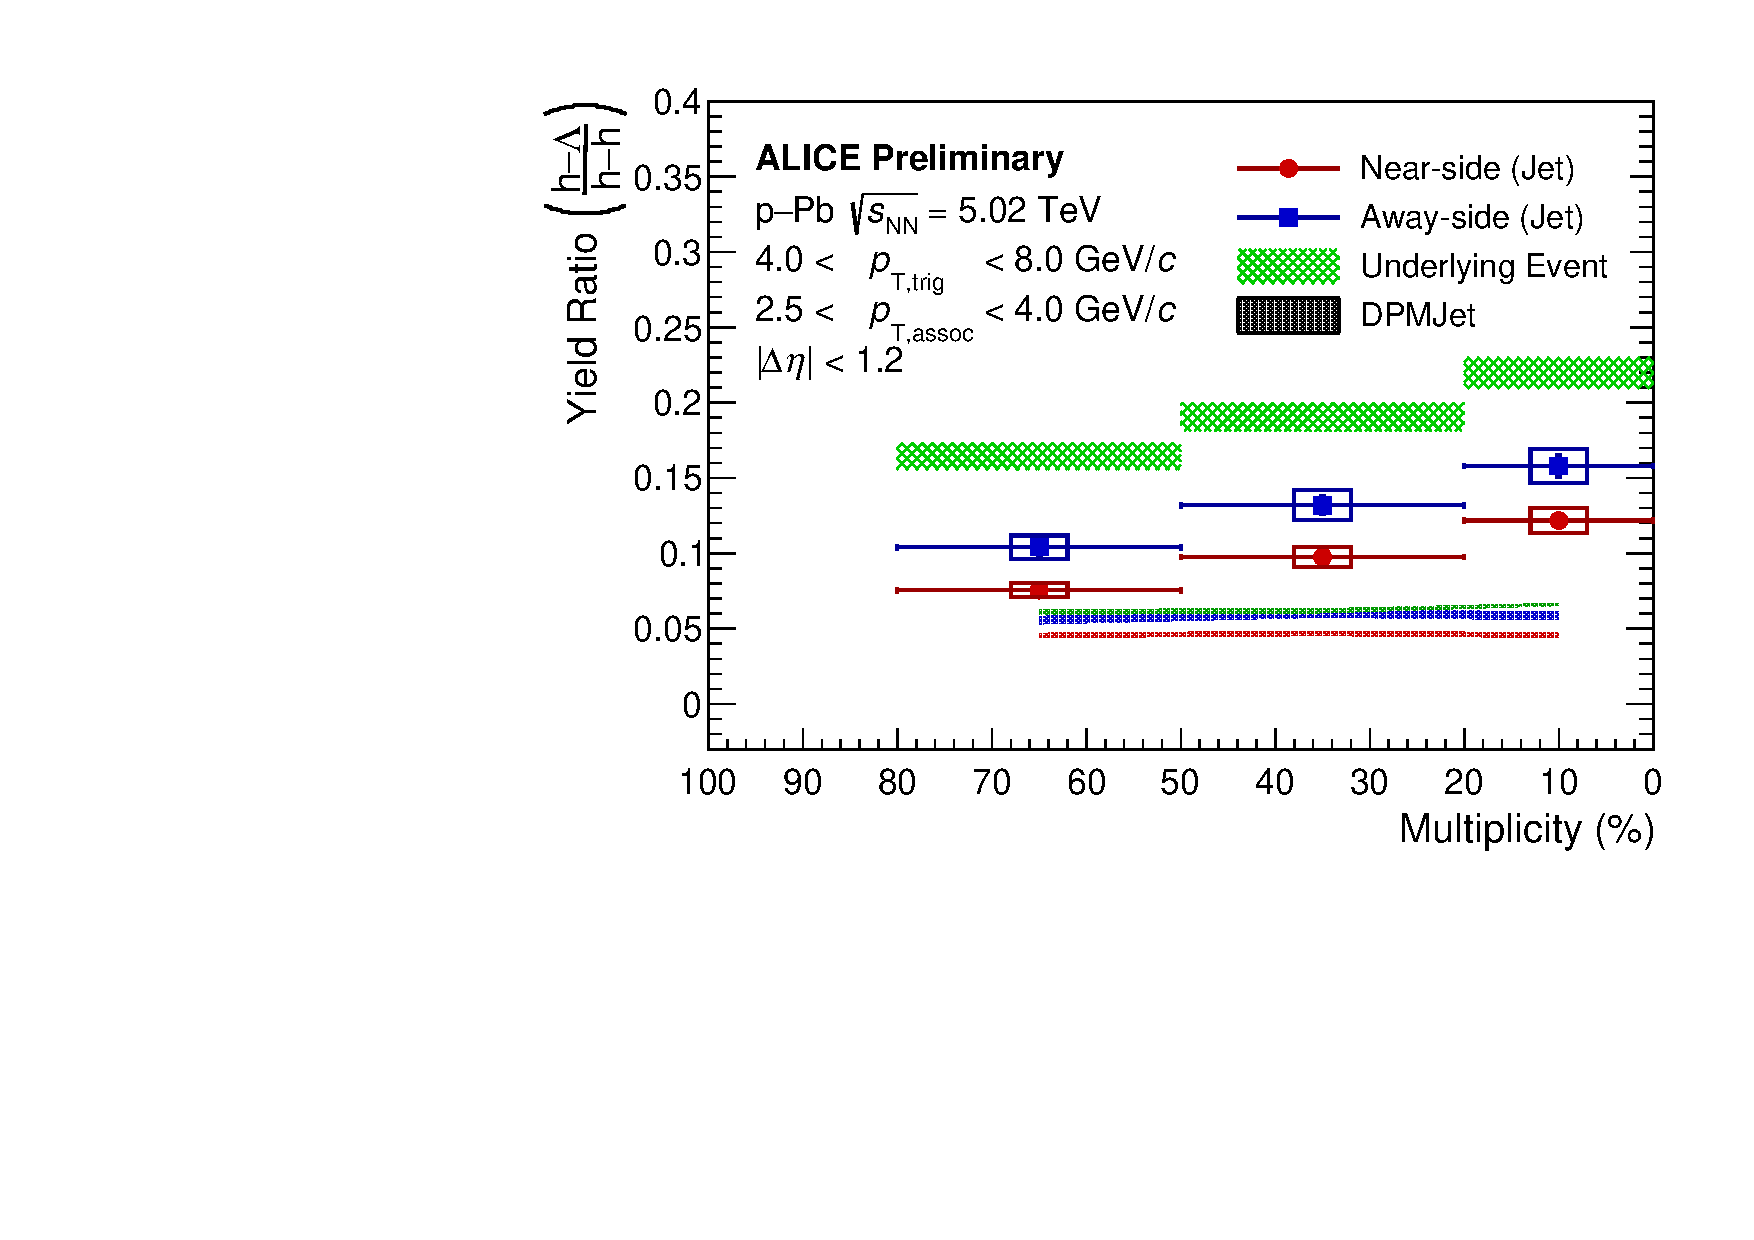
\includegraphics[width=4in]{figures/ratio_plot_highpt_with_dpmjet.pdf}}
\end{subfigure}
\caption{The ratio of per-trigger yields of $h-\Lambda$/$h-h$ pairs in each of the kinematic regions as a function of multiplicity for each associated $p_{T}$ bin in data and using DPMJet. The top, middle and bottom plots correspond to the 2.0 - 4.0 GeV/c, 1.5 - 2.5 GeV/c and 2.5 - 4.0 GeV/c associated $p_{T}$ bins, respectively.}
\label{lambda_hadron_ratio_modelcomp_figure}
\end{figure}


\subsubsection{Multiplicity Dependent ($h-\Lambda$)/($h-\phi$) Ratios}
\label{lambda_phi_ratio_modelcomp}

The ratio of per-trigger yields of $h-\Lambda$/$h-\phi$ pairs in each of the kinematic regions as a function of multiplicity for each associated $p_{T}$ bin in data and using DPMJet can be seen in Figure \ref{lambda_phi_ratio_modelcomp_figure}. We have elected to exclude the total ratio, as it crowds the plot (and can be inferred by the other ratios). 

Like data, DPMJet shows a clear separation between the underlying event and the jet-like ratios. However, DPMJet underestimates the magnitude of the ratios in each kinematic region. Furthermore, DPMJet also shows little-to-no difference between the near-side and away-side ratios. DPMJet also exhibits very little multiplicity or $p_{T}$ dependence for the ratios in each region.

\begin{figure}[ht]
\centering
\begin{subfigure}{
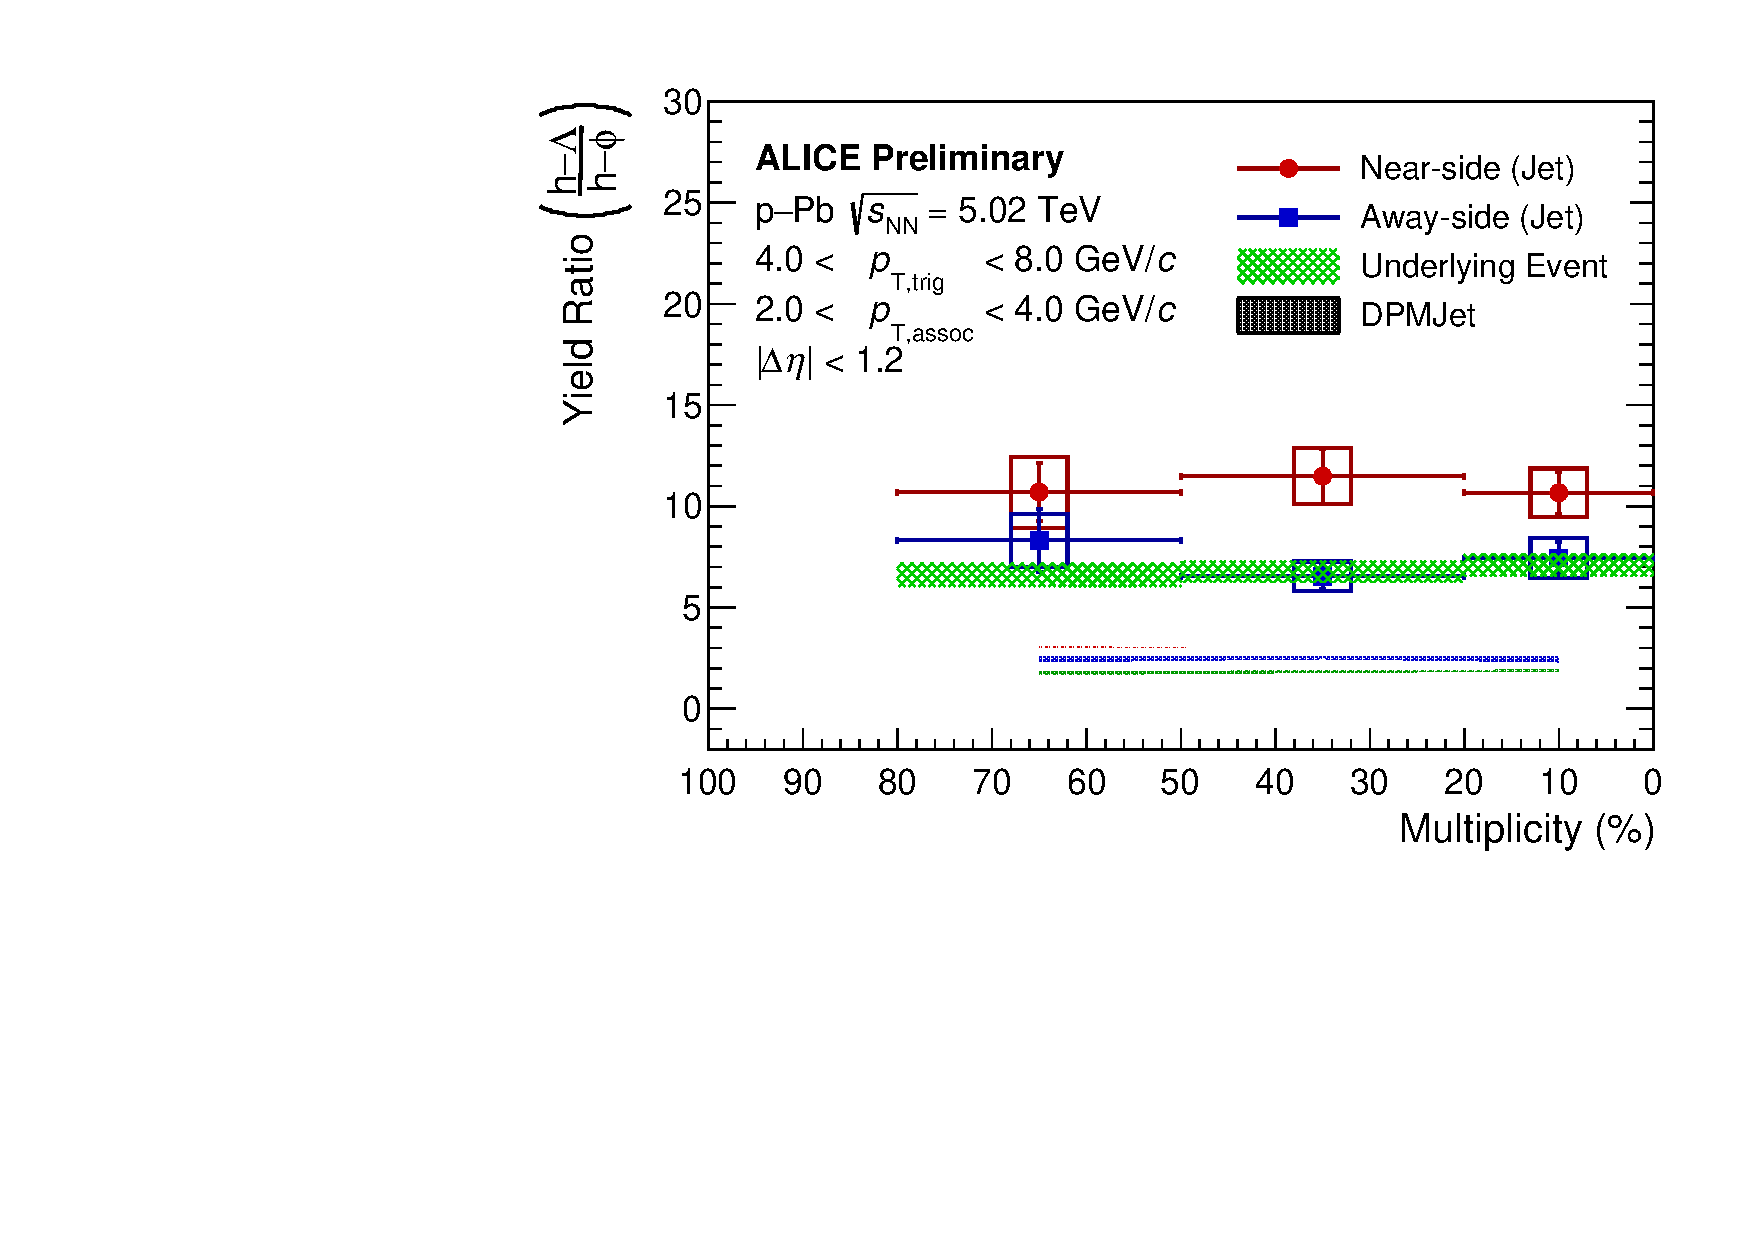
\includegraphics[width=4in]{figures/lambda_phi_ratio_plot_with_dpmjet.pdf}}
\end{subfigure}
\begin{subfigure}{
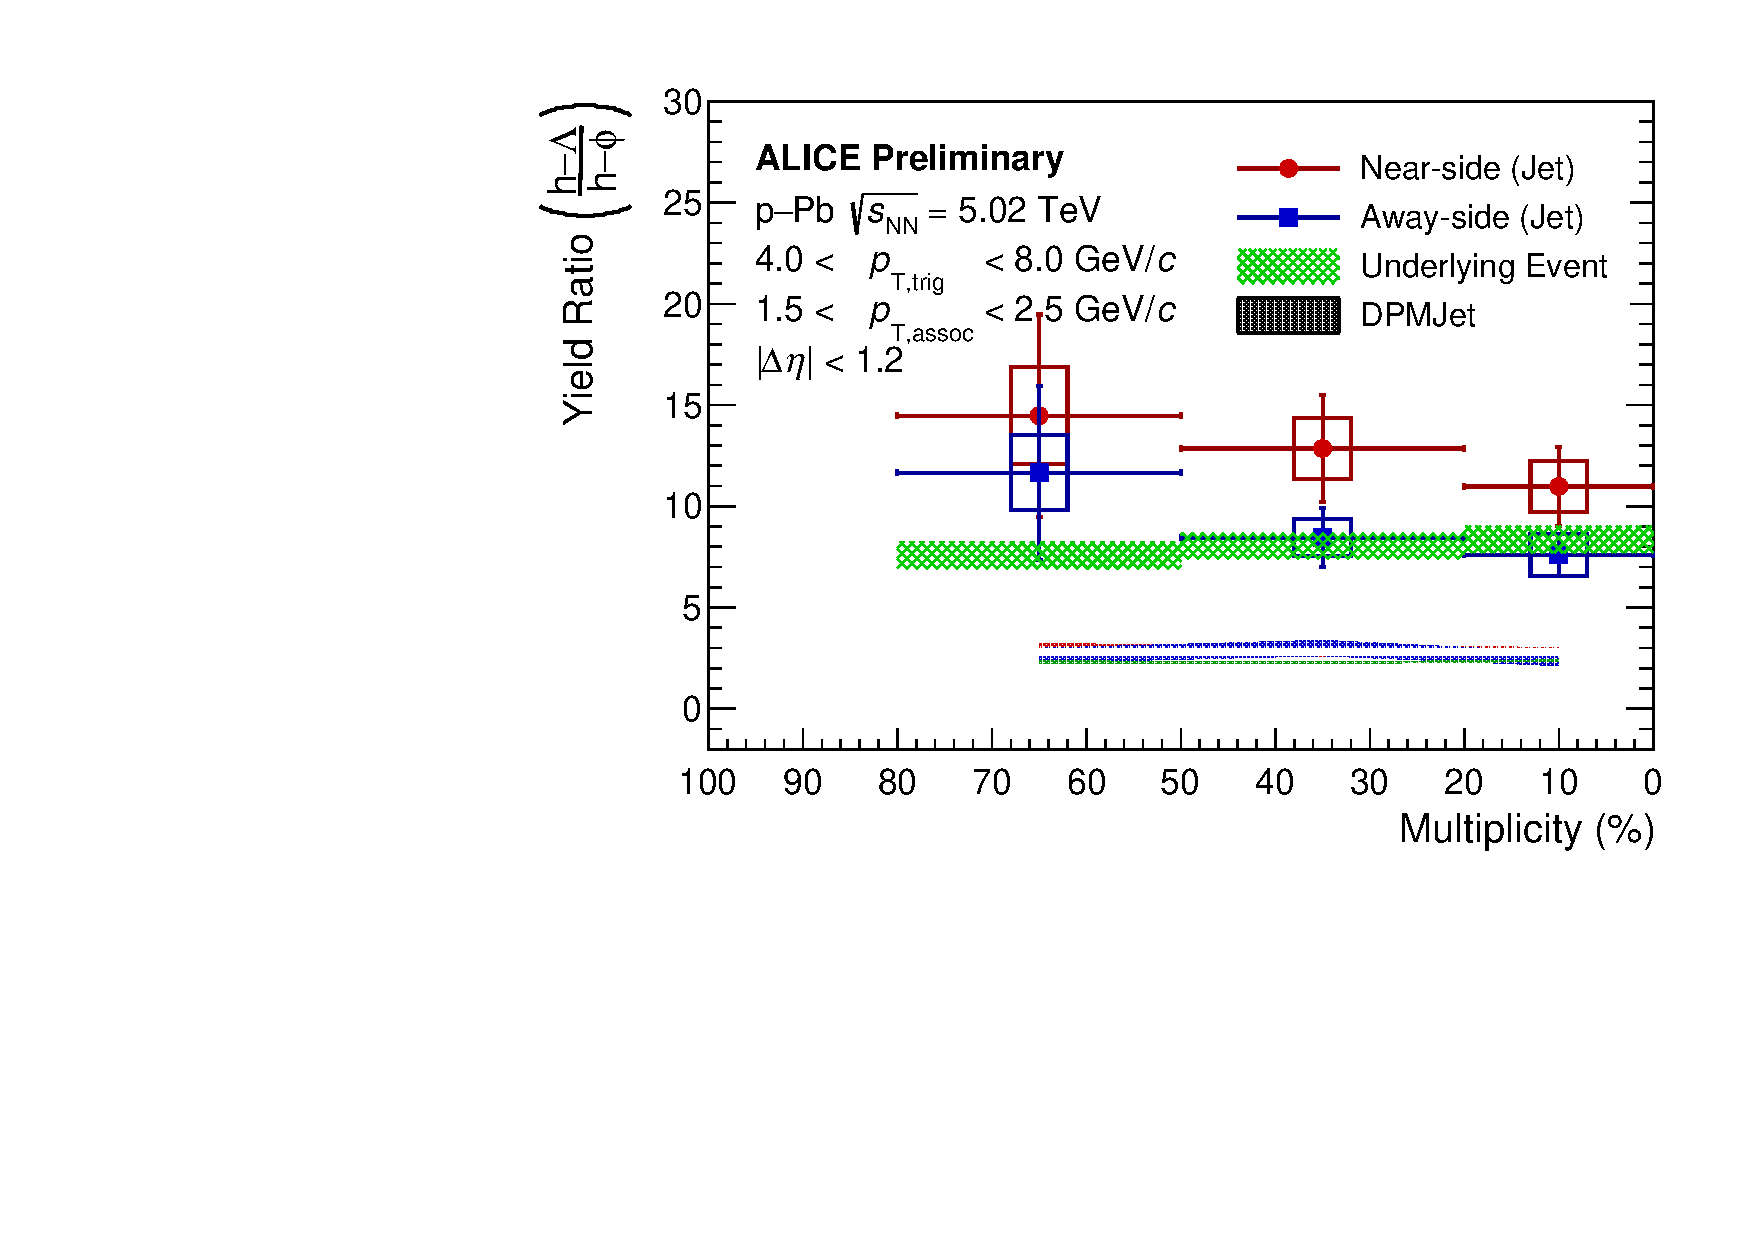
\includegraphics[width=4in]{figures/lambda_phi_ratio_plot_lowpt_with_dpmjet.pdf}}
\end{subfigure}
\begin{subfigure}{
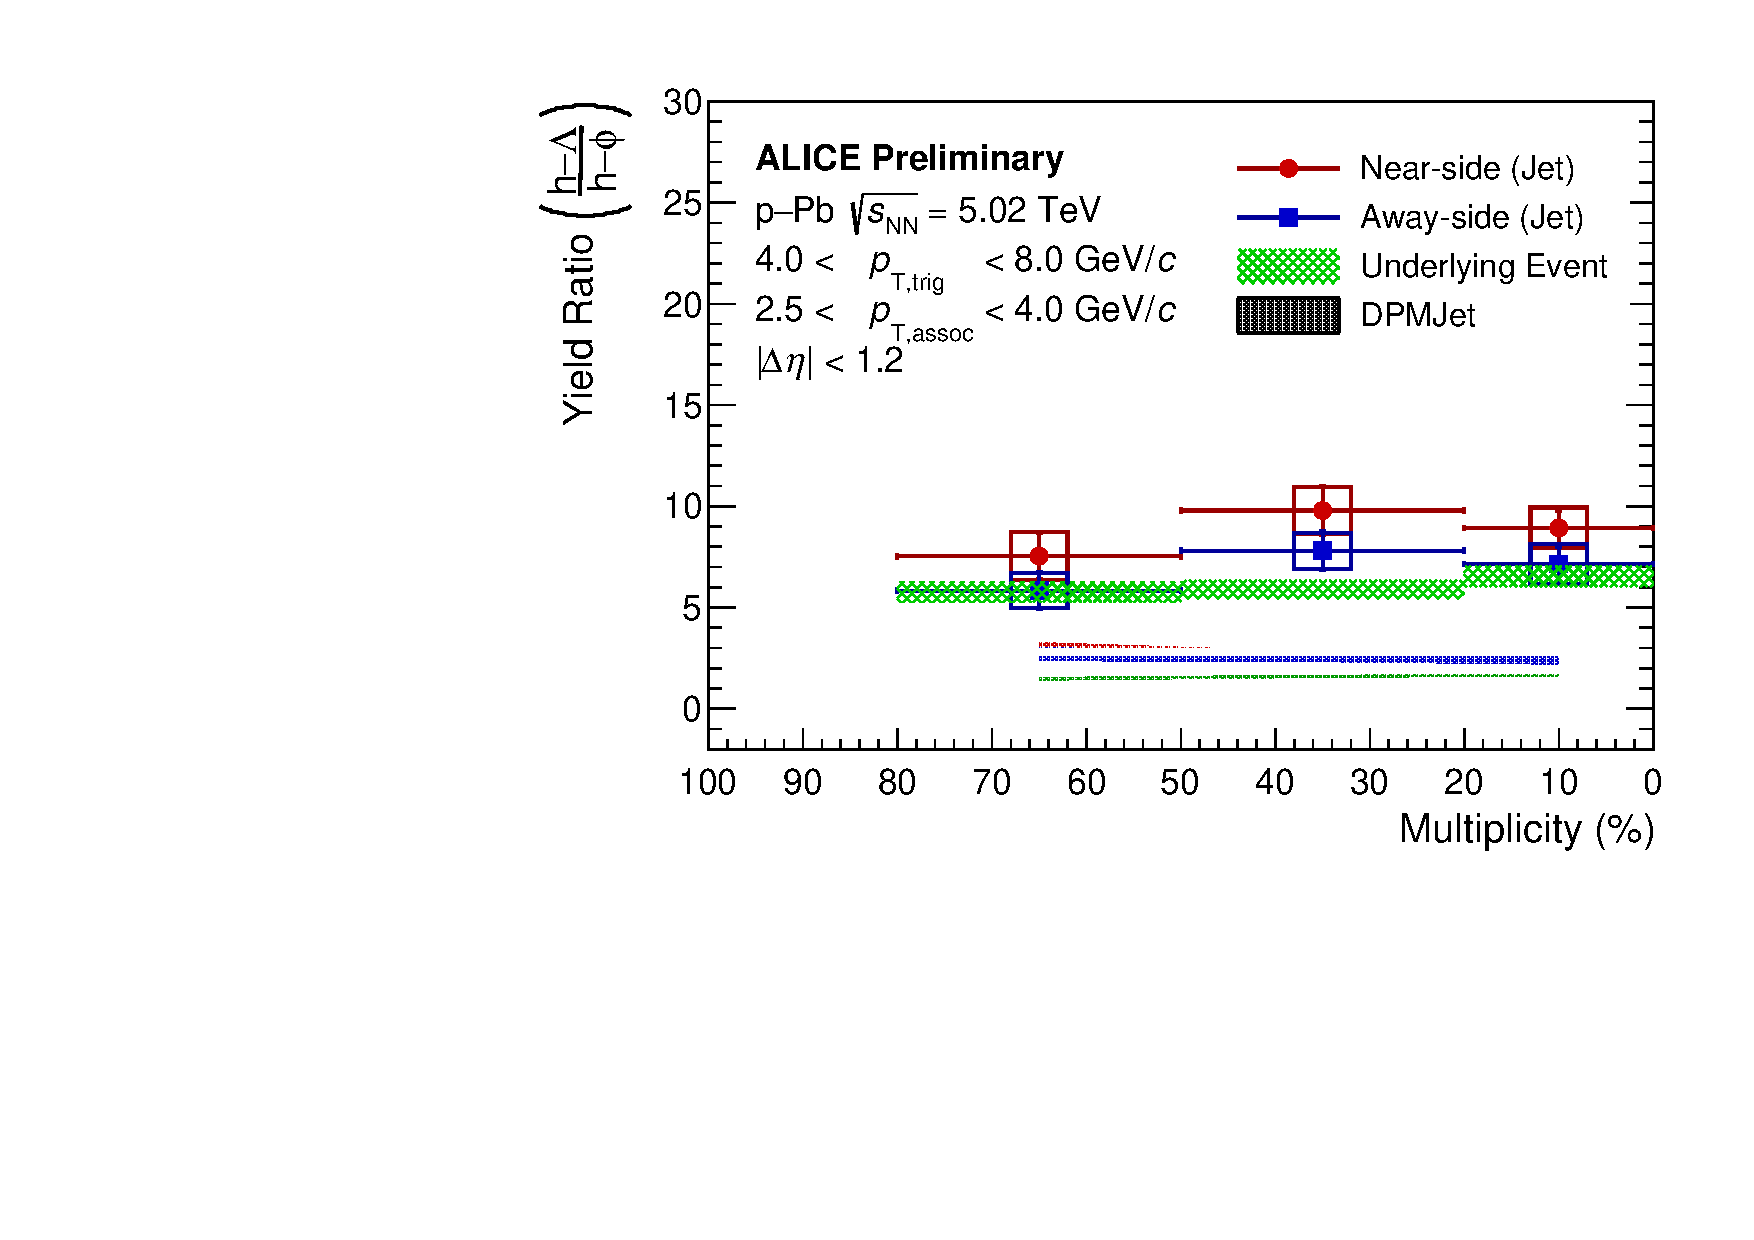
\includegraphics[width=4in]{figures/lambda_phi_ratio_plot_highpt_with_dpmjet.pdf}}
\end{subfigure}
\caption{The ratio of per-trigger yields of $h-\Lambda$/$h-h$ pairs in each of the kinematic regions as a function of multiplicity for each associated $p_{T}$ bin in data and using DPMJet. The top, middle and bottom plots correspond to the 2.0 - 4.0 GeV/c, 1.5 - 2.5 GeV/c and 2.5 - 4.0 GeV/c associated $p_{T}$ bins, respectively.}
\label{lambda_phi_ratio_modelcomp_figure}
\end{figure}

\subsubsection{Multiplicity Dependent Near- and Away-Side Widths}
\label{width_modelcomp}
The extracted near- and away-side widths of both the $h-\Lambda$ and $h-h$ distributions as a function of multiplicity for each associated $p_{T}$ bin in data and using DPMJet can be seen in Figure \ref{width_modelcomp_figure}. 

We see that DPMJet is mostly able to reproduce the near-side widths of the $h-h$ distributions for each associated $p_{T}$ bin, but underestimates the near-side widths of the $h-\Lambda$ distributions. DPMJet also underestimates the away-side widths of both the $h-h$ and $h-\Lambda$ distributions for each associated $p_{T}$ and multiplicity bin. There is also no observable multiplicity dependence for either the near- or away-side widths in DPMJet for every associated $p_{T}$ bin.

\begin{figure}[ht]
\centering
\begin{subfigure}{
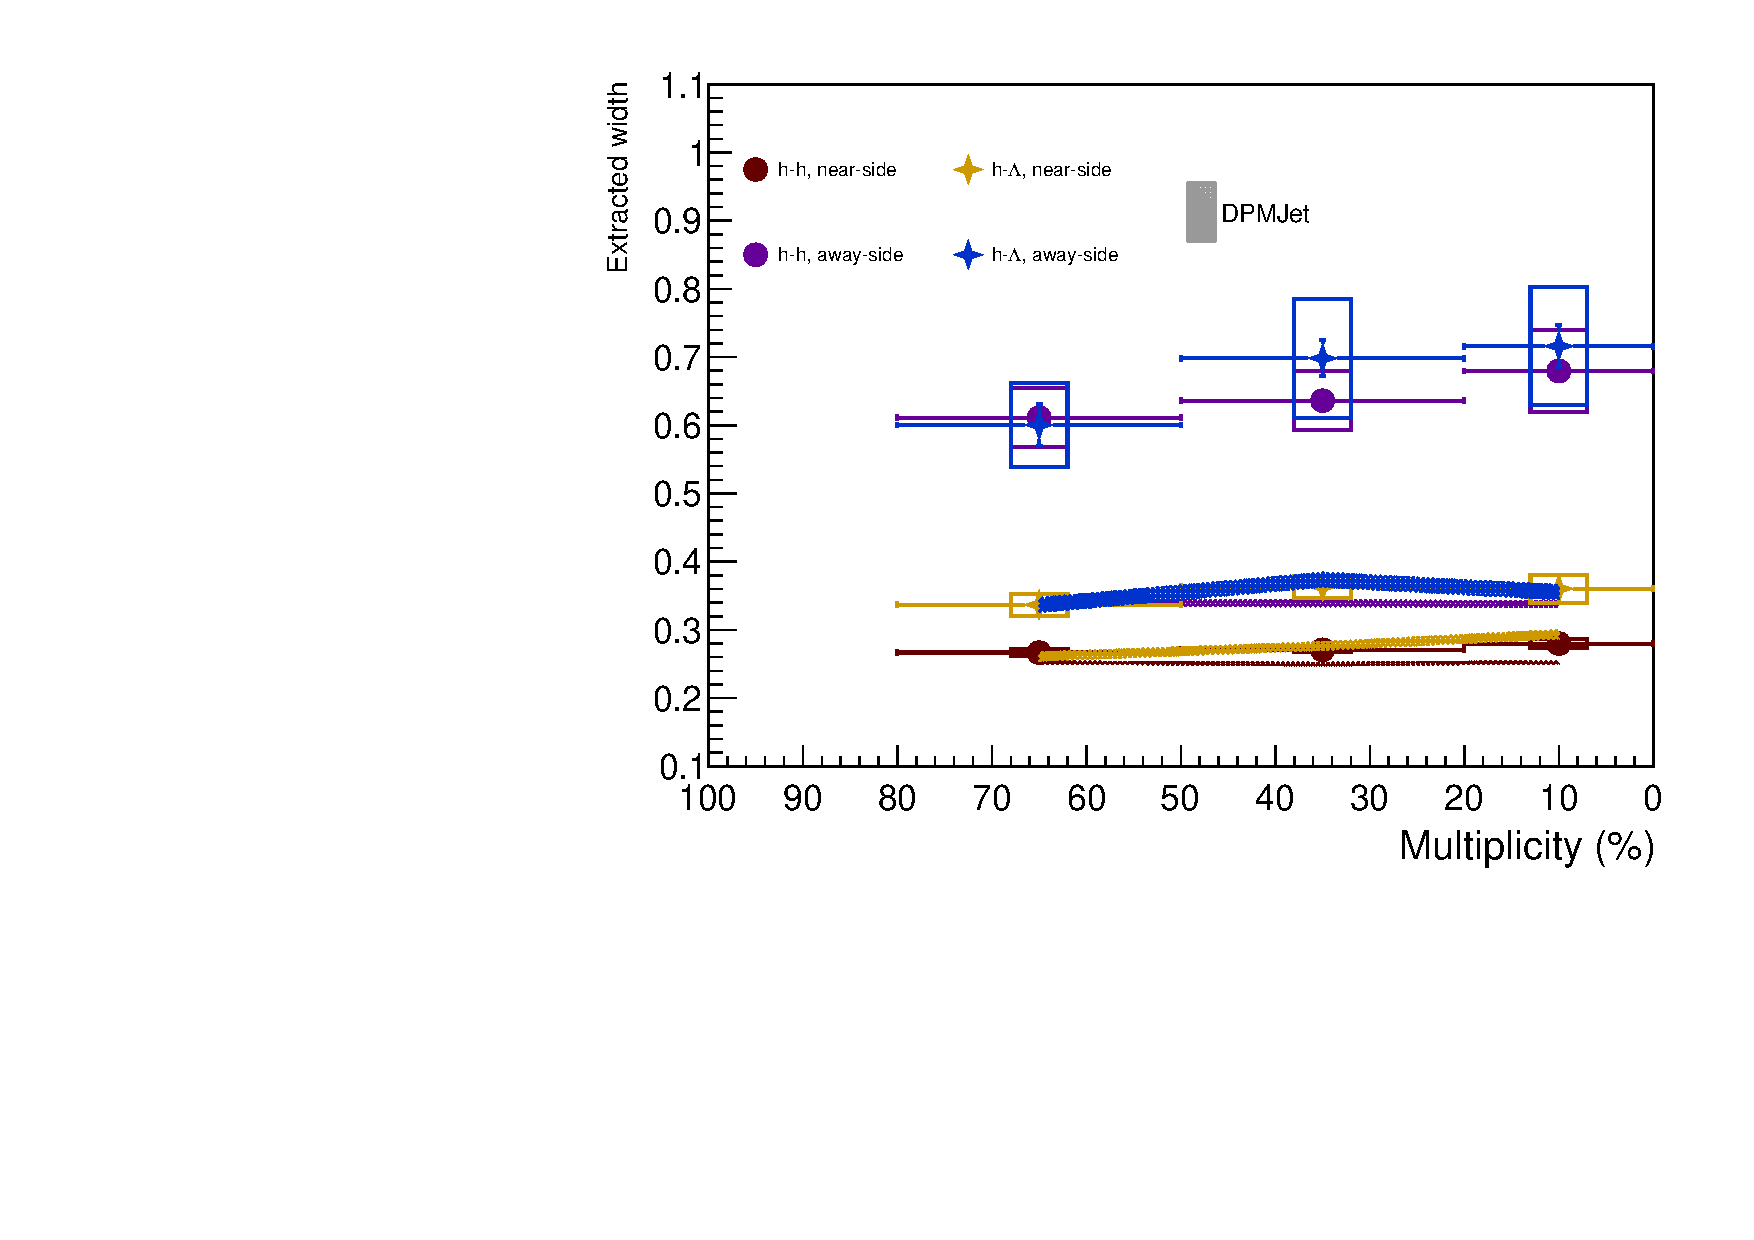
\includegraphics[width=4in]{figures/von_mises_widths_with_dpmjet.pdf}}
\end{subfigure}
\begin{subfigure}{
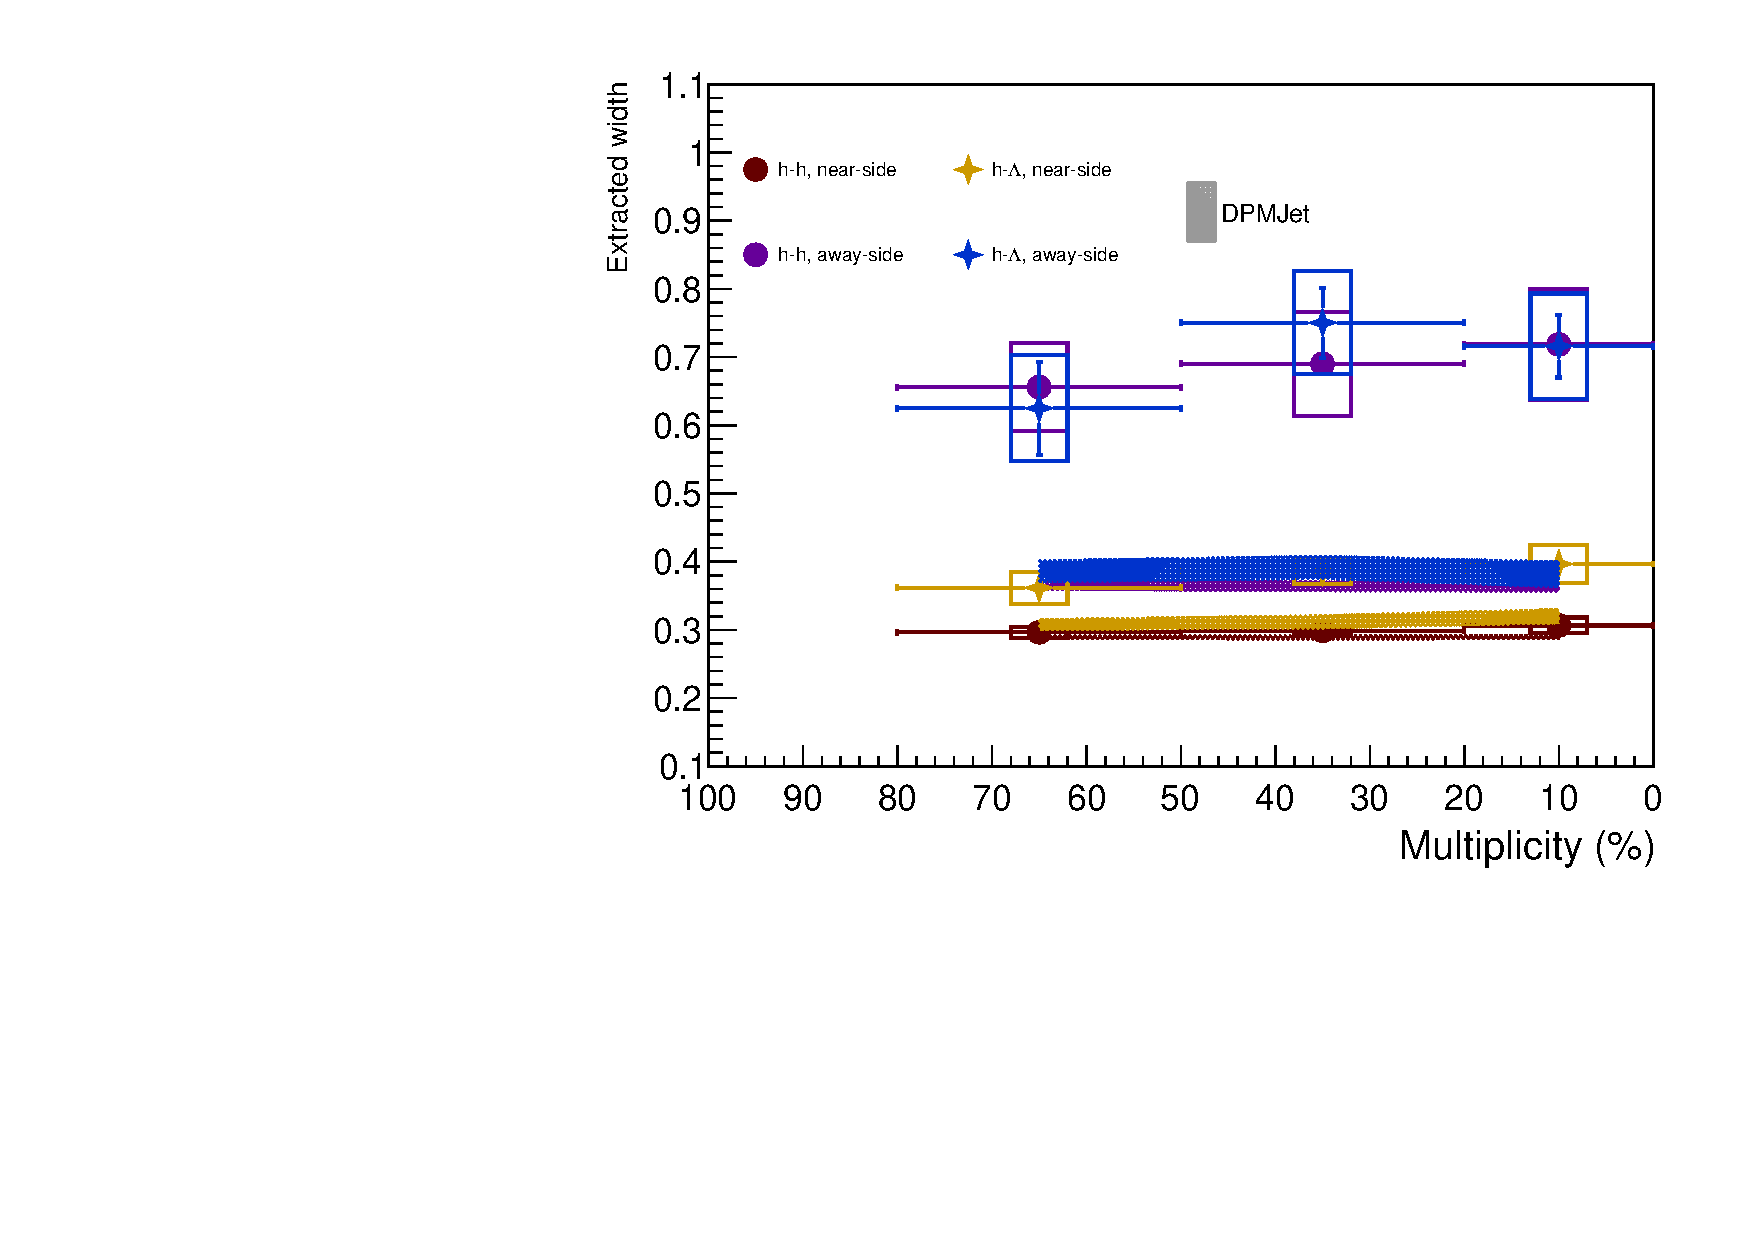
\includegraphics[width=4in]{figures/von_mises_widths_lowpt_with_dpmjet.pdf}}
\end{subfigure}
\begin{subfigure}{
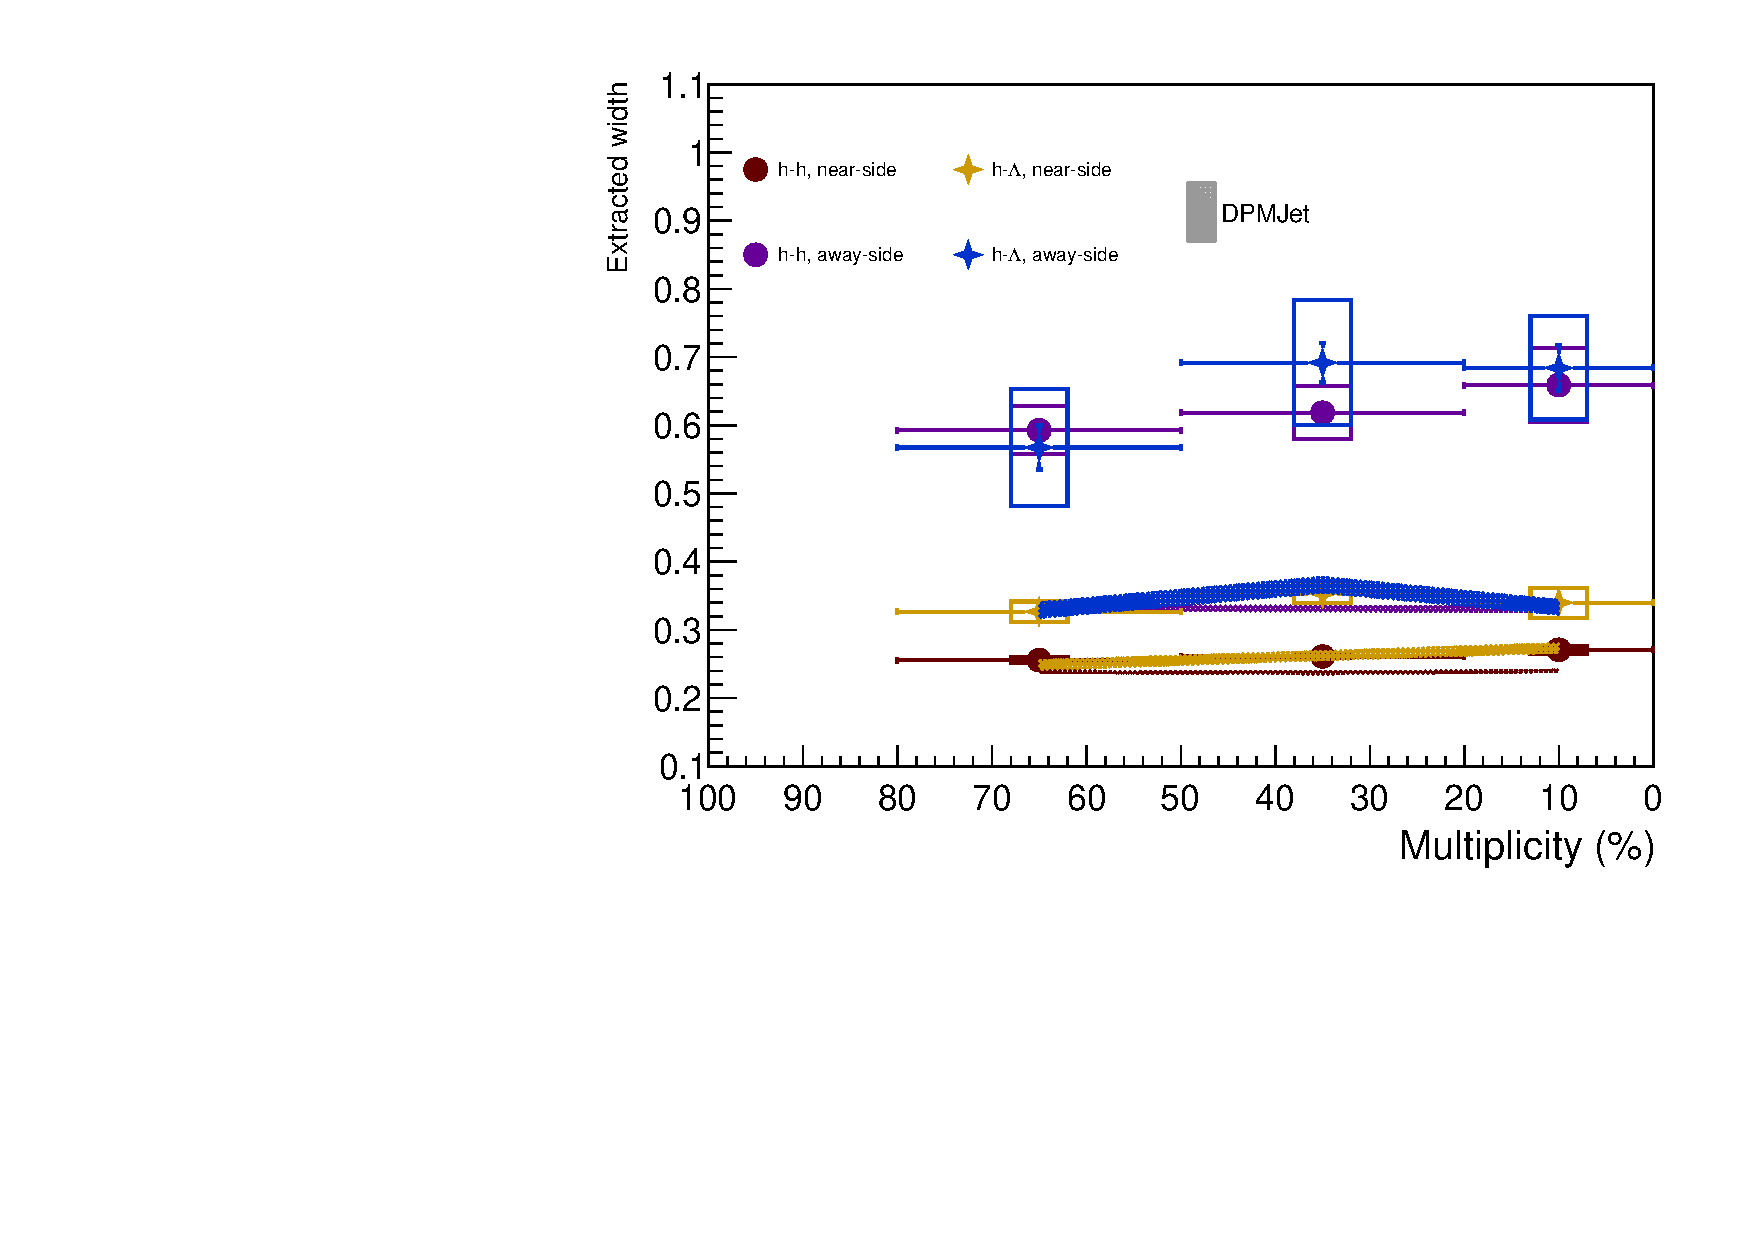
\includegraphics[width=4in]{figures/von_mises_widths_highpt_with_dpmjet.pdf}}
\end{subfigure}
\caption{The widths extracted from the $h-\Lambda$ and $h-h$ $\Delta\varphi$ distributions as a function of multiplicity for each associated $p_{T}$ bin in data and using DPMJet. The top, middle and bottom plots correspond to the 2.0 - 4.0 GeV/c, 1.5 - 2.5 GeV/c and 2.5 - 4.0 GeV/c associated $p_{T}$ bins, respectively.}
\label{width_modelcomp_figure}
\end{figure}